% Capitolul 2: Modele ARMA
% Serii de timp -- Programele de licență Informatică economică și Cibernetică economică, Academia de Studii Economice din București
% GENERAT de latex/build_chapter2.py -- modificați generatorul, nu acest fișier.

\newcommand{\coursename}{Serii de timp}
\def\tsalang{ro}
% Preambul comun TSA -- Serii de timp / Time Series Analysis (Beamer, 16:9)
% Același design ca MFM și SFM (preluat din SFM, 5 octombrie 2026). Înainte de % Preambul comun TSA -- Serii de timp / Time Series Analysis (Beamer, 16:9)
% Același design ca MFM și SFM (preluat din SFM, 5 octombrie 2026). Înainte de % Preambul comun TSA -- Serii de timp / Time Series Analysis (Beamer, 16:9)
% Același design ca MFM și SFM (preluat din SFM, 5 octombrie 2026). Înainte de \input{../../latex/preamble} se definește
%   \newcommand{\coursename}{Time Series Analysis}      (EN)
%   \newcommand{\coursename}{Serii de timp}       (RO)  și  \def\tsalang{ro}
% Fișierele .tex se află în EN/Courses, EN/Seminars, RO/Cursuri, RO/Seminarii (două niveluri sub rădăcină).
% Deck-urile sînt generate de latex/build_chapterN.py / build_seminarN.py (vezi latex/tsa_build.py).

\documentclass[9pt, aspectratio=169, t]{beamer}
\providecommand{\coursename}{Time Series Analysis}

% Ensure content fits on slides
\setbeamersize{text margin left=8mm, text margin right=8mm}
% Smaller institute font (title page)
\setbeamerfont{institute}{size=\footnotesize}

%=============================================================================
% THEME AND STYLE CONFIGURATION
%=============================================================================
\usetheme{default}
% Using default theme for clean header/footer control

% Color Palette (matching Redispatch PDF)
\definecolor{MainBlue}{RGB}{26, 58, 110}
\definecolor{AccentBlue}{RGB}{26, 58, 110}
\definecolor{IDAred}{RGB}{205, 0, 0}
\definecolor{DarkGray}{RGB}{51, 51, 51}
\definecolor{MediumGray}{RGB}{128, 128, 128}
\definecolor{LightGray}{RGB}{248, 248, 248}
\definecolor{VeryLightGray}{RGB}{235, 235, 235}
\definecolor{KeynoteGray}{RGB}{218, 218, 218}
\definecolor{SectionGray}{RGB}{120, 120, 120}
\definecolor{FooterGray}{RGB}{100, 100, 100}
\definecolor{Crimson}{RGB}{220, 53, 69}
\definecolor{Forest}{RGB}{46, 125, 50}
\definecolor{Amber}{RGB}{181, 133, 63}
\definecolor{Orange}{RGB}{230, 126, 34}
\definecolor{Purple}{RGB}{142, 68, 173}

% Gradient background (exact Keynote 315° gradient: white to RGB 218,218,218)
\setbeamertemplate{background}{%
    \begin{tikzpicture}[remember picture, overlay]
        \shade[shading=axis, shading angle=315,
        top color=white, bottom color=KeynoteGray]
        (current page.south west) rectangle (current page.north east);
    \end{tikzpicture}%
}
% Fallback solid color for compatibility
\setbeamercolor{background canvas}{bg=}

\setbeamercolor{palette primary}{bg=MainBlue, fg=white}
\setbeamercolor{palette secondary}{bg=MainBlue!85, fg=white}
\setbeamercolor{palette tertiary}{bg=MainBlue!70, fg=white}
\setbeamercolor{structure}{fg=MainBlue}
\setbeamercolor{title}{fg=IDAred}
\setbeamercolor{frametitle}{fg=IDAred, bg=}
\setbeamercolor{block title}{bg=MainBlue, fg=white}
\setbeamercolor{block body}{bg=VeryLightGray, fg=DarkGray}
\setbeamercolor{block title alerted}{bg=Crimson, fg=white}
\setbeamercolor{block body alerted}{bg=Crimson!8, fg=DarkGray}
\setbeamercolor{block title example}{bg=Forest, fg=white}
\setbeamercolor{block body example}{bg=Forest!8, fg=DarkGray}
\setbeamercolor{item}{fg=MainBlue}

% Footer colors (override Madrid theme blue)
\setbeamercolor{author in head/foot}{fg=FooterGray, bg=}
\setbeamercolor{title in head/foot}{fg=FooterGray, bg=}
\setbeamercolor{date in head/foot}{fg=FooterGray, bg=}
\setbeamercolor{section in head/foot}{fg=FooterGray, bg=}
\setbeamercolor{subsection in head/foot}{fg=FooterGray, bg=}

% Bullet styles (apply everywhere including blocks)
\setbeamertemplate{itemize item}{\color{MainBlue}$\boxdot$}
\setbeamertemplate{itemize subitem}{\color{MainBlue}$\blacktriangleright$}
\setbeamertemplate{itemize subsubitem}{\color{MainBlue}\tiny$\bullet$}
\setbeamertemplate{itemize/enumerate body begin}{\normalsize}
\setbeamertemplate{itemize/enumerate subbody begin}{\normalsize}

% Item spacing - compact style
\setlength{\leftmargini}{10pt}       % Level 1: minimal indent
\setlength{\leftmarginii}{10pt}      % Level 2: minimal additional indent
% Compact list spacing (zero extra space before/after lists in blocks)
\makeatletter
\def\@listi{\leftmargin\leftmargini \topsep 0pt \parsep 0pt \itemsep 0pt}
\def\@listii{\leftmargin\leftmarginii \topsep 0pt \parsep 0pt \itemsep 0pt}
\makeatother

\setbeamertemplate{navigation symbols}{}

%=============================================================================
% CUSTOM HEADLINE
%=============================================================================
\setbeamertemplate{headline}{%
    \vskip10pt%
    \hbox to \paperwidth{%
        \hskip0.5cm%
        {\small\color{FooterGray}\renewcommand{\hyperlink}[2]{##2}\insertsectionhead}%
        \hfill%
        \textcolor{FooterGray}{\small\insertframenumber}%
        \hskip0.5cm%
    }%
    \vskip4pt%
    {\color{FooterGray}\hrule height 0.4pt}%
}

%=============================================================================
% CUSTOM FOOTER
%=============================================================================
\usepackage{fontawesome5}

\setbeamertemplate{footline}{%
    {\color{FooterGray}\hrule height 0.4pt}%
    \vskip4pt%
    \hbox to \paperwidth{%
        \hskip0.5cm%
        \textcolor{FooterGray}{\small\coursename}%
        \hfill%
        \raisebox{-0.1em}{%
            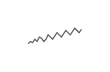
\begin{tikzpicture}[x=0.08em, y=0.08em, line width=0.4pt]
                \draw[FooterGray] (0,3) -- (1,4) -- (2,3.5) -- (3,5) -- (4,4) -- (5,6) -- (6,5.5) -- (7,4) -- (8,5) -- (9,7) -- (10,6) -- (11,5) -- (12,6.5) -- (13,8) -- (14,7) -- (15,6) -- (16,7.5) -- (17,9) -- (18,8) -- (19,7) -- (20,8.5) -- (21,10) -- (22,9) -- (23,8) -- (24,9.5);
            \end{tikzpicture}%
        }%
        \hskip0.5cm%
    }%
    \vskip6pt%
}

%=============================================================================
% PACKAGES
%=============================================================================
\usepackage[utf8]{inputenc}
\DeclareUnicodeCharacter{03B1}{\ensuremath{\alpha}}
\usepackage[T1]{fontenc}
\usepackage{amsmath, amssymb, amsthm}
\usepackage{mathtools}
\usepackage{bm}
\usepackage{tikz}
\usetikzlibrary{arrows.meta, positioning, shapes, calc, decorations.pathreplacing, shadings}
\usepackage{booktabs}
\usepackage{multirow}
\usepackage{array}
\usepackage{graphicx}
\usepackage{animate}
\usepackage{hyperref}
\usepackage{colortbl}
\usepackage{listings}
\lstset{language=Python, basicstyle=\ttfamily\scriptsize, keywordstyle=\color{MainBlue}\bfseries,
  commentstyle=\color{Forest}, stringstyle=\color{Crimson}, breaklines=true,
  frame=none, backgroundcolor=\color{VeryLightGray}, xleftmargin=2mm}
\hypersetup{colorlinks=true, linkcolor=MainBlue, urlcolor=MainBlue}
\graphicspath{{../../logos/}{../../charts/}{../../photos/}}
\usepackage{xcolor}
\hfuzz=2pt  % Suppress tiny overfull warnings (<2pt)
\vfuzz=2pt  % Suppress tiny vertical overfull warnings (<2pt)
% \mathrm in the sans-serif family of the slides (beamer resets \mathrm to the serif family at \begin{document};
% this hook runs after beamer's, so WN, Var, RMSE, ... in formulas match the surrounding text)
% Bold vectors and matrices in the same sans-serif family: \mathbf{A} in sans bold (beamer's own \mathbf came out in
% medium weight), and the bold upright Greek capitals of \boldsymbol / \bm (\bSigma, \bPhi, \boldsymbol{\Theta}) in
% cmss bold: bm.sty fixes its "boldoperators" font when it is loaded (serif cmbx), before beamer switches the
% operators to cmss, so it is reset here.
\AtBeginDocument{%
  \SetMathAlphabet{\mathrm}{normal}{\encodingdefault}{\sfdefault}{\mddefault}{n}%
  \SetMathAlphabet{\mathrm}{bold}{\encodingdefault}{\sfdefault}{bx}{n}%
  \SetMathAlphabet{\mathbf}{normal}{\encodingdefault}{\sfdefault}{bx}{n}%
  \SetMathAlphabet{\mathbf}{bold}{\encodingdefault}{\sfdefault}{bx}{n}%
  \SetSymbolFont{boldoperators}{normal}{OT1}{cmss}{bx}{n}%
  \SetSymbolFont{boldoperators}{bold}{OT1}{cmss}{bx}{n}}

%=============================================================================
% QUANTLET COMMANDS
%   \quantlet{<displayed name>}{<url>}       (generic, compatible with the older TSA decks)
%   \tsaquantlet{Ch_05}{TSA_ch5_garch}       -> https://github.com/danpele/Time-Series-Analysis/tree/main/Quantlets/Ch_05/TSA_ch5_garch
%   \qlurl{<folder>} is defined per chapter by the generator (Quantlets/Ch_NN/<folder>)
%=============================================================================
\newcommand{\tsarepo}{https://github.com/danpele/Time-Series-Analysis}
\newcommand{\tsaqlbase}{https://github.com/danpele/Time-Series-Analysis/tree/main/Quantlets}
\newcommand{\quantlet}[2]{%
    \hfill\href{#2}{%
        \raisebox{-0.15em}{
\includegraphics[height=0.7em]{ql_logo.png}}%
        \textcolor{MainBlue}{\tiny\ #1}%
    }%
}
\newcommand{\tsaquantlet}[2]{\quantlet{\detokenize{#2}}{\tsaqlbase/#1/#2}}

%=============================================================================
% NOTEBOOKS (Google Colab)
%   \colaburl{notebooks/EN/chapter5_seminar_notebook.ipynb} -> the Colab link of a file in the TSA repo
%   \nb: the chapter notebook (each seminar deck redefines it with \renewcommand)
%=============================================================================
\newcommand{\colaburl}[1]{https://colab.research.google.com/github/danpele/Time-Series-Analysis/blob/main/#1}
\newcommand{\nb}{https://colab.research.google.com/github/danpele/Time-Series-Analysis/tree/main/notebooks/EN}
\newcommand{\nbname}{notebooks/EN}

%=============================================================================
% SLIDE HELPERS (used by the generators; the same as in MFM)
%=============================================================================
% local font size for list bodies (the preamble forces \normalsize)
\newcommand{\itemsize}[1]{\setbeamertemplate{itemize/enumerate body begin}{#1}\setbeamertemplate{itemize/enumerate subbody begin}{#1}}
\newcommand{\intitle}[1]{{\hypersetup{urlcolor=white}#1}}   % white links inside coloured title bars
\newcommand{\imgcap}[1]{{\scriptsize #1}\\[0.5mm]}          % caption under a photo
\newcommand{\imgcredit}[2]{{\tiny\color{FooterGray}\href{#1}{#2}}}   % image credit: source URL, author/licence
\newcommand{\aiprompt}[1]{{\ttfamily\color{MainBlue}#1}}     % a prompt to an AI assistant

%=============================================================================
% SEMINARS: student version by default; the instructor wrapper *_solutions.tex sets \solutionstrue
%=============================================================================
\makeatletter\@ifundefined{ifsolutions}{\expandafter\newif\csname ifsolutions\endcsname}{}\makeatother
\newcommand{\solonly}[1]{\ifsolutions #1\fi}
\newcommand{\propsub}{\ifsolutions\else\framesubtitle{\ifdefined\tsalang Rezolvarea se discută la seminar\else Solution discussed in class\fi}\fi}

%=============================================================================
% APPENDIX AND CHAPTER LINKS (latex/appendix_links.py writes the calls; it also re-declares these
% macros before \begin{document}, so the decks compile with or without this preamble block)
%=============================================================================
\providecommand{\tsaapplink}[3]{\hypertarget{#2}{}\hyperlink{#1}{\beamergotobutton{#3}}}
\providecommand{\tsaappback}[2]{\begin{tikzpicture}[remember picture,overlay]\node[anchor=south east] at ([xshift=-3mm,yshift=7mm]current page.south east){\hyperlink{#1}{\beamerreturnbutton{#2}}};\end{tikzpicture}}
\providecommand{\tsachlink}[2]{\href{#1}{#2}}
\providecommand{\tsachlinkt}[2]{\href{#1}{\usebeamercolor[fg]{frametitle}#2}}

%=============================================================================
% QUANTINAR COMMAND: link către un curs Quantinar (subiecte avansate)
%=============================================================================
\newcommand{\quantinar}[2]{%
    \href{#2}{%
        \raisebox{-0.15em}{
\includegraphics[height=0.8em]{qr_logo.png}}%
        \textcolor{MainBlue}{\scriptsize\ #1}%
    }%
}

%=============================================================================
% CUSTOM TITLE PAGE
%=============================================================================
\defbeamertemplate*{title page}{hybrid}[1][]
{
    \vspace{0.2cm}
    % Logos row - top header (with clickable links)
    \begin{center}
        \href{https://www.ase.ro}{
\includegraphics[height=1.0cm]{ase_logo.png}}\hspace{0.3cm}%
        \href{https://theida.net}{
\includegraphics[height=1.0cm]{ida_logo.png}}\hspace{0.3cm}%
        \href{https://blockchain-research-center.com}{
\includegraphics[height=1.0cm]{brc_logo.png}}\hspace{0.3cm}%
        \href{https://www.ai4efin.ase.ro}{
\includegraphics[height=1.0cm]{ai4efin_logo.png}}\hspace{0.3cm}%
        \href{https://ipe.ro/new}{
\includegraphics[height=1.0cm]{acad_logo.png}}\hspace{0.3cm}%
        \href{https://www.digital-finance-msca.com}{
\includegraphics[height=1.0cm]{msca_logo.png}}%
    \end{center}

    \vspace{0.6cm}

    % Main title with Q logos on sides (with clickable links)
    \begin{center}
        \begin{minipage}{0.1\textwidth}
            \centering
            \href{https://quantlet.com}{
\includegraphics[height=1.1cm]{ql_logo.png}}
        \end{minipage}%
        \begin{minipage}{0.78\textwidth}
            \centering
            {\LARGE\bfseries\usebeamercolor[fg]{title}\inserttitle}

            \vspace{0.3cm}

            {\usebeamerfont{subtitle}\usebeamercolor[fg]{title}\insertsubtitle}
        \end{minipage}%
        \begin{minipage}{0.1\textwidth}
            \centering
            \href{https://quantinar.com}{
\includegraphics[height=1.1cm]{qr_logo.png}}
        \end{minipage}
    \end{center}

    \vspace{0.6cm}

    % Authors (left aligned)
    \hspace{0.5cm}{\usebeamerfont{author}\insertauthor}

    \vspace{0.3cm}

    % Institute/Affiliations (left aligned)
    \hspace{0.5cm}\begin{minipage}[t]{0.9\textwidth}
        \raggedright\small\insertinstitute
    \end{minipage}
}

%=============================================================================
% THEOREM ENVIRONMENTS
%=============================================================================
\theoremstyle{definition}
\setbeamertemplate{theorems}[numbered]
\ifdefined\tsalang
\newtheorem{defn}{Definiție}
\newtheorem{thm}{Teoremă}
\newtheorem{prop}{Propoziție}
\newtheorem{rmk}{Observație}
\else
\newtheorem{defn}{Definition}
\newtheorem{thm}{Theorem}
\newtheorem{prop}{Proposition}
\newtheorem{rmk}{Remark}
\fi

%=============================================================================
% CENTRED MINIPAGE (no extra vertical space)
%=============================================================================
\newenvironment{cminipage}[1]{%
    \par\noindent\hfill\begin{minipage}{#1}\ignorespaces
}{%
    \end{minipage}\hfill\null\par
}

%=============================================================================
% CUSTOM COMMANDS
%=============================================================================
\newcommand{\E}{\mathbb{E}}
\newcommand{\Var}{\text{Var}}
\newcommand{\Cov}{\text{Cov}}
\newcommand{\Corr}{\text{Corr}}
\newcommand{\R}{\mathbb{R}}
\newcommand{\N}{\mathbb{N}}
\newcommand{\Z}{\mathbb{Z}}
\newcommand{\B}{\mathbf{B}}
\newcommand{\imark}{\textcolor{MainBlue}{\textbullet}}
\newcommand{\RMSE}{\text{RMSE}}
\newcommand{\MAE}{\text{MAE}}
\newcommand{\MAPE}{\text{MAPE}}

% Boldface vector/matrix commands (VAR, VECM, state space; also used by the older TSA decks)
\newcommand{\bY}{\mathbf{Y}}
\newcommand{\bX}{\mathbf{X}}
\newcommand{\bA}{\mathbf{A}}
\newcommand{\bB}{\mathbf{B}}
\newcommand{\bepsilon}{\boldsymbol{\varepsilon}}
\newcommand{\bSigma}{\boldsymbol{\Sigma}}
\newcommand{\bPhi}{\boldsymbol{\Phi}}
\newcommand{\bGamma}{\boldsymbol{\Gamma}}
\newcommand{\bPi}{\boldsymbol{\Pi}}
\newcommand{\bc}{\mathbf{c}}
\newcommand{\balpha}{\boldsymbol{\alpha}}
\newcommand{\bbeta}{\boldsymbol{\beta}}
\newcommand{\bvarepsilon}{\boldsymbol{\varepsilon}}

% Legacy seminar marks (older TSA seminar decks)
\newcommand{\correct}{\textcolor{Forest}{\checkmark}}
\newcommand{\incorrect}{\textcolor{Crimson}{\texttimes}}
 se definește
%   \newcommand{\coursename}{Time Series Analysis}      (EN)
%   \newcommand{\coursename}{Serii de timp}       (RO)  și  \def\tsalang{ro}
% Fișierele .tex se află în EN/Courses, EN/Seminars, RO/Cursuri, RO/Seminarii (două niveluri sub rădăcină).
% Deck-urile sînt generate de latex/build_chapterN.py / build_seminarN.py (vezi latex/tsa_build.py).

\documentclass[9pt, aspectratio=169, t]{beamer}
\providecommand{\coursename}{Time Series Analysis}

% Ensure content fits on slides
\setbeamersize{text margin left=8mm, text margin right=8mm}
% Smaller institute font (title page)
\setbeamerfont{institute}{size=\footnotesize}

%=============================================================================
% THEME AND STYLE CONFIGURATION
%=============================================================================
\usetheme{default}
% Using default theme for clean header/footer control

% Color Palette (matching Redispatch PDF)
\definecolor{MainBlue}{RGB}{26, 58, 110}
\definecolor{AccentBlue}{RGB}{26, 58, 110}
\definecolor{IDAred}{RGB}{205, 0, 0}
\definecolor{DarkGray}{RGB}{51, 51, 51}
\definecolor{MediumGray}{RGB}{128, 128, 128}
\definecolor{LightGray}{RGB}{248, 248, 248}
\definecolor{VeryLightGray}{RGB}{235, 235, 235}
\definecolor{KeynoteGray}{RGB}{218, 218, 218}
\definecolor{SectionGray}{RGB}{120, 120, 120}
\definecolor{FooterGray}{RGB}{100, 100, 100}
\definecolor{Crimson}{RGB}{220, 53, 69}
\definecolor{Forest}{RGB}{46, 125, 50}
\definecolor{Amber}{RGB}{181, 133, 63}
\definecolor{Orange}{RGB}{230, 126, 34}
\definecolor{Purple}{RGB}{142, 68, 173}

% Gradient background (exact Keynote 315° gradient: white to RGB 218,218,218)
\setbeamertemplate{background}{%
    \begin{tikzpicture}[remember picture, overlay]
        \shade[shading=axis, shading angle=315,
        top color=white, bottom color=KeynoteGray]
        (current page.south west) rectangle (current page.north east);
    \end{tikzpicture}%
}
% Fallback solid color for compatibility
\setbeamercolor{background canvas}{bg=}

\setbeamercolor{palette primary}{bg=MainBlue, fg=white}
\setbeamercolor{palette secondary}{bg=MainBlue!85, fg=white}
\setbeamercolor{palette tertiary}{bg=MainBlue!70, fg=white}
\setbeamercolor{structure}{fg=MainBlue}
\setbeamercolor{title}{fg=IDAred}
\setbeamercolor{frametitle}{fg=IDAred, bg=}
\setbeamercolor{block title}{bg=MainBlue, fg=white}
\setbeamercolor{block body}{bg=VeryLightGray, fg=DarkGray}
\setbeamercolor{block title alerted}{bg=Crimson, fg=white}
\setbeamercolor{block body alerted}{bg=Crimson!8, fg=DarkGray}
\setbeamercolor{block title example}{bg=Forest, fg=white}
\setbeamercolor{block body example}{bg=Forest!8, fg=DarkGray}
\setbeamercolor{item}{fg=MainBlue}

% Footer colors (override Madrid theme blue)
\setbeamercolor{author in head/foot}{fg=FooterGray, bg=}
\setbeamercolor{title in head/foot}{fg=FooterGray, bg=}
\setbeamercolor{date in head/foot}{fg=FooterGray, bg=}
\setbeamercolor{section in head/foot}{fg=FooterGray, bg=}
\setbeamercolor{subsection in head/foot}{fg=FooterGray, bg=}

% Bullet styles (apply everywhere including blocks)
\setbeamertemplate{itemize item}{\color{MainBlue}$\boxdot$}
\setbeamertemplate{itemize subitem}{\color{MainBlue}$\blacktriangleright$}
\setbeamertemplate{itemize subsubitem}{\color{MainBlue}\tiny$\bullet$}
\setbeamertemplate{itemize/enumerate body begin}{\normalsize}
\setbeamertemplate{itemize/enumerate subbody begin}{\normalsize}

% Item spacing - compact style
\setlength{\leftmargini}{10pt}       % Level 1: minimal indent
\setlength{\leftmarginii}{10pt}      % Level 2: minimal additional indent
% Compact list spacing (zero extra space before/after lists in blocks)
\makeatletter
\def\@listi{\leftmargin\leftmargini \topsep 0pt \parsep 0pt \itemsep 0pt}
\def\@listii{\leftmargin\leftmarginii \topsep 0pt \parsep 0pt \itemsep 0pt}
\makeatother

\setbeamertemplate{navigation symbols}{}

%=============================================================================
% CUSTOM HEADLINE
%=============================================================================
\setbeamertemplate{headline}{%
    \vskip10pt%
    \hbox to \paperwidth{%
        \hskip0.5cm%
        {\small\color{FooterGray}\renewcommand{\hyperlink}[2]{##2}\insertsectionhead}%
        \hfill%
        \textcolor{FooterGray}{\small\insertframenumber}%
        \hskip0.5cm%
    }%
    \vskip4pt%
    {\color{FooterGray}\hrule height 0.4pt}%
}

%=============================================================================
% CUSTOM FOOTER
%=============================================================================
\usepackage{fontawesome5}

\setbeamertemplate{footline}{%
    {\color{FooterGray}\hrule height 0.4pt}%
    \vskip4pt%
    \hbox to \paperwidth{%
        \hskip0.5cm%
        \textcolor{FooterGray}{\small\coursename}%
        \hfill%
        \raisebox{-0.1em}{%
            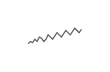
\begin{tikzpicture}[x=0.08em, y=0.08em, line width=0.4pt]
                \draw[FooterGray] (0,3) -- (1,4) -- (2,3.5) -- (3,5) -- (4,4) -- (5,6) -- (6,5.5) -- (7,4) -- (8,5) -- (9,7) -- (10,6) -- (11,5) -- (12,6.5) -- (13,8) -- (14,7) -- (15,6) -- (16,7.5) -- (17,9) -- (18,8) -- (19,7) -- (20,8.5) -- (21,10) -- (22,9) -- (23,8) -- (24,9.5);
            \end{tikzpicture}%
        }%
        \hskip0.5cm%
    }%
    \vskip6pt%
}

%=============================================================================
% PACKAGES
%=============================================================================
\usepackage[utf8]{inputenc}
\DeclareUnicodeCharacter{03B1}{\ensuremath{\alpha}}
\usepackage[T1]{fontenc}
\usepackage{amsmath, amssymb, amsthm}
\usepackage{mathtools}
\usepackage{bm}
\usepackage{tikz}
\usetikzlibrary{arrows.meta, positioning, shapes, calc, decorations.pathreplacing, shadings}
\usepackage{booktabs}
\usepackage{multirow}
\usepackage{array}
\usepackage{graphicx}
\usepackage{animate}
\usepackage{hyperref}
\usepackage{colortbl}
\usepackage{listings}
\lstset{language=Python, basicstyle=\ttfamily\scriptsize, keywordstyle=\color{MainBlue}\bfseries,
  commentstyle=\color{Forest}, stringstyle=\color{Crimson}, breaklines=true,
  frame=none, backgroundcolor=\color{VeryLightGray}, xleftmargin=2mm}
\hypersetup{colorlinks=true, linkcolor=MainBlue, urlcolor=MainBlue}
\graphicspath{{../../logos/}{../../charts/}{../../photos/}}
\usepackage{xcolor}
\hfuzz=2pt  % Suppress tiny overfull warnings (<2pt)
\vfuzz=2pt  % Suppress tiny vertical overfull warnings (<2pt)
% \mathrm in the sans-serif family of the slides (beamer resets \mathrm to the serif family at \begin{document};
% this hook runs after beamer's, so WN, Var, RMSE, ... in formulas match the surrounding text)
% Bold vectors and matrices in the same sans-serif family: \mathbf{A} in sans bold (beamer's own \mathbf came out in
% medium weight), and the bold upright Greek capitals of \boldsymbol / \bm (\bSigma, \bPhi, \boldsymbol{\Theta}) in
% cmss bold: bm.sty fixes its "boldoperators" font when it is loaded (serif cmbx), before beamer switches the
% operators to cmss, so it is reset here.
\AtBeginDocument{%
  \SetMathAlphabet{\mathrm}{normal}{\encodingdefault}{\sfdefault}{\mddefault}{n}%
  \SetMathAlphabet{\mathrm}{bold}{\encodingdefault}{\sfdefault}{bx}{n}%
  \SetMathAlphabet{\mathbf}{normal}{\encodingdefault}{\sfdefault}{bx}{n}%
  \SetMathAlphabet{\mathbf}{bold}{\encodingdefault}{\sfdefault}{bx}{n}%
  \SetSymbolFont{boldoperators}{normal}{OT1}{cmss}{bx}{n}%
  \SetSymbolFont{boldoperators}{bold}{OT1}{cmss}{bx}{n}}

%=============================================================================
% QUANTLET COMMANDS
%   \quantlet{<displayed name>}{<url>}       (generic, compatible with the older TSA decks)
%   \tsaquantlet{Ch_05}{TSA_ch5_garch}       -> https://github.com/danpele/Time-Series-Analysis/tree/main/Quantlets/Ch_05/TSA_ch5_garch
%   \qlurl{<folder>} is defined per chapter by the generator (Quantlets/Ch_NN/<folder>)
%=============================================================================
\newcommand{\tsarepo}{https://github.com/danpele/Time-Series-Analysis}
\newcommand{\tsaqlbase}{https://github.com/danpele/Time-Series-Analysis/tree/main/Quantlets}
\newcommand{\quantlet}[2]{%
    \hfill\href{#2}{%
        \raisebox{-0.15em}{
\includegraphics[height=0.7em]{ql_logo.png}}%
        \textcolor{MainBlue}{\tiny\ #1}%
    }%
}
\newcommand{\tsaquantlet}[2]{\quantlet{\detokenize{#2}}{\tsaqlbase/#1/#2}}

%=============================================================================
% NOTEBOOKS (Google Colab)
%   \colaburl{notebooks/EN/chapter5_seminar_notebook.ipynb} -> the Colab link of a file in the TSA repo
%   \nb: the chapter notebook (each seminar deck redefines it with \renewcommand)
%=============================================================================
\newcommand{\colaburl}[1]{https://colab.research.google.com/github/danpele/Time-Series-Analysis/blob/main/#1}
\newcommand{\nb}{https://colab.research.google.com/github/danpele/Time-Series-Analysis/tree/main/notebooks/EN}
\newcommand{\nbname}{notebooks/EN}

%=============================================================================
% SLIDE HELPERS (used by the generators; the same as in MFM)
%=============================================================================
% local font size for list bodies (the preamble forces \normalsize)
\newcommand{\itemsize}[1]{\setbeamertemplate{itemize/enumerate body begin}{#1}\setbeamertemplate{itemize/enumerate subbody begin}{#1}}
\newcommand{\intitle}[1]{{\hypersetup{urlcolor=white}#1}}   % white links inside coloured title bars
\newcommand{\imgcap}[1]{{\scriptsize #1}\\[0.5mm]}          % caption under a photo
\newcommand{\imgcredit}[2]{{\tiny\color{FooterGray}\href{#1}{#2}}}   % image credit: source URL, author/licence
\newcommand{\aiprompt}[1]{{\ttfamily\color{MainBlue}#1}}     % a prompt to an AI assistant

%=============================================================================
% SEMINARS: student version by default; the instructor wrapper *_solutions.tex sets \solutionstrue
%=============================================================================
\makeatletter\@ifundefined{ifsolutions}{\expandafter\newif\csname ifsolutions\endcsname}{}\makeatother
\newcommand{\solonly}[1]{\ifsolutions #1\fi}
\newcommand{\propsub}{\ifsolutions\else\framesubtitle{\ifdefined\tsalang Rezolvarea se discută la seminar\else Solution discussed in class\fi}\fi}

%=============================================================================
% APPENDIX AND CHAPTER LINKS (latex/appendix_links.py writes the calls; it also re-declares these
% macros before \begin{document}, so the decks compile with or without this preamble block)
%=============================================================================
\providecommand{\tsaapplink}[3]{\hypertarget{#2}{}\hyperlink{#1}{\beamergotobutton{#3}}}
\providecommand{\tsaappback}[2]{\begin{tikzpicture}[remember picture,overlay]\node[anchor=south east] at ([xshift=-3mm,yshift=7mm]current page.south east){\hyperlink{#1}{\beamerreturnbutton{#2}}};\end{tikzpicture}}
\providecommand{\tsachlink}[2]{\href{#1}{#2}}
\providecommand{\tsachlinkt}[2]{\href{#1}{\usebeamercolor[fg]{frametitle}#2}}

%=============================================================================
% QUANTINAR COMMAND: link către un curs Quantinar (subiecte avansate)
%=============================================================================
\newcommand{\quantinar}[2]{%
    \href{#2}{%
        \raisebox{-0.15em}{
\includegraphics[height=0.8em]{qr_logo.png}}%
        \textcolor{MainBlue}{\scriptsize\ #1}%
    }%
}

%=============================================================================
% CUSTOM TITLE PAGE
%=============================================================================
\defbeamertemplate*{title page}{hybrid}[1][]
{
    \vspace{0.2cm}
    % Logos row - top header (with clickable links)
    \begin{center}
        \href{https://www.ase.ro}{
\includegraphics[height=1.0cm]{ase_logo.png}}\hspace{0.3cm}%
        \href{https://theida.net}{
\includegraphics[height=1.0cm]{ida_logo.png}}\hspace{0.3cm}%
        \href{https://blockchain-research-center.com}{
\includegraphics[height=1.0cm]{brc_logo.png}}\hspace{0.3cm}%
        \href{https://www.ai4efin.ase.ro}{
\includegraphics[height=1.0cm]{ai4efin_logo.png}}\hspace{0.3cm}%
        \href{https://ipe.ro/new}{
\includegraphics[height=1.0cm]{acad_logo.png}}\hspace{0.3cm}%
        \href{https://www.digital-finance-msca.com}{
\includegraphics[height=1.0cm]{msca_logo.png}}%
    \end{center}

    \vspace{0.6cm}

    % Main title with Q logos on sides (with clickable links)
    \begin{center}
        \begin{minipage}{0.1\textwidth}
            \centering
            \href{https://quantlet.com}{
\includegraphics[height=1.1cm]{ql_logo.png}}
        \end{minipage}%
        \begin{minipage}{0.78\textwidth}
            \centering
            {\LARGE\bfseries\usebeamercolor[fg]{title}\inserttitle}

            \vspace{0.3cm}

            {\usebeamerfont{subtitle}\usebeamercolor[fg]{title}\insertsubtitle}
        \end{minipage}%
        \begin{minipage}{0.1\textwidth}
            \centering
            \href{https://quantinar.com}{
\includegraphics[height=1.1cm]{qr_logo.png}}
        \end{minipage}
    \end{center}

    \vspace{0.6cm}

    % Authors (left aligned)
    \hspace{0.5cm}{\usebeamerfont{author}\insertauthor}

    \vspace{0.3cm}

    % Institute/Affiliations (left aligned)
    \hspace{0.5cm}\begin{minipage}[t]{0.9\textwidth}
        \raggedright\small\insertinstitute
    \end{minipage}
}

%=============================================================================
% THEOREM ENVIRONMENTS
%=============================================================================
\theoremstyle{definition}
\setbeamertemplate{theorems}[numbered]
\ifdefined\tsalang
\newtheorem{defn}{Definiție}
\newtheorem{thm}{Teoremă}
\newtheorem{prop}{Propoziție}
\newtheorem{rmk}{Observație}
\else
\newtheorem{defn}{Definition}
\newtheorem{thm}{Theorem}
\newtheorem{prop}{Proposition}
\newtheorem{rmk}{Remark}
\fi

%=============================================================================
% CENTRED MINIPAGE (no extra vertical space)
%=============================================================================
\newenvironment{cminipage}[1]{%
    \par\noindent\hfill\begin{minipage}{#1}\ignorespaces
}{%
    \end{minipage}\hfill\null\par
}

%=============================================================================
% CUSTOM COMMANDS
%=============================================================================
\newcommand{\E}{\mathbb{E}}
\newcommand{\Var}{\text{Var}}
\newcommand{\Cov}{\text{Cov}}
\newcommand{\Corr}{\text{Corr}}
\newcommand{\R}{\mathbb{R}}
\newcommand{\N}{\mathbb{N}}
\newcommand{\Z}{\mathbb{Z}}
\newcommand{\B}{\mathbf{B}}
\newcommand{\imark}{\textcolor{MainBlue}{\textbullet}}
\newcommand{\RMSE}{\text{RMSE}}
\newcommand{\MAE}{\text{MAE}}
\newcommand{\MAPE}{\text{MAPE}}

% Boldface vector/matrix commands (VAR, VECM, state space; also used by the older TSA decks)
\newcommand{\bY}{\mathbf{Y}}
\newcommand{\bX}{\mathbf{X}}
\newcommand{\bA}{\mathbf{A}}
\newcommand{\bB}{\mathbf{B}}
\newcommand{\bepsilon}{\boldsymbol{\varepsilon}}
\newcommand{\bSigma}{\boldsymbol{\Sigma}}
\newcommand{\bPhi}{\boldsymbol{\Phi}}
\newcommand{\bGamma}{\boldsymbol{\Gamma}}
\newcommand{\bPi}{\boldsymbol{\Pi}}
\newcommand{\bc}{\mathbf{c}}
\newcommand{\balpha}{\boldsymbol{\alpha}}
\newcommand{\bbeta}{\boldsymbol{\beta}}
\newcommand{\bvarepsilon}{\boldsymbol{\varepsilon}}

% Legacy seminar marks (older TSA seminar decks)
\newcommand{\correct}{\textcolor{Forest}{\checkmark}}
\newcommand{\incorrect}{\textcolor{Crimson}{\texttimes}}
 se definește
%   \newcommand{\coursename}{Time Series Analysis}      (EN)
%   \newcommand{\coursename}{Serii de timp}       (RO)  și  \def\tsalang{ro}
% Fișierele .tex se află în EN/Courses, EN/Seminars, RO/Cursuri, RO/Seminarii (două niveluri sub rădăcină).
% Deck-urile sînt generate de latex/build_chapterN.py / build_seminarN.py (vezi latex/tsa_build.py).

\documentclass[9pt, aspectratio=169, t]{beamer}
\providecommand{\coursename}{Time Series Analysis}

% Ensure content fits on slides
\setbeamersize{text margin left=8mm, text margin right=8mm}
% Smaller institute font (title page)
\setbeamerfont{institute}{size=\footnotesize}

%=============================================================================
% THEME AND STYLE CONFIGURATION
%=============================================================================
\usetheme{default}
% Using default theme for clean header/footer control

% Color Palette (matching Redispatch PDF)
\definecolor{MainBlue}{RGB}{26, 58, 110}
\definecolor{AccentBlue}{RGB}{26, 58, 110}
\definecolor{IDAred}{RGB}{205, 0, 0}
\definecolor{DarkGray}{RGB}{51, 51, 51}
\definecolor{MediumGray}{RGB}{128, 128, 128}
\definecolor{LightGray}{RGB}{248, 248, 248}
\definecolor{VeryLightGray}{RGB}{235, 235, 235}
\definecolor{KeynoteGray}{RGB}{218, 218, 218}
\definecolor{SectionGray}{RGB}{120, 120, 120}
\definecolor{FooterGray}{RGB}{100, 100, 100}
\definecolor{Crimson}{RGB}{220, 53, 69}
\definecolor{Forest}{RGB}{46, 125, 50}
\definecolor{Amber}{RGB}{181, 133, 63}
\definecolor{Orange}{RGB}{230, 126, 34}
\definecolor{Purple}{RGB}{142, 68, 173}

% Gradient background (exact Keynote 315° gradient: white to RGB 218,218,218)
\setbeamertemplate{background}{%
    \begin{tikzpicture}[remember picture, overlay]
        \shade[shading=axis, shading angle=315,
        top color=white, bottom color=KeynoteGray]
        (current page.south west) rectangle (current page.north east);
    \end{tikzpicture}%
}
% Fallback solid color for compatibility
\setbeamercolor{background canvas}{bg=}

\setbeamercolor{palette primary}{bg=MainBlue, fg=white}
\setbeamercolor{palette secondary}{bg=MainBlue!85, fg=white}
\setbeamercolor{palette tertiary}{bg=MainBlue!70, fg=white}
\setbeamercolor{structure}{fg=MainBlue}
\setbeamercolor{title}{fg=IDAred}
\setbeamercolor{frametitle}{fg=IDAred, bg=}
\setbeamercolor{block title}{bg=MainBlue, fg=white}
\setbeamercolor{block body}{bg=VeryLightGray, fg=DarkGray}
\setbeamercolor{block title alerted}{bg=Crimson, fg=white}
\setbeamercolor{block body alerted}{bg=Crimson!8, fg=DarkGray}
\setbeamercolor{block title example}{bg=Forest, fg=white}
\setbeamercolor{block body example}{bg=Forest!8, fg=DarkGray}
\setbeamercolor{item}{fg=MainBlue}

% Footer colors (override Madrid theme blue)
\setbeamercolor{author in head/foot}{fg=FooterGray, bg=}
\setbeamercolor{title in head/foot}{fg=FooterGray, bg=}
\setbeamercolor{date in head/foot}{fg=FooterGray, bg=}
\setbeamercolor{section in head/foot}{fg=FooterGray, bg=}
\setbeamercolor{subsection in head/foot}{fg=FooterGray, bg=}

% Bullet styles (apply everywhere including blocks)
\setbeamertemplate{itemize item}{\color{MainBlue}$\boxdot$}
\setbeamertemplate{itemize subitem}{\color{MainBlue}$\blacktriangleright$}
\setbeamertemplate{itemize subsubitem}{\color{MainBlue}\tiny$\bullet$}
\setbeamertemplate{itemize/enumerate body begin}{\normalsize}
\setbeamertemplate{itemize/enumerate subbody begin}{\normalsize}

% Item spacing - compact style
\setlength{\leftmargini}{10pt}       % Level 1: minimal indent
\setlength{\leftmarginii}{10pt}      % Level 2: minimal additional indent
% Compact list spacing (zero extra space before/after lists in blocks)
\makeatletter
\def\@listi{\leftmargin\leftmargini \topsep 0pt \parsep 0pt \itemsep 0pt}
\def\@listii{\leftmargin\leftmarginii \topsep 0pt \parsep 0pt \itemsep 0pt}
\makeatother

\setbeamertemplate{navigation symbols}{}

%=============================================================================
% CUSTOM HEADLINE
%=============================================================================
\setbeamertemplate{headline}{%
    \vskip10pt%
    \hbox to \paperwidth{%
        \hskip0.5cm%
        {\small\color{FooterGray}\renewcommand{\hyperlink}[2]{##2}\insertsectionhead}%
        \hfill%
        \textcolor{FooterGray}{\small\insertframenumber}%
        \hskip0.5cm%
    }%
    \vskip4pt%
    {\color{FooterGray}\hrule height 0.4pt}%
}

%=============================================================================
% CUSTOM FOOTER
%=============================================================================
\usepackage{fontawesome5}

\setbeamertemplate{footline}{%
    {\color{FooterGray}\hrule height 0.4pt}%
    \vskip4pt%
    \hbox to \paperwidth{%
        \hskip0.5cm%
        \textcolor{FooterGray}{\small\coursename}%
        \hfill%
        \raisebox{-0.1em}{%
            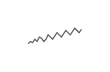
\begin{tikzpicture}[x=0.08em, y=0.08em, line width=0.4pt]
                \draw[FooterGray] (0,3) -- (1,4) -- (2,3.5) -- (3,5) -- (4,4) -- (5,6) -- (6,5.5) -- (7,4) -- (8,5) -- (9,7) -- (10,6) -- (11,5) -- (12,6.5) -- (13,8) -- (14,7) -- (15,6) -- (16,7.5) -- (17,9) -- (18,8) -- (19,7) -- (20,8.5) -- (21,10) -- (22,9) -- (23,8) -- (24,9.5);
            \end{tikzpicture}%
        }%
        \hskip0.5cm%
    }%
    \vskip6pt%
}

%=============================================================================
% PACKAGES
%=============================================================================
\usepackage[utf8]{inputenc}
\DeclareUnicodeCharacter{03B1}{\ensuremath{\alpha}}
\usepackage[T1]{fontenc}
\usepackage{amsmath, amssymb, amsthm}
\usepackage{mathtools}
\usepackage{bm}
\usepackage{tikz}
\usetikzlibrary{arrows.meta, positioning, shapes, calc, decorations.pathreplacing, shadings}
\usepackage{booktabs}
\usepackage{multirow}
\usepackage{array}
\usepackage{graphicx}
\usepackage{animate}
\usepackage{hyperref}
\usepackage{colortbl}
\usepackage{listings}
\lstset{language=Python, basicstyle=\ttfamily\scriptsize, keywordstyle=\color{MainBlue}\bfseries,
  commentstyle=\color{Forest}, stringstyle=\color{Crimson}, breaklines=true,
  frame=none, backgroundcolor=\color{VeryLightGray}, xleftmargin=2mm}
\hypersetup{colorlinks=true, linkcolor=MainBlue, urlcolor=MainBlue}
\graphicspath{{../../logos/}{../../charts/}{../../photos/}}
\usepackage{xcolor}
\hfuzz=2pt  % Suppress tiny overfull warnings (<2pt)
\vfuzz=2pt  % Suppress tiny vertical overfull warnings (<2pt)
% \mathrm in the sans-serif family of the slides (beamer resets \mathrm to the serif family at \begin{document};
% this hook runs after beamer's, so WN, Var, RMSE, ... in formulas match the surrounding text)
% Bold vectors and matrices in the same sans-serif family: \mathbf{A} in sans bold (beamer's own \mathbf came out in
% medium weight), and the bold upright Greek capitals of \boldsymbol / \bm (\bSigma, \bPhi, \boldsymbol{\Theta}) in
% cmss bold: bm.sty fixes its "boldoperators" font when it is loaded (serif cmbx), before beamer switches the
% operators to cmss, so it is reset here.
\AtBeginDocument{%
  \SetMathAlphabet{\mathrm}{normal}{\encodingdefault}{\sfdefault}{\mddefault}{n}%
  \SetMathAlphabet{\mathrm}{bold}{\encodingdefault}{\sfdefault}{bx}{n}%
  \SetMathAlphabet{\mathbf}{normal}{\encodingdefault}{\sfdefault}{bx}{n}%
  \SetMathAlphabet{\mathbf}{bold}{\encodingdefault}{\sfdefault}{bx}{n}%
  \SetSymbolFont{boldoperators}{normal}{OT1}{cmss}{bx}{n}%
  \SetSymbolFont{boldoperators}{bold}{OT1}{cmss}{bx}{n}}

%=============================================================================
% QUANTLET COMMANDS
%   \quantlet{<displayed name>}{<url>}       (generic, compatible with the older TSA decks)
%   \tsaquantlet{Ch_05}{TSA_ch5_garch}       -> https://github.com/danpele/Time-Series-Analysis/tree/main/Quantlets/Ch_05/TSA_ch5_garch
%   \qlurl{<folder>} is defined per chapter by the generator (Quantlets/Ch_NN/<folder>)
%=============================================================================
\newcommand{\tsarepo}{https://github.com/danpele/Time-Series-Analysis}
\newcommand{\tsaqlbase}{https://github.com/danpele/Time-Series-Analysis/tree/main/Quantlets}
\newcommand{\quantlet}[2]{%
    \hfill\href{#2}{%
        \raisebox{-0.15em}{
\includegraphics[height=0.7em]{ql_logo.png}}%
        \textcolor{MainBlue}{\tiny\ #1}%
    }%
}
\newcommand{\tsaquantlet}[2]{\quantlet{\detokenize{#2}}{\tsaqlbase/#1/#2}}

%=============================================================================
% NOTEBOOKS (Google Colab)
%   \colaburl{notebooks/EN/chapter5_seminar_notebook.ipynb} -> the Colab link of a file in the TSA repo
%   \nb: the chapter notebook (each seminar deck redefines it with \renewcommand)
%=============================================================================
\newcommand{\colaburl}[1]{https://colab.research.google.com/github/danpele/Time-Series-Analysis/blob/main/#1}
\newcommand{\nb}{https://colab.research.google.com/github/danpele/Time-Series-Analysis/tree/main/notebooks/EN}
\newcommand{\nbname}{notebooks/EN}

%=============================================================================
% SLIDE HELPERS (used by the generators; the same as in MFM)
%=============================================================================
% local font size for list bodies (the preamble forces \normalsize)
\newcommand{\itemsize}[1]{\setbeamertemplate{itemize/enumerate body begin}{#1}\setbeamertemplate{itemize/enumerate subbody begin}{#1}}
\newcommand{\intitle}[1]{{\hypersetup{urlcolor=white}#1}}   % white links inside coloured title bars
\newcommand{\imgcap}[1]{{\scriptsize #1}\\[0.5mm]}          % caption under a photo
\newcommand{\imgcredit}[2]{{\tiny\color{FooterGray}\href{#1}{#2}}}   % image credit: source URL, author/licence
\newcommand{\aiprompt}[1]{{\ttfamily\color{MainBlue}#1}}     % a prompt to an AI assistant

%=============================================================================
% SEMINARS: student version by default; the instructor wrapper *_solutions.tex sets \solutionstrue
%=============================================================================
\makeatletter\@ifundefined{ifsolutions}{\expandafter\newif\csname ifsolutions\endcsname}{}\makeatother
\newcommand{\solonly}[1]{\ifsolutions #1\fi}
\newcommand{\propsub}{\ifsolutions\else\framesubtitle{\ifdefined\tsalang Rezolvarea se discută la seminar\else Solution discussed in class\fi}\fi}

%=============================================================================
% APPENDIX AND CHAPTER LINKS (latex/appendix_links.py writes the calls; it also re-declares these
% macros before \begin{document}, so the decks compile with or without this preamble block)
%=============================================================================
\providecommand{\tsaapplink}[3]{\hypertarget{#2}{}\hyperlink{#1}{\beamergotobutton{#3}}}
\providecommand{\tsaappback}[2]{\begin{tikzpicture}[remember picture,overlay]\node[anchor=south east] at ([xshift=-3mm,yshift=7mm]current page.south east){\hyperlink{#1}{\beamerreturnbutton{#2}}};\end{tikzpicture}}
\providecommand{\tsachlink}[2]{\href{#1}{#2}}
\providecommand{\tsachlinkt}[2]{\href{#1}{\usebeamercolor[fg]{frametitle}#2}}

%=============================================================================
% QUANTINAR COMMAND: link către un curs Quantinar (subiecte avansate)
%=============================================================================
\newcommand{\quantinar}[2]{%
    \href{#2}{%
        \raisebox{-0.15em}{
\includegraphics[height=0.8em]{qr_logo.png}}%
        \textcolor{MainBlue}{\scriptsize\ #1}%
    }%
}

%=============================================================================
% CUSTOM TITLE PAGE
%=============================================================================
\defbeamertemplate*{title page}{hybrid}[1][]
{
    \vspace{0.2cm}
    % Logos row - top header (with clickable links)
    \begin{center}
        \href{https://www.ase.ro}{
\includegraphics[height=1.0cm]{ase_logo.png}}\hspace{0.3cm}%
        \href{https://theida.net}{
\includegraphics[height=1.0cm]{ida_logo.png}}\hspace{0.3cm}%
        \href{https://blockchain-research-center.com}{
\includegraphics[height=1.0cm]{brc_logo.png}}\hspace{0.3cm}%
        \href{https://www.ai4efin.ase.ro}{
\includegraphics[height=1.0cm]{ai4efin_logo.png}}\hspace{0.3cm}%
        \href{https://ipe.ro/new}{
\includegraphics[height=1.0cm]{acad_logo.png}}\hspace{0.3cm}%
        \href{https://www.digital-finance-msca.com}{
\includegraphics[height=1.0cm]{msca_logo.png}}%
    \end{center}

    \vspace{0.6cm}

    % Main title with Q logos on sides (with clickable links)
    \begin{center}
        \begin{minipage}{0.1\textwidth}
            \centering
            \href{https://quantlet.com}{
\includegraphics[height=1.1cm]{ql_logo.png}}
        \end{minipage}%
        \begin{minipage}{0.78\textwidth}
            \centering
            {\LARGE\bfseries\usebeamercolor[fg]{title}\inserttitle}

            \vspace{0.3cm}

            {\usebeamerfont{subtitle}\usebeamercolor[fg]{title}\insertsubtitle}
        \end{minipage}%
        \begin{minipage}{0.1\textwidth}
            \centering
            \href{https://quantinar.com}{
\includegraphics[height=1.1cm]{qr_logo.png}}
        \end{minipage}
    \end{center}

    \vspace{0.6cm}

    % Authors (left aligned)
    \hspace{0.5cm}{\usebeamerfont{author}\insertauthor}

    \vspace{0.3cm}

    % Institute/Affiliations (left aligned)
    \hspace{0.5cm}\begin{minipage}[t]{0.9\textwidth}
        \raggedright\small\insertinstitute
    \end{minipage}
}

%=============================================================================
% THEOREM ENVIRONMENTS
%=============================================================================
\theoremstyle{definition}
\setbeamertemplate{theorems}[numbered]
\ifdefined\tsalang
\newtheorem{defn}{Definiție}
\newtheorem{thm}{Teoremă}
\newtheorem{prop}{Propoziție}
\newtheorem{rmk}{Observație}
\else
\newtheorem{defn}{Definition}
\newtheorem{thm}{Theorem}
\newtheorem{prop}{Proposition}
\newtheorem{rmk}{Remark}
\fi

%=============================================================================
% CENTRED MINIPAGE (no extra vertical space)
%=============================================================================
\newenvironment{cminipage}[1]{%
    \par\noindent\hfill\begin{minipage}{#1}\ignorespaces
}{%
    \end{minipage}\hfill\null\par
}

%=============================================================================
% CUSTOM COMMANDS
%=============================================================================
\newcommand{\E}{\mathbb{E}}
\newcommand{\Var}{\text{Var}}
\newcommand{\Cov}{\text{Cov}}
\newcommand{\Corr}{\text{Corr}}
\newcommand{\R}{\mathbb{R}}
\newcommand{\N}{\mathbb{N}}
\newcommand{\Z}{\mathbb{Z}}
\newcommand{\B}{\mathbf{B}}
\newcommand{\imark}{\textcolor{MainBlue}{\textbullet}}
\newcommand{\RMSE}{\text{RMSE}}
\newcommand{\MAE}{\text{MAE}}
\newcommand{\MAPE}{\text{MAPE}}

% Boldface vector/matrix commands (VAR, VECM, state space; also used by the older TSA decks)
\newcommand{\bY}{\mathbf{Y}}
\newcommand{\bX}{\mathbf{X}}
\newcommand{\bA}{\mathbf{A}}
\newcommand{\bB}{\mathbf{B}}
\newcommand{\bepsilon}{\boldsymbol{\varepsilon}}
\newcommand{\bSigma}{\boldsymbol{\Sigma}}
\newcommand{\bPhi}{\boldsymbol{\Phi}}
\newcommand{\bGamma}{\boldsymbol{\Gamma}}
\newcommand{\bPi}{\boldsymbol{\Pi}}
\newcommand{\bc}{\mathbf{c}}
\newcommand{\balpha}{\boldsymbol{\alpha}}
\newcommand{\bbeta}{\boldsymbol{\beta}}
\newcommand{\bvarepsilon}{\boldsymbol{\varepsilon}}

% Legacy seminar marks (older TSA seminar decks)
\newcommand{\correct}{\textcolor{Forest}{\checkmark}}
\newcommand{\incorrect}{\textcolor{Crimson}{\texttimes}}


\newcommand{\qlurl}[1]{https://github.com/danpele/Time-Series-Analysis/tree/main/Quantlets/Ch_02/#1}

% Clickable citations (DOIs verified via Crossref)
\newcommand{\refHP}{\href{https://doi.org/10.1007/978-3-031-13584-2}{Huang și Petukhina (2022)}}
\newcommand{\refFPP}{\href{https://otexts.com/fpp3/arima.html}{Hyndman și Athanasopoulos (2021)}}
\newcommand{\refBD}{\href{https://doi.org/10.1007/978-3-319-29854-2}{Brockwell și Davis (2016)}}
\newcommand{\refBDtm}{\href{https://doi.org/10.1007/978-1-4419-0320-4}{Brockwell și Davis (1991)}}
\newcommand{\refHamilton}{\href{https://doi.org/10.2307/j.ctv14jx6sm}{Hamilton (1994)}}
\newcommand{\refBJ}{\href{https://doi.org/10.1002/9781118619193}{Box, Jenkins și Reinsel (2008)}}
\newcommand{\refBP}{\href{https://doi.org/10.1080/01621459.1970.10481180}{Box și Pierce (1970)}}
\newcommand{\refLB}{\href{https://doi.org/10.1093/biomet/65.2.297}{Ljung și Box (1978)}}
\newcommand{\refYule}{\href{https://doi.org/10.1098/rsta.1927.0007}{Yule (1927)}}
\newcommand{\refWalker}{\href{https://doi.org/10.1098/rspa.1931.0069}{Walker (1931)}}
\newcommand{\refSlutzky}{\href{https://doi.org/10.2307/1907241}{Slutzky (1937)}}
\newcommand{\refWold}{\href{https://archive.org/details/in.ernet.dli.2015.262214}{Wold (1938)}}
\newcommand{\refDurbin}{\href{https://doi.org/10.2307/1401322}{Durbin (1960)}}
\newcommand{\refAkaike}{\href{https://doi.org/10.1109/TAC.1974.1100705}{Akaike (1974)}}
\newcommand{\refSchwarz}{\href{https://doi.org/10.1214/aos/1176344136}{Schwarz (1978)}}
\newcommand{\refHT}{\href{https://doi.org/10.1093/biomet/76.2.297}{Hurvich și Tsai (1989)}}
\newcommand{\refJB}{\href{https://doi.org/10.2307/1403192}{Jarque și Bera (1987)}}
\newcommand{\refHK}{\href{https://doi.org/10.18637/jss.v027.i03}{Hyndman și Khandakar (2008)}}
\newcommand{\refMH}{\href{https://doi.org/10.1016/S0169-2070(00)00057-1}{Makridakis și Hibon (2000)}}

\title[Serii de timp]{Serii de timp}
\subtitle{Capitolul 2: Modele ARMA}
\author[D.T. Pele]{Daniel Traian PELE}
\institute{Academia de Studii Economice din București\\
IDA Institute Digital Assets\\
Blockchain Research Center\\
AI4EFin Artificial Intelligence for Energy Finance\\
Academia Română, Institutul de Prognoză Economică\\
MSCA Digital Finance}
\date{}

%=============================================================================
\providecommand{\tsaapplink}[3]{\hypertarget{#2}{}\hyperlink{#1}{\beamergotobutton{#3}}}  % APPLINKS-MACROS
\providecommand{\tsaappback}[2]{\begin{tikzpicture}[remember picture,overlay]\node[anchor=south east] at ([xshift=-3mm,yshift=7mm]current page.south east){\hyperlink{#1}{\beamerreturnbutton{#2}}};\end{tikzpicture}}  % APPLINKS-MACROS
\providecommand{\tsachlink}[2]{\href{#1}{#2}}  % APPLINKS-MACROS
\providecommand{\tsachlinkt}[2]{\href{#1}{\usebeamercolor[fg]{frametitle}#2}}  % APPLINKS-MACROS
\begin{document}
%=============================================================================

{
\setbeamertemplate{headline}{}
\setbeamertemplate{footline}{}
\begin{frame}[noframenumbering]
    \titlepage
\end{frame}
}
% BEGIN-ACRONYMS (generat de latex/acronyms.py; nu editati manual)
\begin{frame}{Acronime folosite în acest material}
\setbeamertemplate{itemize/enumerate body begin}{\tiny}
\begin{columns}[T]
\begin{column}{0.49\textwidth}
\begin{itemize}\setlength{\itemsep}{0pt}
    \item \textbf{ACF}: Autocorrelation Function (funcția de autocorelație)
    \item \textbf{AI}: Artificial Intelligence (inteligență artificială)
    \item \textbf{AIC}: Akaike Information Criterion (criteriul informațional Akaike)
    \item \textbf{AR}: AutoRegressive (model) — model autoregresiv
    \item \textbf{ARIMA}: AutoRegressive Integrated Moving Average (model) — model autoregresiv integrat cu medie mobilă
    \item \textbf{ARMA}: AutoRegressive Moving Average (model) — model autoregresiv cu medie mobilă
    \item \textbf{BET}: Bucharest Exchange Trading (index) — indicele de referință al Bursei de Valori București
    \item \textbf{BIC}: Bayesian Information Criterion (criteriul informațional bayesian (Schwarz))
    \item \textbf{BNR}: Banca Națională a României
    \item \textbf{GARCH}: Generalised AutoRegressive Conditional Heteroskedasticity (heteroscedasticitate condiționată autoregresivă generalizată)
    \item \textbf{GDP}: Gross Domestic Product (produsul intern brut)
    \item \textbf{IAPC}: Indicele armonizat al prețurilor de consum
    \item \textbf{INS}: Institutul Național de Statistică
\end{itemize}
\end{column}
\begin{column}{0.49\textwidth}
\begin{itemize}\setlength{\itemsep}{0pt}
    \item \textbf{LB}: Ljung–Box (test) — testul de autocorelație Ljung–Box
    \item \textbf{MA}: Moving Average (medie mobilă)
    \item \textbf{MLE}: Maximum Likelihood Estimation (estimarea prin metoda verosimilității maxime)
    \item \textbf{MSE}: Mean Squared Error (eroarea pătratică medie)
    \item \textbf{OLS}: Ordinary Least Squares (metoda celor mai mici pătrate)
    \item \textbf{PACF}: Partial AutoCorrelation Function (funcția de autocorelație parțială)
    \item \textbf{PIB}: Produsul intern brut
    \item \textbf{QQ}: Quantile–Quantile (plot) — graficul cuantilă–cuantilă
    \item \textbf{UE}: Uniunea Europeană
    \item \textbf{VAR}: Vector AutoRegression (model vector autoregresiv)
\end{itemize}
\end{column}
\end{columns}
\end{frame}
% END-ACRONYMS

\begin{frame}{Întrebarea de azi și traseul}
\itemsize{\small}
\begin{itemize}
    \item \textbf{Întrebarea}: o serie staționară este corelată cu propriul trecut; ce model mic surprinde această memorie și o transformă în prognoze cu o incertitudine corect măsurată?
    \begin{itemize}
        \item răspunsul lui Box și Jenkins: modelele \textbf{ARMA($p,q$)}, cîțiva parametri în locul infinității de ponderi Wold
    \end{itemize}
    \item \textbf{Traseul} capitolului
    \begin{itemize}
        \item AR($p$) și MA($q$): staționaritate, invertibilitate, rădăcini caracteristice, ACF și PACF
        \item ARMA($p,q$): forma cauzală MA($\infty$), răspunsurile la impuls, identificarea
        \item estimarea (Yule--Walker, cele mai mici pătrate condiționate, verosimilitate maximă), AIC și BIC, diagnosticarea reziduurilor
        \item prognoza și metoda Box--Jenkins pe PIB-ul și inflația României, BET, EUR/RON și petele solare
    \end{itemize}
    \item Seminarul 2 are loc înaintea acestui curs: dă formulele; aici le deducem și le aplicăm pe date
\end{itemize}
\end{frame}

\begin{frame}{Rezultatele învățării}
\itemsize{\small}
\begin{itemize}
    \item Verificați staționaritatea unui AR($p$) și invertibilitatea unui MA($q$) din rădăcinile polinoamelor lor
    \item Deduceți media, autocovarianțele și ponderile $\psi$ pentru AR(1), AR(2), MA($q$) și ARMA(1,1)
    \item Propuneți ordine candidate din ACF și PACF și alegeți între ele cu AIC și BIC
    \item Estimați modele ARMA prin Yule--Walker, cele mai mici pătrate condiționate și verosimilitate maximă și interpretați rezultatele
    \item Testați reziduurile: Ljung--Box cu $m - p - q$ grade de libertate, Jarque--Bera
    \item Calculați prognozele ARMA și intervalele lor și explicați revenirea la medie
\end{itemize}
\end{frame}

\begin{frame}{Bibliografie și instrumente}
\itemsize{\small}
\begin{itemize}
    \item Manual: \refHP, cap.~3--4 (modele staționare, ARMA)
    \begin{itemize}
        \item manual însoțitor, gratuit online: \refFPP, cap.~9 (modele ARIMA)
    \end{itemize}
    \item Teorie: \refBD, cap.~3 (ARMA) și cap.~5 (estimare); \refHamilton, cap.~3--5; lucrarea clasică: \refBJ
    \item Quantlet-urile Python ale capitolului: \href{https://github.com/danpele/Time-Series-Analysis/tree/main/Quantlets/Ch_02}{Quantlets/Ch\_02}
    \begin{itemize}
        \item estimarea ARMA cu \texttt{statsmodels} (\texttt{ARIMA}, \texttt{ArmaProcess}, \texttt{acorr\_ljungbox})
    \end{itemize}
    \item Notebook-ul cursului: \href{\colaburl{notebooks/EN/chapter2_lecture_notebook.ipynb}}{deschideți în Google Colab}
    \item Curs video: \quantinar{Applied Time Series Analysis with Python}{https://quantinar.com/course/137/applied-time-series-analysis-with-python}
\end{itemize}
\end{frame}


%=============================================================================
\section{De la Capitolul 1 la modelele ARMA}
%=============================================================================

\begin{frame}{Instrumente din \tsachlinkt{https://danpele.github.io/Time-Series-Analysis/RO/Cursuri/capitol1_procese_stochastice_stationaritate.pdf}{Capitolul 1}}
\itemsize{\small}
\begin{itemize}
    \item \textbf{Staționaritatea slabă}: media constantă $\mu$ și autocovarianța $\gamma(h) = \mathrm{Cov}(X_t, X_{t+h})$, care depinde doar de decalajul $h$
    \begin{itemize}
        \item ACF $\rho(h) = \gamma(h)/\gamma(0)$; PACF $\phi_{hh}$ = corelația dintre $X_t$ și $X_{t+h}$ după eliminarea efectului lui $X_{t+1}, \dots, X_{t+h-1}$
    \end{itemize}
    \item \textbf{Zgomotul alb} $\varepsilon_t \sim \mathrm{WN}(0, \sigma^2)$: media 0, varianța $\sigma^2$, fără autocorelație
    \begin{itemize}
        \item \textbf{operatorul lag}: $LX_t = X_{t-1}$, $L^kX_t = X_{t-k}$; polinoamele în $L$ acționează asupra seriilor
    \end{itemize}
    \item \textbf{Descompunerea Wold} (\refWold): orice proces staționar pur nedeterminist este $X_t = \mu + \sum_{j \ge 0}\psi_j\varepsilon_{t-j}$, $\psi_0 = 1$, $\sum_j\psi_j^2 < \infty$
    \begin{itemize}
        \item detalii și grafice: \tsachlink{https://danpele.github.io/Time-Series-Analysis/RO/Cursuri/capitol1_procese_stochastice_stationaritate.pdf}{Capitolul 1}, secțiunile despre operatorul lag, descompunerea Wold și ACF și PACF de selecție
    \end{itemize}
\end{itemize}
\end{frame}

\begin{frame}{Problema: o infinitate de ponderi}
\itemsize{\small}
\begin{itemize}
    \item Teorema Wold spune \textbf{cum arată} un proces staționar, nu \textbf{cum îl estimăm}
    \begin{itemize}
        \item $\psi_1, \psi_2, \dots$: o infinitate de necunoscute și doar $T$ observații
    \end{itemize}
    \item \textbf{Ideea}: scriem $\psi(L) = \sum_j\psi_jL^j$ ca \textbf{raport a două polinoame scurte}
    \begin{itemize}
        \item $\psi(L) = \theta(L)/\phi(L)$, cu $\phi(L) = 1 - \phi_1L - \dots - \phi_pL^p$, $\theta(L) = 1 + \theta_1L + \dots + \theta_qL^q$
        \item atunci $\phi(L)(X_t - \mu) = \theta(L)\varepsilon_t$: modelul \textbf{ARMA($p,q$)}, cu $p + q + 2$ parametri ($\phi$, $\theta$, $\mu$, $\sigma^2$)
    \end{itemize}
    \item O funcție rațională aproximează bine aproape orice $\psi(L)$ netedă, cu $p$ și $q$ mici
    \begin{itemize}
        \item principiul \textbf{parcimoniei}: cel mai mic model care lasă reziduuri de tip zgomot alb
    \end{itemize}
\end{itemize}
\end{frame}

\begin{frame}{Trei piese de bază}
\itemsize{\small}
\begin{itemize}
    \item \textbf{AR($p$)}, autoregresiv: valoarea de azi depinde de ultimele $p$ valori ale seriei
    \begin{itemize}
        \item $X_t = c + \phi_1X_{t-1} + \dots + \phi_pX_{t-p} + \varepsilon_t$; originea: \refYule, petele solare
    \end{itemize}
    \item \textbf{MA($q$)}, medie mobilă: valoarea de azi depinde de ultimele $q$ șocuri
    \begin{itemize}
        \item $X_t = \mu + \varepsilon_t + \theta_1\varepsilon_{t-1} + \dots + \theta_q\varepsilon_{t-q}$; originea: \refSlutzky, sume de cauze aleatoare
    \end{itemize}
    \item \textbf{ARMA($p,q$)}: ambele părți; transformat într-o metodă completă de \refBJ{} (prima ediție în 1970)
    \begin{itemize}
        \item $c$ este \textbf{termenul liber}; media este $\mu = c/(1 - \phi_1 - \dots - \phi_p)$, nu $c$
    \end{itemize}
    \item Peste tot: $\varepsilon_t \sim \mathrm{WN}(0, \sigma^2)$, iar pentru verosimilitate și intervale $\varepsilon_t$ i.i.d. $N(0, \sigma^2)$ (independente și identic distribuite)
\end{itemize}
\end{frame}


%=============================================================================
\section{Modele autoregresive}
%=============================================================================

\begin{frame}{Modelul AR(1)}
\itemsize{\small}
\begin{itemize}
    \item $X_t = c + \phi X_{t-1} + \varepsilon_t$, sau $(1 - \phi L)X_t = c + \varepsilon_t$
    \begin{itemize}
        \item $\phi$: partea din abaterea de azi față de medie care se păstrează și mîine
    \end{itemize}
    \item \textbf{Substituind înapoi} de $k$ ori:
    \begin{itemize}
        \item $X_t = c(1 + \phi + \dots + \phi^{k-1}) + \phi^kX_{t-k} + \sum_{j=0}^{k-1}\phi^j\varepsilon_{t-j}$
        \item dacă $|\phi| < 1$: $\phi^k \to 0$ și $X_t = \dfrac{c}{1 - \phi} + \sum_{j=0}^{\infty}\phi^j\varepsilon_{t-j}$
    \end{itemize}
    \item Aceasta este forma Wold cu $\psi_j = \phi^j$: reprezentarea \textbf{cauzală} (MA($\infty$))
    \begin{itemize}
        \item cauzală = $X_t$ depinde doar de șocurile prezente și trecute
        \item $\phi = 1$: mers aleator (\tsachlink{https://danpele.github.io/Time-Series-Analysis/RO/Cursuri/capitol1_procese_stochastice_stationaritate.pdf}{Capitolul 1}), fără soluție staționară; $|\phi| > 1$: proces exploziv sau o soluție care depinde de șocuri viitoare, exclusă
    \end{itemize}
\end{itemize}
\end{frame}

\begin{frame}{Momentele unui AR(1) staționar}
\itemsize{\small}
\begin{itemize}
    \item \textbf{Media}: aplicăm media, $\mu = c + \phi\mu$, deci $\mu = c/(1 - \phi)$
    \begin{itemize}
        \item aici folosim staționaritatea: $E[X_t] = E[X_{t-1}]$
    \end{itemize}
    \item \textbf{Varianța}: $\gamma(0) = \phi^2\gamma(0) + \sigma^2$, deoarece $\varepsilon_t$ este necorelat cu $X_{t-1}$
    \begin{itemize}
        \item $\gamma(0) = \sigma^2/(1 - \phi^2)$: crește nelimitat cînd $|\phi| \to 1$
    \end{itemize}
    \item \textbf{Autocovarianțele}: înmulțim $X_t - \mu = \phi(X_{t-1} - \mu) + \varepsilon_t$ cu $X_{t-h} - \mu$, $h \ge 1$, și aplicăm media
    \begin{itemize}
        \item $\gamma(h) = \phi\gamma(h - 1)$, deci $\gamma(h) = \phi^h\gamma(0)$ și $\rho(h) = \phi^h$
        \item descreștere geometrică; semne alternante dacă $\phi < 0$
    \end{itemize}
    \item \textbf{Timpul de înjumătățire} al unui șoc: $h$ pentru care $\phi^h = 1/2$, adică $h = \ln 0{,}5/\ln\phi$
\end{itemize}
\end{frame}

\begin{frame}{Exemplu rezolvat: un AR(1)}
\itemsize{\small}
\begin{itemize}
    \item $X_t = 2 + 0{,}8X_{t-1} + \varepsilon_t$, $\sigma^2 = 1$
    \item Este staționar? $|\phi| = 0{,}8 < 1$: da
    \begin{itemize}
        \item media $\mu = 2/(1 - 0{,}8) = 10$; termenul liber este 2, media este 10
    \end{itemize}
    \item Varianța și ACF
    \begin{itemize}
        \item $\gamma(0) = 1/(1 - 0{,}64) = 2{,}78$
        \item $\rho(3) = 0{,}8^3 = 0{,}512$
    \end{itemize}
    \item Timpul de înjumătățire $= \ln 0{,}5/\ln 0{,}8 = 3{,}11$ perioade
    \begin{itemize}
        \item după aproximativ 3 perioade, jumătate din șoc a dispărut
    \end{itemize}
    \item Ponderile $\psi$: $1; 0{,}8; 0{,}64; 0{,}512; \dots$: un șoc de 1 azi îl mută pe $X_{t+2}$ cu $0{,}64$
\end{itemize}
\end{frame}

\begin{frame}{AR(1) pentru trei valori ale lui $\phi$}
\itemsize{\footnotesize}
\begin{center}
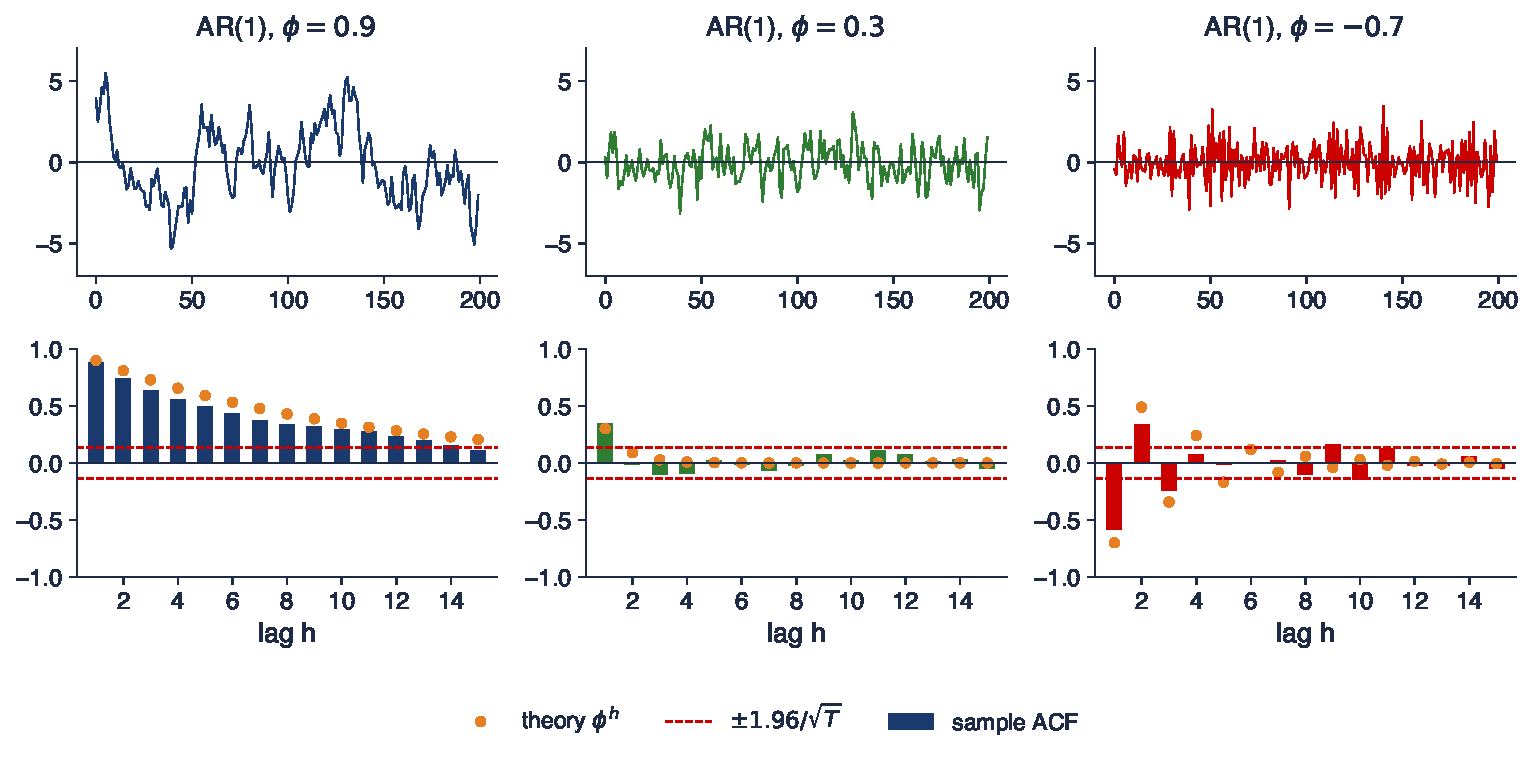
\includegraphics[width=0.97\textwidth,height=0.72\textheight,keepaspectratio]{tsa_ch2_ar1.pdf}
\end{center}
\vspace{-0.25cm}
\begin{itemize}
    \item Aceleași 200 de șocuri, $\phi = 0{,}9$; $0{,}3$; $-0{,}7$; jos: ACF de selecție (bare) și $\rho(h) = \phi^h$ (puncte)
\end{itemize}
\quantlet{TSA\_ch2\_ar\_models}{\qlurl{TSA_ch2_ar_models}}
\end{frame}

\begin{frame}{Interpretarea traiectoriilor AR(1)}
\itemsize{\small}
\begin{itemize}
    \item $\phi = 0{,}9$: abateri lungi de la 0; $\hat\rho(1) = 0{,}88$ de selecție, varianța 4{,}98 (teoretic 5{,}26)
    \begin{itemize}
        \item persistența puternică seamănă cu un trend pe ferestre scurte
    \end{itemize}
    \item $\phi = 0{,}3$: aproape de zgomot alb; doar $\hat\rho(1) = 0{,}35$ iese clar din bandă
    \begin{itemize}
        \item varianța 1{,}18 (teoretic 1{,}10)
    \end{itemize}
    \item $\phi = -0{,}7$: zigzag; $\hat\rho(1) = -0{,}58$, $\hat\rho(2) = 0{,}34$, semne alternante
    \begin{itemize}
        \item în economie: depășire și corecție sau o eroare de măsurare corectată în perioada următoare
    \end{itemize}
    \item Cu $T = 200$, ACF de selecție este sub cea teoretică la decalaje mari: o deplasare de eșantion mic, care afectează și estimatorii (secțiunea 5)
\end{itemize}
\end{frame}

\begin{frame}{Modelul AR($p$) și polinomul lui caracteristic}
\itemsize{\small}
\begin{itemize}
    \item $\phi(L)X_t = c + \varepsilon_t$, cu $\phi(z) = 1 - \phi_1z - \dots - \phi_pz^p$, un polinom într-un număr complex $z$
    \begin{itemize}
        \item factorizăm: $\phi(z) = (1 - \lambda_1z)\cdots(1 - \lambda_pz)$, unde $z_i = 1/\lambda_i$ sînt rădăcinile
    \end{itemize}
    \item \textbf{Condiția de staționaritate (cauzalitate)}: toate rădăcinile lui $\phi(z) = 0$ sînt \textbf{în afara cercului unitate}, $|z_i| > 1$
    \begin{itemize}
        \item echivalent: toate \textbf{rădăcinile inverse} $\lambda_i$ sînt în interior, $|\lambda_i| < 1$ (forma afișată de programe)
        \item motivul: $1/(1 - \lambda L) = \sum_j\lambda^jL^j$ converge doar dacă $|\lambda| < 1$; fiecare factor este un AR(1)
    \end{itemize}
    \item O rădăcină pe cerc ($|z| = 1$, de exemplu $z = 1$) este o \textbf{rădăcină unitară}: nestaționaritate, subiectul \tsachlink{https://danpele.github.io/Time-Series-Analysis/RO/Cursuri/capitol3_radacini_unitare_modele_arima.pdf}{Capitolului 3}
    \begin{itemize}
        \item verificare rapidă, necesară: $\phi_1 + \dots + \phi_p < 1$ (adică $\phi(1) > 0$)
    \end{itemize}
\end{itemize}
\end{frame}

\begin{frame}{AR(2): triunghiul de staționaritate}
\itemsize{\small}
\begin{itemize}
    \item $X_t = \phi_1X_{t-1} + \phi_2X_{t-2} + \varepsilon_t$ este staționar dacă și numai dacă
    \begin{itemize}
        \item $\phi_1 + \phi_2 < 1$, \quad $\phi_2 - \phi_1 < 1$, \quad $|\phi_2| < 1$
    \end{itemize}
    \item Rădăcinile sînt complexe cînd $\phi_1^2 + 4\phi_2 < 0$
    \begin{itemize}
        \item atunci ACF este un \textbf{cosinus amortizat}: pseudo-cicluri cu lungimea medie $2\pi/\arccos\big(\phi_1/(2\sqrt{-\phi_2})\big)$
        \item factorul de amortizare pe perioadă: $\sqrt{-\phi_2}$, modulul rădăcinilor inverse
    \end{itemize}
    \item \textbf{Ecuațiile Yule--Walker} pentru ACF: înmulțim cu $X_{t-h}$, aplicăm media, împărțim la $\gamma(0)$
    \begin{itemize}
        \item $\rho(1) = \phi_1 + \phi_2\rho(1)$, deci $\rho(1) = \phi_1/(1 - \phi_2)$
        \item $\rho(h) = \phi_1\rho(h - 1) + \phi_2\rho(h - 2)$ pentru $h \ge 2$: ACF respectă aceeași recurență ca procesul
    \end{itemize}
\end{itemize}
\end{frame}

\begin{frame}{Trei procese AR(2) și petele solare}
\itemsize{\footnotesize}
\begin{center}
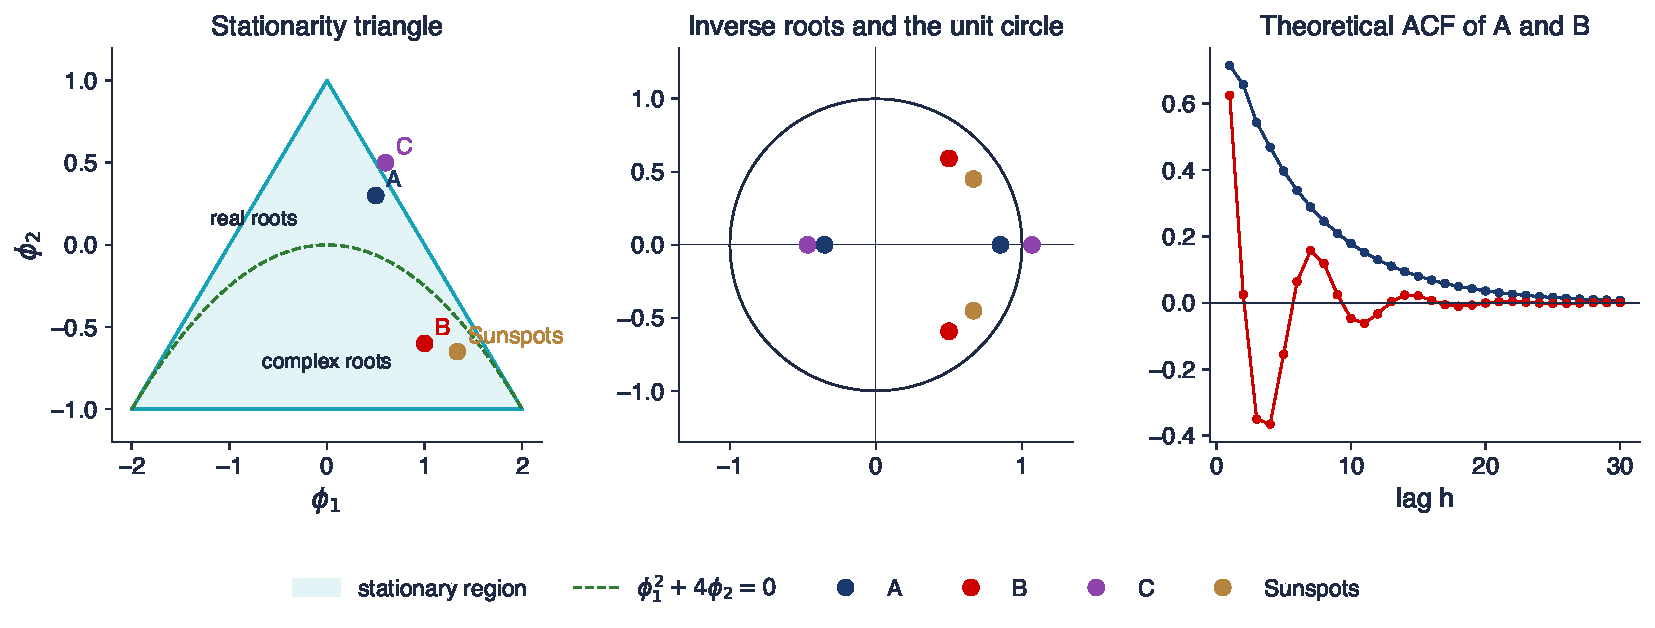
\includegraphics[width=0.97\textwidth,height=0.72\textheight,keepaspectratio]{tsa_ch2_ar2.pdf}
\end{center}
\vspace{-0.25cm}
\begin{itemize}
    \item A: $\phi = (0{,}5; 0{,}3)$; B: $(1{,}0; -0{,}6)$; C: $(0{,}6; 0{,}5)$; Sunspots: AR(2)-ul lui Yule, estimat în secțiunea 10
    \item Mijloc: rădăcinile inverse $\lambda_i$; staționar înseamnă în interiorul cercului
\end{itemize}
\quantlet{TSA\_ch2\_ar\_models}{\qlurl{TSA_ch2_ar_models}}
\end{frame}

\begin{frame}{Interpretarea exemplelor AR(2)}
\itemsize{\small}
\begin{itemize}
    \item \textbf{A}: rădăcini reale $-2{,}84$ și $1{,}17$, ambele în afara cercului: staționar
    \begin{itemize}
        \item $\rho(1) = 0{,}5/0{,}7 = 0{,}714$, $\rho(2) = 0{,}5\rho(1) + 0{,}3 = 0{,}657$: descreștere lentă și netedă
    \end{itemize}
    \item \textbf{B}: rădăcini complexe $0{,}833 \pm 0{,}986\,i$, modul $1{,}291 > 1$: staționar
    \begin{itemize}
        \item ACF: o undă cu perioada de 7{,}2 decalaje, amortizată cu $0{,}775$ pe decalaj: un \textbf{ciclu stochastic}
    \end{itemize}
    \item \textbf{C}: $\phi_1 + \phi_2 = 1{,}1 > 1$; o rădăcină $0{,}936 < 1$: proces \textbf{nestaționar} (exploziv)
    \begin{itemize}
        \item fiecare coeficient este sub 1, totuși procesul explodează: verificați întotdeauna rădăcinile, nu coeficienții unul cîte unul
    \end{itemize}
    \item Rădăcinile complexe sînt mecanismul prin care modelele liniare produc ciclurile economice și ciclul solar de 11 ani
\end{itemize}
\end{frame}

\begin{frame}{PACF a unui AR($p$) se anulează după decalajul $p$}
\itemsize{\small}
\begin{itemize}
    \item $\phi_{hh}$ = ultimul coeficient din cea mai bună predicție liniară a lui $X_t$ din $X_{t-1}, \dots, X_{t-h}$ (\tsachlink{https://danpele.github.io/Time-Series-Analysis/RO/Cursuri/capitol1_procese_stochastice_stationaritate.pdf}{Capitolul 1})
    \begin{itemize}
        \item calculat din ACF prin recursia Durbin--Levinson (\refDurbin)
    \end{itemize}
    \item Pentru un AR($p$) și $h > p$, cel mai bun predictor este chiar modelul: $\phi_1X_{t-1} + \dots + \phi_pX_{t-p}$
    \begin{itemize}
        \item deci $\phi_{hh} = 0$ pentru $h > p$, iar $\phi_{pp} = \phi_p$
    \end{itemize}
    \item \textbf{Regula de identificare}: ACF descrește treptat, PACF are $p$ valori semnificative și apoi rămîne în bandă: AR($p$)
    \begin{itemize}
        \item banda pentru PACF de selecție a unui AR($p$) la decalajele $h > p$: $\pm 1{,}96/\sqrt{T}$
    \end{itemize}
\end{itemize}
\end{frame}

\begin{frame}{Recapitulare: modele autoregresive}
\itemsize{\small}
\begin{itemize}
    \item AR($p$): $\phi(L)X_t = c + \varepsilon_t$; staționar dacă și numai dacă toate rădăcinile lui $\phi(z)$ sînt în afara cercului unitate
    \item Media $\mu = c/\phi(1)$; ACF din recurența Yule--Walker, o combinație de descreșteri geometrice și unde amortizate
    \item AR(1): $\rho(h) = \phi^h$, $\psi_j = \phi^j$, timpul de înjumătățire $\ln 0{,}5/\ln\phi$
    \item PACF se anulează după decalajul $p$: semnătura unui AR($p$)
\end{itemize}
\end{frame}


%=============================================================================
\section{Modele de medie mobilă}
%=============================================================================

\begin{frame}{Modelul MA($q$)}
\itemsize{\small}
\begin{itemize}
    \item $X_t = \mu + \theta(L)\varepsilon_t = \mu + \varepsilon_t + \theta_1\varepsilon_{t-1} + \dots + \theta_q\varepsilon_{t-q}$
    \begin{itemize}
        \item o sumă Wold finită: \textbf{întotdeauna staționar}, pentru orice $\theta$
    \end{itemize}
    \item Momentele (deduse în Seminarul 1 și în \tsachlink{https://danpele.github.io/Time-Series-Analysis/RO/Cursuri/capitol1_procese_stochastice_stationaritate.pdf}{Capitolul 1}): cu $\theta_0 = 1$
    \begin{itemize}
        \item $E[X_t] = \mu$; $\gamma(h) = \sigma^2\sum_{j=0}^{q-h}\theta_j\theta_{j+h}$ pentru $0 \le h \le q$; $\gamma(h) = 0$ pentru $h > q$
    \end{itemize}
    \item \textbf{Regula de identificare}: ACF \textbf{se anulează} după decalajul $q$; PACF descrește treptat
    \begin{itemize}
        \item imaginea în oglindă a regulii pentru AR($p$)
        \item banda pentru ACF de selecție la decalajele $h > q$ (Bartlett): $\pm 1{,}96\sqrt{(1 + 2\sum_{j=1}^{q}\hat\rho(j)^2)/T}$, mai largă decît $\pm 1{,}96/\sqrt{T}$
    \end{itemize}
\end{itemize}
\end{frame}

\begin{frame}{MA(1): $\theta = 0{,}8$ și $\theta = -0{,}8$}
\itemsize{\footnotesize}
\begin{center}
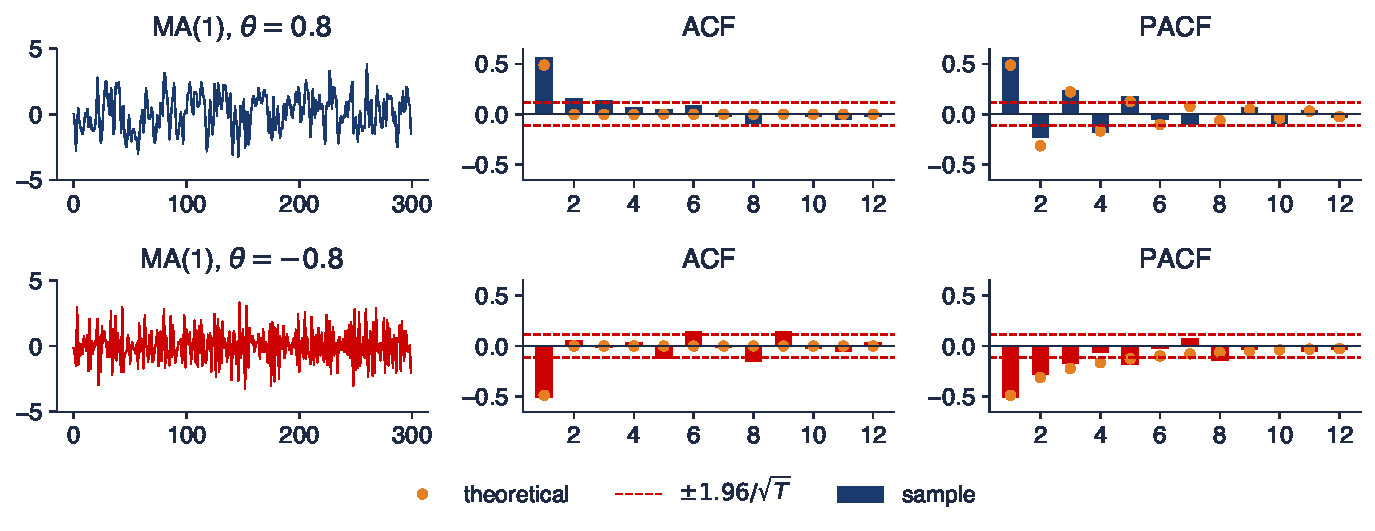
\includegraphics[width=0.97\textwidth,height=0.72\textheight,keepaspectratio]{tsa_ch2_ma1.pdf}
\end{center}
\vspace{-0.25cm}
\begin{itemize}
    \item $T = 300$; ACF are o singură valoare semnificativă, PACF descrește (cu semne alternante cînd $\theta > 0$)
\end{itemize}
\quantlet{TSA\_ch2\_ma\_models}{\qlurl{TSA_ch2_ma_models}}
\end{frame}

\begin{frame}{Interpretarea corelogramelor MA(1)}
\itemsize{\small}
\begin{itemize}
    \item Teoretic: $\rho(1) = \theta/(1 + \theta^2) = \pm 0{,}488$, $\rho(h) = 0$ pentru $h \ge 2$
    \begin{itemize}
        \item de selecție: $\hat\rho(1) = 0{,}56$ și $-0{,}51$
    \end{itemize}
    \item PACF nu se anulează: $\hat\phi_{22} = -0{,}23$ pentru $\theta = 0{,}8$
    \begin{itemize}
        \item un MA(1) este un AR($\infty$) (slide-urile următoare), deci fiecare valoare trecută ajută puțin
    \end{itemize}
    \item Un MA(1) își amintește exact o perioadă: un șoc de azi afectează ziua de mîine și apoi este uitat
    \item Exemple economice: observații care se suprapun (secțiunea 9), o eroare de măsurare, oscilația bid--ask a prețurilor
\end{itemize}
\end{frame}

\begin{frame}{Cea mai mare autocorelație a unui MA(1)}
\itemsize{\footnotesize}
\begin{center}
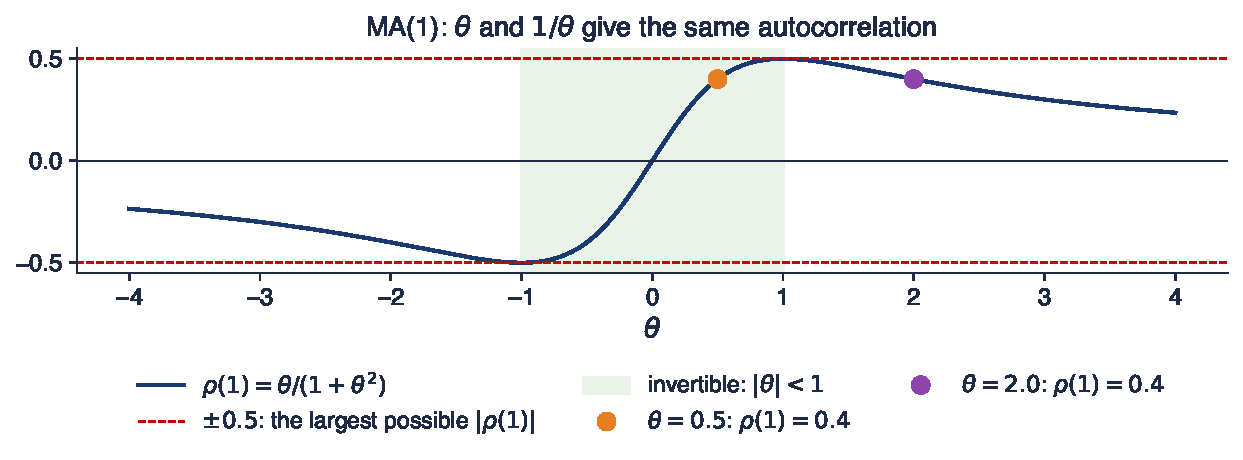
\includegraphics[width=0.97\textwidth,height=0.72\textheight,keepaspectratio]{tsa_ch2_ma1_rho.pdf}
\end{center}
\vspace{-0.25cm}
\begin{itemize}
    \item $\rho(1) = \theta/(1 + \theta^2)$ ca funcție de $\theta$
\end{itemize}
\quantlet{TSA\_ch2\_ma\_models}{\qlurl{TSA_ch2_ma_models}}
\end{frame}

\begin{frame}{Interpretarea curbei $\rho(1)$}
\itemsize{\small}
\begin{itemize}
    \item Maximul $|\rho(1)| = 0{,}5$ în $\theta = \pm 1$: un MA(1) nu poate produce niciodată $|\rho(1)| > 0{,}5$
    \begin{itemize}
        \item dacă $\hat\rho(1) = 0{,}7$ și apoi nimic: nu este un MA(1); încercați un AR sau un MA($q$) cu mai mulți termeni
    \end{itemize}
    \item $\theta = 0{,}5$ și $\theta = 2$ dau același $\rho(1) = 0{,}4$
    \begin{itemize}
        \item în general, $\theta$ și $1/\theta$ dau aceeași ACF (cu $\sigma^2$ înmulțit cu $\theta^2$)
        \item datele nu le pot deosebi: o \textbf{problemă de identificare}
    \end{itemize}
    \item Convenția care elimină ambiguitatea: invertibilitatea, $|\theta| < 1$ (slide-ul următor)
\end{itemize}
\end{frame}

\begin{frame}{Invertibilitatea}
\itemsize{\small}
\begin{itemize}
    \item MA(1): $\varepsilon_t = X_t - \theta\varepsilon_{t-1}$; substituim repetat ($\mu = 0$):
    \begin{itemize}
        \item $\varepsilon_t = X_t - \theta X_{t-1} + \theta^2X_{t-2} - \dots = \sum_{j \ge 0}(-\theta)^jX_{t-j}$, dacă $|\theta| < 1$
        \item o \textbf{reprezentare AR($\infty$)}: $X_t = \theta X_{t-1} - \theta^2X_{t-2} + \dots + \varepsilon_t$
    \end{itemize}
    \item \textbf{Invertibil}: șocurile pot fi recuperate din trecutul lui $X$; condiția: toate rădăcinile lui $\theta(z) = 0$ în afara cercului unitate
    \begin{itemize}
        \item MA(1): $|\theta| < 1$; aceeași algebră ca la staționaritatea AR, aplicată lui $\theta(z)$
    \end{itemize}
    \item De ce o dorim
    \begin{itemize}
        \item unicitate: dintre $\theta$ și $1/\theta$ doar unul este invertibil
        \item prognoză: șocurile $\varepsilon_t$ se calculează din date, deci prognozele le pot folosi
        \item programele raportează estimări invertibile; o rădăcină aproape de cerc semnalează supradiferențierea (\tsachlink{https://danpele.github.io/Time-Series-Analysis/RO/Cursuri/capitol1_procese_stochastice_stationaritate.pdf}{Capitolul 1})
    \end{itemize}
\end{itemize}
\end{frame}

\begin{frame}{Exemplu rezolvat: $\theta = 2$ sau $\theta = 0{,}5$?}
\itemsize{\small}
\begin{itemize}
    \item $X_t = \varepsilon_t + 2\varepsilon_{t-1}$, $\sigma^2 = 1$; și $Y_t = u_t + 0{,}5u_{t-1}$, $\mathrm{Var}(u_t) = 4$
    \item $X$: $\gamma(0) = 1 \cdot (1 + 4) = 5$, $\gamma(1) = 2 \cdot 1 = 2$
    \begin{itemize}
        \item $Y$: $\gamma(0) = 4 \cdot (1 + 0{,}25) = 5$, $\gamma(1) = 0{,}5 \cdot 4 = 2$
    \end{itemize}
    \item Aceeași medie, aceleași autocovarianțe: cu șocuri gaussiene, \textbf{aceeași distribuție}
    \begin{itemize}
        \item oricît de multe date am avea, nu le putem separa
    \end{itemize}
    \item Doar $Y$ este invertibil: $u_t = Y_t - 0{,}5Y_{t-1} + 0{,}25Y_{t-2} - \dots$
    \begin{itemize}
        \item pentru $X$, aceeași sumă cu ponderile $(-2)^j$ explodează
    \end{itemize}
    \item Regula: raportăm versiunea invertibilă ($\theta = 0{,}5$, $\sigma^2 = 4$)
\end{itemize}
\end{frame}

\begin{frame}{Recapitulare: modele de medie mobilă}
\itemsize{\small}
\begin{itemize}
    \item MA($q$) este întotdeauna staționar; ACF lui se anulează după decalajul $q$, PACF descrește
    \item MA(1): $\rho(1) = \theta/(1 + \theta^2)$, cel mult $0{,}5$ în valoare absolută
    \item Invertibil dacă și numai dacă rădăcinile lui $\theta(z)$ sînt în afara cercului unitate; atunci MA = AR($\infty$)
    \item $\theta$ și $1/\theta$ sînt echivalente observațional; îl păstrăm pe cel invertibil
\end{itemize}
\end{frame}


%=============================================================================
\section{Modele ARMA($p,q$)}
%=============================================================================

\begin{frame}{Modelul ARMA($p,q$)}
\itemsize{\small}
\begin{itemize}
    \item $\phi(L)(X_t - \mu) = \theta(L)\varepsilon_t$, adică
    \begin{itemize}
        \item $X_t = c + \phi_1X_{t-1} + \dots + \phi_pX_{t-p} + \varepsilon_t + \theta_1\varepsilon_{t-1} + \dots + \theta_q\varepsilon_{t-q}$, $c = \mu\,\phi(1)$
    \end{itemize}
    \item Trei condiții (\refBD, cap.~3)
    \begin{itemize}
        \item \textbf{staționar și cauzal}: rădăcinile lui $\phi(z)$ în afara cercului unitate; atunci $X_t - \mu = \psi(L)\varepsilon_t$, $\psi(L) = \theta(L)/\phi(L)$
        \item \textbf{invertibil}: rădăcinile lui $\theta(z)$ în afara cercului unitate; atunci $\pi(L)(X_t - \mu) = \varepsilon_t$, $\pi(L) = \phi(L)/\theta(L)$
        \item \textbf{fără factori comuni}: $\phi(z)$ și $\theta(z)$ nu au nicio rădăcină comună
    \end{itemize}
    \item ARMA(1,1) poate reproduce o ACF care descrește lent și pornește sub $\phi$; un AR sau un MA pur ar avea nevoie de mulți termeni
\end{itemize}
\end{frame}

\begin{frame}{Ponderile $\psi$ și răspunsul la impuls}
\itemsize{\small}
\begin{itemize}
    \item Din $\phi(L)\psi(L) = \theta(L)$, egalăm coeficienții lui $L^j$:
    \begin{itemize}
        \item $\psi_0 = 1$, \quad $\psi_j = \theta_j + \sum_{i=1}^{\min(j,p)}\phi_i\psi_{j-i}$ \quad ($\theta_j = 0$ pentru $j > q$)
    \end{itemize}
    \item ARMA(1,1): $\psi_1 = \phi + \theta$, $\psi_j = \phi^{j-1}(\phi + \theta)$ pentru $j \ge 1$
    \begin{itemize}
        \item exemplu $\phi = 0{,}7$, $\theta = 0{,}4$: $\psi_1 = 1{,}10$, $\psi_2 = 0{,}77$
    \end{itemize}
    \item \textbf{Răspunsul la impuls}: $\psi_j = \partial X_{t+j}/\partial\varepsilon_t$, efectul unui șoc unitar după $j$ perioade
    \begin{itemize}
        \item același obiect determină erorile de prognoză (secțiunea 7) și răspunsurile la impuls din modelele VAR (\tsachlink{https://danpele.github.io/Time-Series-Analysis/RO/Cursuri/capitol6_modele_var_cauzalitate_granger.pdf}{Capitolul 6})
    \end{itemize}
\end{itemize}
\end{frame}

\begin{frame}{Răspunsurile la impuls ale a patru modele}
\itemsize{\footnotesize}
\begin{center}
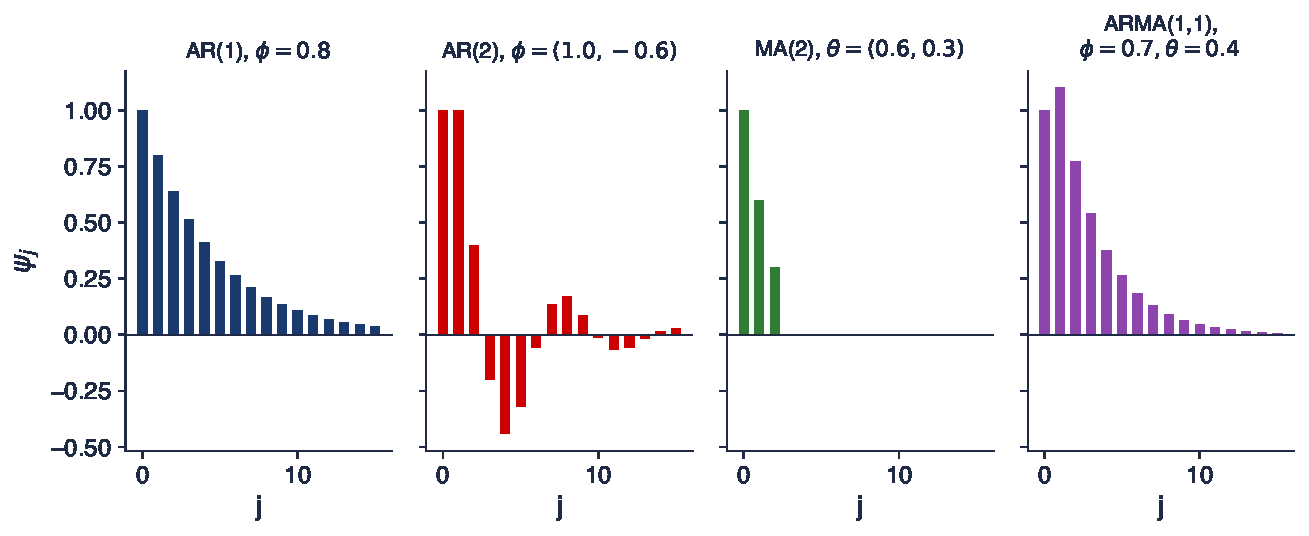
\includegraphics[width=0.97\textwidth,height=0.72\textheight,keepaspectratio]{tsa_ch2_psi.pdf}
\end{center}
\vspace{-0.25cm}
\begin{itemize}
    \item $\psi_j$, $j = 0, \dots, 15$, din recurența de mai sus
\end{itemize}
\quantlet{TSA\_ch2\_arma\_acf}{\qlurl{TSA_ch2_arma_acf}}
\end{frame}

\begin{frame}{Interpretarea răspunsurilor la impuls}
\itemsize{\small}
\begin{itemize}
    \item AR(1): descreștere geometrică $0{,}8^j$; șocul nu dispare niciodată complet, dar se stinge suficient de repede pentru ca $\sum\psi_j^2 < \infty$
    \item AR(2) cu rădăcini complexe: răspunsul își schimbă semnul, $\psi_3 = -0{,}20$, $\psi_4 = -0{,}44$: un șoc creează un ciclu
    \item MA(2): exact zero după două perioade: memorie finită
    \item ARMA(1,1): termenul MA ridică primul răspuns la $\psi_1 = 1{,}10 > 1$; după aceea preia partea AR
\end{itemize}
\end{frame}

\begin{frame}{Momentele procesului ARMA(1,1)}
\itemsize{\small}
\begin{itemize}
    \item $X_t = \phi X_{t-1} + \varepsilon_t + \theta\varepsilon_{t-1}$, $|\phi| < 1$, $|\theta| < 1$, $\phi + \theta \ne 0$
    \item Varianța, din $\gamma(0) = \sigma^2\sum_j\psi_j^2$:
    \begin{itemize}
        \item $\gamma(0) = \sigma^2\,\dfrac{1 + 2\phi\theta + \theta^2}{1 - \phi^2}$; pentru $\phi = 0{,}7$, $\theta = 0{,}4$, $\sigma^2 = 1$: $3{,}37$
    \end{itemize}
    \item Autocorelațiile:
    \begin{itemize}
        \item $\rho(1) = \dfrac{(1 + \phi\theta)(\phi + \theta)}{1 + 2\phi\theta + \theta^2}$, \quad $\rho(h) = \phi\,\rho(h - 1)$ pentru $h \ge 2$
        \item exemplu: $\rho(1) = 0{,}819$, $\rho(2) = 0{,}573$
    \end{itemize}
    \item ACF descrește ca la un AR(1) începînd cu decalajul 1, dar $\rho(1) \ne \phi$: partea MA mută doar punctul de pornire
\end{itemize}
\end{frame}

\begin{frame}{Factori comuni: un model prea mare}
\itemsize{\small}
\begin{itemize}
    \item $X_t = 0{,}5X_{t-1} + \varepsilon_t - 0{,}5\varepsilon_{t-1}$
    \begin{itemize}
        \item $(1 - 0{,}5L)X_t = (1 - 0{,}5L)\varepsilon_t$: simplificăm factorul, $X_t = \varepsilon_t$, zgomot alb
    \end{itemize}
    \item În general, $\phi = -\theta$ într-un ARMA(1,1) dă zgomot alb, pentru orice valoare
    \begin{itemize}
        \item verosimilitatea este plată de-a lungul dreptei $\phi = -\theta$: parametrii nu sînt identificați
    \end{itemize}
    \item Simptome în rezultatele programelor
    \begin{itemize}
        \item estimări mari și de semne opuse, de exemplu $\hat\phi = 0{,}9$, $\hat\theta = -0{,}88$, cu erori standard foarte mari
        \item o log-verosimilitate care nu este mai bună decît a modelului mai mic
    \end{itemize}
    \item Remediul: reducem $p$ și $q$ împreună; preferăm cel mai mic model cu reziduuri de tip zgomot alb
\end{itemize}
\end{frame}

\begin{frame}{Identificarea: tabelul ACF--PACF}
\itemsize{\small}
\begin{center}
\footnotesize
\begin{tabular}{lll}
\toprule
\textbf{Modelul} & \textbf{ACF} & \textbf{PACF} \\
\midrule
Zgomot alb & niciun decalaj semnificativ & niciun decalaj semnificativ \\
AR($p$) & descrește (geometric sau undă amortizată) & \textbf{se anulează} după decalajul $p$ \\
MA($q$) & \textbf{se anulează} după decalajul $q$ & descrește \\
ARMA($p,q$) & descrește după decalajul $q - p$ & descrește după decalajul $p - q$ \\
Rădăcină unitară (cap.~3) & descreștere foarte lentă, aproape liniară & $\hat\phi_{11} \approx 1$ \\
\bottomrule
\end{tabular}
\end{center}
\begin{itemize}
    \item Tabelul propune \textbf{candidați}; criteriile informaționale și diagnosticarea decid (secțiunile 5--6)
    \item Modelele ARMA mixte sînt greu de recunoscut din ochi: ambele funcții doar descresc
\end{itemize}
\end{frame}

\begin{frame}{ACF și PACF teoretice și de selecție}
\itemsize{\footnotesize}
\begin{center}
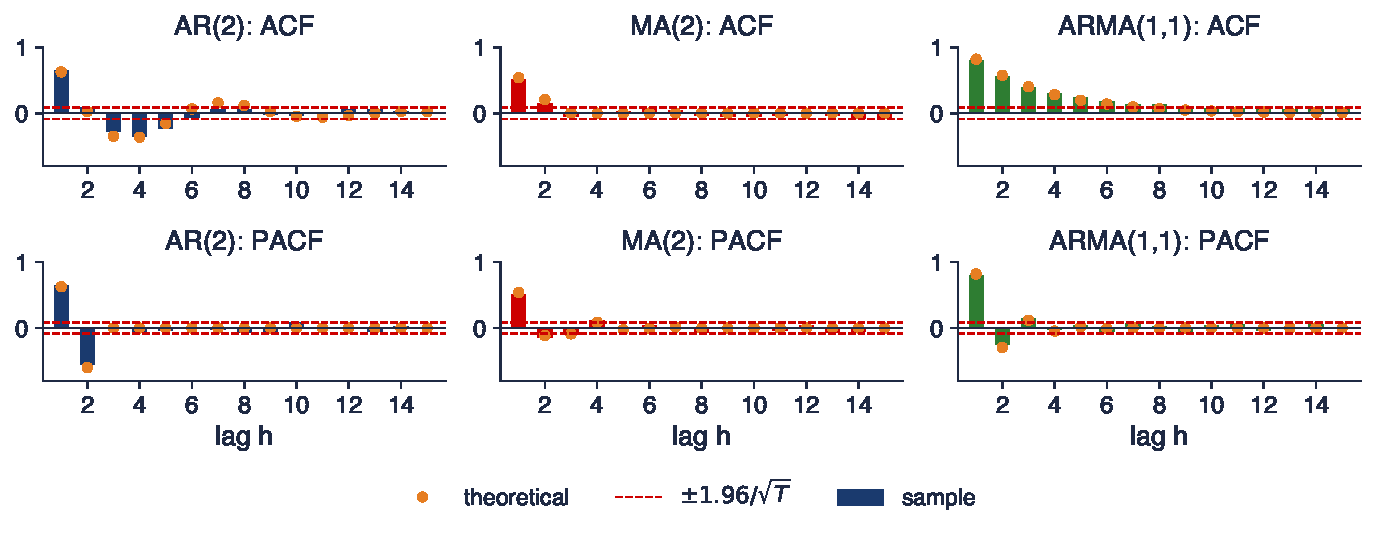
\includegraphics[width=0.97\textwidth,height=0.72\textheight,keepaspectratio]{tsa_ch2_patterns.pdf}
\end{center}
\vspace{-0.25cm}
\begin{itemize}
    \item AR(2) $\phi = (1{,}0; -0{,}6)$, MA(2) $\theta = (0{,}6; 0{,}3)$, ARMA(1,1) $\phi = 0{,}7$, $\theta = 0{,}4$; cîte o traiectorie simulată cu $T = 500$
\end{itemize}
\quantlet{TSA\_ch2\_arma\_acf}{\qlurl{TSA_ch2_arma_acf}}
\end{frame}

\begin{frame}{Interpretarea celor trei tipare}
\itemsize{\small}
\begin{itemize}
    \item AR(2): PACF are două valori semnificative, $\phi_{22} = \phi_2 = -0{,}60$, apoi zero; ACF este o undă amortizată
    \begin{itemize}
        \item identificarea este ușoară: citim $p$ din PACF
    \end{itemize}
    \item MA(2): $\rho(1) = 0{,}538$, $\rho(2) = 0{,}207$, apoi zero; PACF descrește lent
    \begin{itemize}
        \item ACF de selecție la decalajul 2 iese abia ușor din bandă: pe date reale, MA(1) și MA(2) pot semăna
    \end{itemize}
    \item ARMA(1,1): ambele descresc; ACF seamănă cu un AR(1), PACF are o a doua valoare, mai mică
    \begin{itemize}
        \item un analist care citește doar PACF ar alege AR(2) sau AR(3): apropiat, dar cu mai mulți parametri
    \end{itemize}
    \item Corelogramele de selecție sînt zgomotoase chiar cu $T = 500$; cu 100 de observații trimestriale, mult mai mult
\end{itemize}
\end{frame}

\begin{frame}{Recapitulare: modele ARMA}
\itemsize{\small}
\begin{itemize}
    \item ARMA($p,q$): $\phi(L)(X_t - \mu) = \theta(L)\varepsilon_t$; cauzal dacă $\phi(z)$ are rădăcinile în afara cercului, invertibil dacă $\theta(z)$ le are
    \item Ponderile $\psi$ prin recurența $\psi_j = \theta_j + \sum\phi_i\psi_{j-i}$: răspunsul la impuls
    \item Fără factori comuni; o verosimilitate plată și estimări opuse semnalează unul
    \item ACF se anulează: MA; PACF se anulează: AR; ambele descresc: ARMA
\end{itemize}
\end{frame}


%=============================================================================
\section{Estimarea}
%=============================================================================

\begin{frame}{Trei estimatori}
\itemsize{\small}
\begin{itemize}
    \item \textbf{Yule--Walker} (metoda momentelor, \refYule; \refWalker): înlocuim $\rho(h)$ cu $\hat\rho(h)$ în ecuațiile Yule--Walker
    \begin{itemize}
        \item doar pentru AR pur; rapid; dă întotdeauna un model staționar; mai puțin precis cînd rădăcinile sînt aproape de cerc
    \end{itemize}
    \item \textbf{Cele mai mici pătrate condiționate}: minimizăm $\sum_t\varepsilon_t^2$, tratînd primele valori ca fixe
    \begin{itemize}
        \item AR($p$): metoda celor mai mici pătrate (OLS) pentru $X_t$ pe $1, X_{t-1}, \dots, X_{t-p}$
        \item MA și ARMA: reziduurile $\varepsilon_t = X_t - \mu - \theta\varepsilon_{t-1} - \dots$ se calculează recursiv, pornind de la $\varepsilon_0 = 0$; minimizare numerică
    \end{itemize}
    \item \textbf{Verosimilitatea maximă exactă gaussiană} (MLE): maximizăm densitatea comună a lui $(X_1, \dots, X_T)$
    \begin{itemize}
        \item folosește și primele observații; metoda implicită a lui \texttt{ARIMA} din \texttt{statsmodels} (filtrul Kalman, \tsachlink{https://danpele.github.io/Time-Series-Analysis/RO/Cursuri/capitol10_spatiul_starilor_kalman_markov_switching.pdf}{Capitolul 10})
    \end{itemize}
    \item În eșantioane mari, cele trei coincid pentru modelele AR pure; MLE este referința pentru MA și ARMA
\end{itemize}
\end{frame}

\begin{frame}{Yule--Walker pentru un AR($p$)}
\itemsize{\footnotesize}
\begin{columns}[T]
\begin{column}{0.64\textwidth}
\begin{itemize}
    \item Pentru $h = 1, \dots, p$: $\rho(h) = \phi_1\rho(h - 1) + \dots + \phi_p\rho(h - p)$
    \begin{itemize}
        \item matricial, $R\,\phi = \rho$, $R_{ij} = \rho(|i - j|)$
        \item estimatorul $\hat\phi = \hat R^{-1}\hat\rho$; varianța zgomotului $\hat\sigma^2 = \hat\gamma(0)(1 - \hat\phi^\top\hat\rho)$
    \end{itemize}
    \item AR(2) prin regula lui Cramer:
    \begin{itemize}
        \item $\hat\phi_1 = \dfrac{\hat\rho_1(1 - \hat\rho_2)}{1 - \hat\rho_1^2}$, \quad $\hat\phi_2 = \dfrac{\hat\rho_2 - \hat\rho_1^2}{1 - \hat\rho_1^2}$
        \item $\hat\phi_2$ este PACF de selecție la decalajul 2 (\tsachlink{https://danpele.github.io/Time-Series-Analysis/RO/Cursuri/capitol1_procese_stochastice_stationaritate.pdf}{Capitolul 1})
    \end{itemize}
\end{itemize}
\end{column}
\begin{column}{0.32\textwidth}
\centering
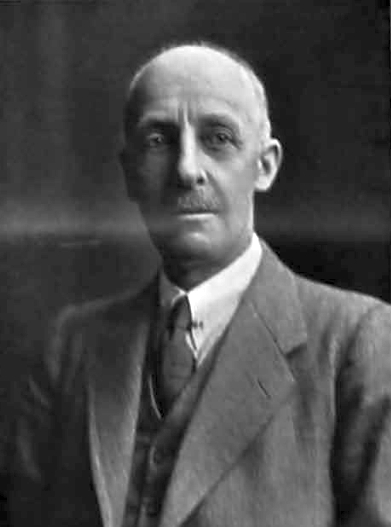
\includegraphics[height=0.46\textheight]{ch2_gilbert_walker.jpg}\\[1mm]
\imgcap{Gilbert Walker (1868--1958), care a extins metoda lui Yule în 1931}
\imgcredit{https://commons.wikimedia.org/wiki/File:Gilbert_Walker.jpg}{Foto: autor necunoscut (1925); domeniu public; Wikimedia Commons}
\end{column}
\end{columns}
\end{frame}

\begin{frame}{Exemplu rezolvat: Yule--Walker pentru creșterea PIB-ului României}
\itemsize{\footnotesize}
\begin{itemize}
    \item Creșterea anuală a PIB-ului real, T1 2000--T2 2026 (secțiunea 9): $\hat\rho(1) = 0{,}62$, $\hat\rho(2) = 0{,}40$, $\hat\gamma(0) = 18{,}95$
    \item Determinantul $1 - \hat\rho_1^2 = 0{,}620$
    \begin{itemize}
        \item $\hat\phi_1 = 0{,}62\,(1 - 0{,}40)/0{,}620 = 0{,}600$
        \item $\hat\phi_2 = (0{,}40 - 0{,}62^2)/0{,}620 = 0{,}027$
    \end{itemize}
    \item $\hat\sigma^2 = 18{,}95\,(1 - \hat\phi_1\hat\rho_1 - \hat\phi_2\hat\rho_2) = 11{,}74$
    \item $\hat\phi_2 \approx 0$: al doilea decalaj nu aduce nimic, AR(1) ar fi suficient
    \begin{itemize}
        \item dar este familia AR cea potrivită? Secțiunea 9 arată că un MA(3) se potrivește mai bine
    \end{itemize}
\end{itemize}
\end{frame}

\begin{frame}{Verosimilitatea maximă}
\itemsize{\small}
\begin{itemize}
    \item Verosimilitatea gaussiană prin \textbf{descompunerea erorilor de predicție}
    \begin{itemize}
        \item $f(x_1, \dots, x_T) = \prod_t f(x_t \mid x_{t-1}, \dots, x_1)$; fiecare factor este $N(\hat x_{t|t-1}, v_t)$
        \item $\ln L = -\tfrac12\sum_{t=1}^{T}\big[\ln(2\pi v_t) + (x_t - \hat x_{t|t-1})^2/v_t\big]$
        \item $\hat x_{t|t-1}$: predicția cu un pas; $v_t$: varianța erorii ei, mai mare pentru primele observații
    \end{itemize}
    \item AR(1) de mînă: $X_1 \sim N(\mu, \sigma^2/(1 - \phi^2))$, apoi $X_t \mid X_{t-1} \sim N(c + \phi X_{t-1}, \sigma^2)$
    \begin{itemize}
        \item dacă renunțăm la primul factor, obținem cele mai mici pătrate condiționate
    \end{itemize}
    \item Erorile standard din curbura lui $\ln L$; asimptotic
    \begin{itemize}
        \item AR(1): $\mathrm{se}(\hat\phi) \approx \sqrt{(1 - \phi^2)/T}$; MA(1): $\mathrm{se}(\hat\theta) \approx \sqrt{(1 - \theta^2)/T}$
        \item rapoartele $t$, $\hat\phi/\mathrm{se}$, se compară cu $\pm 1{,}96$, ca în regresie
    \end{itemize}
\end{itemize}
\end{frame}

\begin{frame}{Distribuțiile de selecție ale estimatorilor}
\itemsize{\footnotesize}
\begin{center}
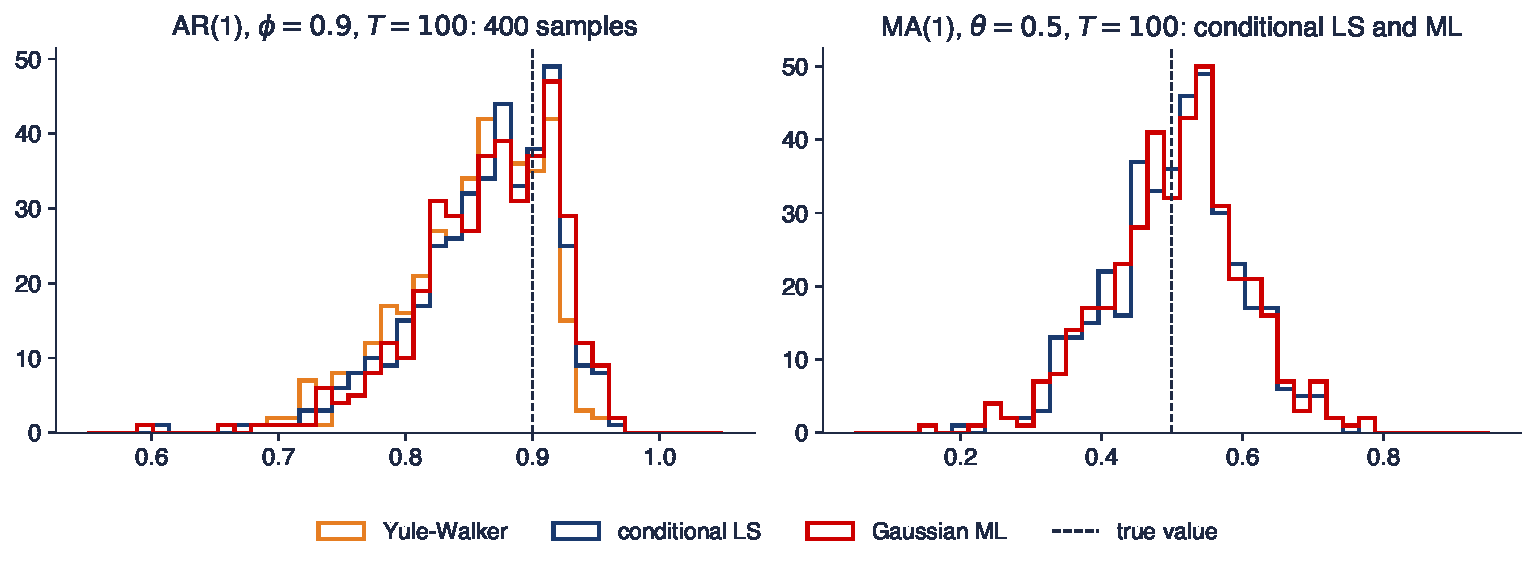
\includegraphics[width=0.97\textwidth,height=0.72\textheight,keepaspectratio]{tsa_ch2_estimators.pdf}
\end{center}
\vspace{-0.25cm}
\begin{itemize}
    \item 400 de eșantioane simulate, fiecare cu $T = 100$; stînga: AR(1) cu $\phi = 0{,}9$; dreapta: MA(1) cu $\theta = 0{,}5$
\end{itemize}
\quantlet{TSA\_ch2\_estimation}{\qlurl{TSA_ch2_estimation}}
\end{frame}

\begin{frame}{Interpretarea comparației estimatorilor}
\itemsize{\small}
\begin{itemize}
    \item AR(1), $\phi = 0{,}9$: mediile 0{,}853 (Yule--Walker), 0{,}864 (cele mai mici pătrate condiționate), 0{,}866 (MLE)
    \begin{itemize}
        \item toți trei sînt deplasați în jos; aproximarea de manual a deplasării celor mai mici pătrate este $-(1 + 3\phi)/T = -0{,}037$
        \item Yule--Walker este cel mai deplasat aproape de cercul unitate
    \end{itemize}
    \item Abaterile standard 0{,}056; 0{,}055; 0{,}054, peste valoarea asimptotică 0{,}044
    \begin{itemize}
        \item distribuția este asimetrică la stînga: intervalele asimptotice sînt optimiste aproape de $\phi = 1$
    \end{itemize}
    \item MA(1), $\theta = 0{,}5$: cele mai mici pătrate condiționate 0{,}504 (abaterea standard 0{,}097), MLE 0{,}506 (0{,}098); valoarea asimptotică 0{,}087
    \item Regula practică: folosiți MLE; Yule--Walker doar pentru valori de pornire rapide sau în scop didactic
\end{itemize}
\end{frame}

\begin{frame}{Recapitulare: estimarea}
\itemsize{\small}
\begin{itemize}
    \item Yule--Walker: momente, AR pur, $\hat\phi = \hat R^{-1}\hat\rho$
    \item Cele mai mici pătrate condiționate: OLS pentru AR, o recurență pentru MA
    \item MLE exactă gaussiană: descompunerea erorilor de predicție; standardul programelor
    \item Coeficienții AR persistenți sînt deplasați în jos în eșantioane mici
\end{itemize}
\end{frame}


%=============================================================================
\section{Selecția modelului și diagnosticarea}
%=============================================================================

\begin{frame}{Criterii informaționale}
\itemsize{\footnotesize}
\begin{columns}[T]
\begin{column}{0.64\textwidth}
\begin{itemize}
    \item Ajustarea se îmbunătățește cu fiecare parametru; criteriile impun o \textbf{penalizare} pe parametru
    \begin{itemize}
        \item $k$ = numărul parametrilor estimați ($\phi$, $\theta$, $\mu$, $\sigma^2$), $\ln L$ = log-verosimilitatea maximizată
    \end{itemize}
    \item \textbf{AIC} $= -2\ln L + 2k$ (\refAkaike)
    \begin{itemize}
        \item \textbf{AICc} $= \mathrm{AIC} + 2k(k + 1)/(T - k - 1)$, pentru $T$ mic (\refHT)
    \end{itemize}
    \item \textbf{BIC} $= -2\ln L + k\ln T$ (\refSchwarz)
    \begin{itemize}
        \item $\ln T > 2$ de îndată ce $T \ge 8$: BIC preferă modele mai mici
    \end{itemize}
    \item Alegem modelul cu valoarea \textbf{cea mai mică}; comparăm doar modele estimate pe aceleași observații
\end{itemize}
\end{column}
\begin{column}{0.32\textwidth}
\centering
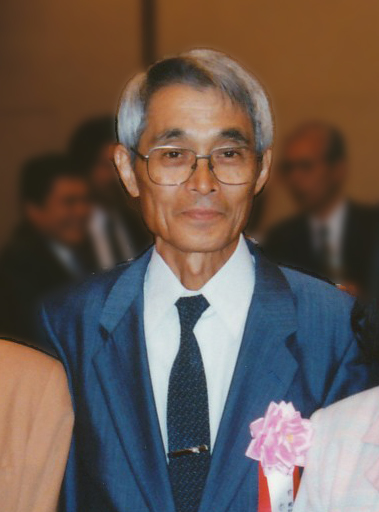
\includegraphics[height=0.44\textheight]{ch2_hirotugu_akaike.jpg}\\[1mm]
\imgcap{Hirotugu Akaike (1927--2009), Institutul de Matematică Statistică, Tokyo}
\imgcredit{https://commons.wikimedia.org/wiki/File:Akaike.jpg}{Foto: The Institute of Statistical Mathematics (2017); CC BY-SA 4.0; Wikimedia Commons}
\end{column}
\end{columns}
\end{frame}

\begin{frame}{AIC sau BIC?}
\itemsize{\small}
\begin{itemize}
    \item \textbf{BIC este consistent}: dacă modelul adevărat se află printre candidați, BIC îl găsește cu probabilitate $\to 1$
    \begin{itemize}
        \item dar poate alege un model prea mic cînd $T$ este mic
    \end{itemize}
    \item \textbf{AIC țintește prognoza}: estimează ajustarea așteptată în afara eșantionului (distanța Kullback--Leibler)
    \begin{itemize}
        \item supraparametrizează cu probabilitate pozitivă, chiar pentru $T$ mare
    \end{itemize}
    \item Practica (\refFPP, cap.~9; \refHK)
    \begin{itemize}
        \item căutările automate (\texttt{auto.arima}, \texttt{pmdarima}) minimizează AICc pe o grilă de valori $(p, q)$
        \item cînd AIC și BIC nu coincid, păstrăm ambii candidați și lăsăm diagnosticarea și prognozele să decidă
    \end{itemize}
\end{itemize}
\end{frame}

\begin{frame}{Cît de des găsesc AIC și BIC ordinul adevărat}
\itemsize{\footnotesize}
\begin{center}
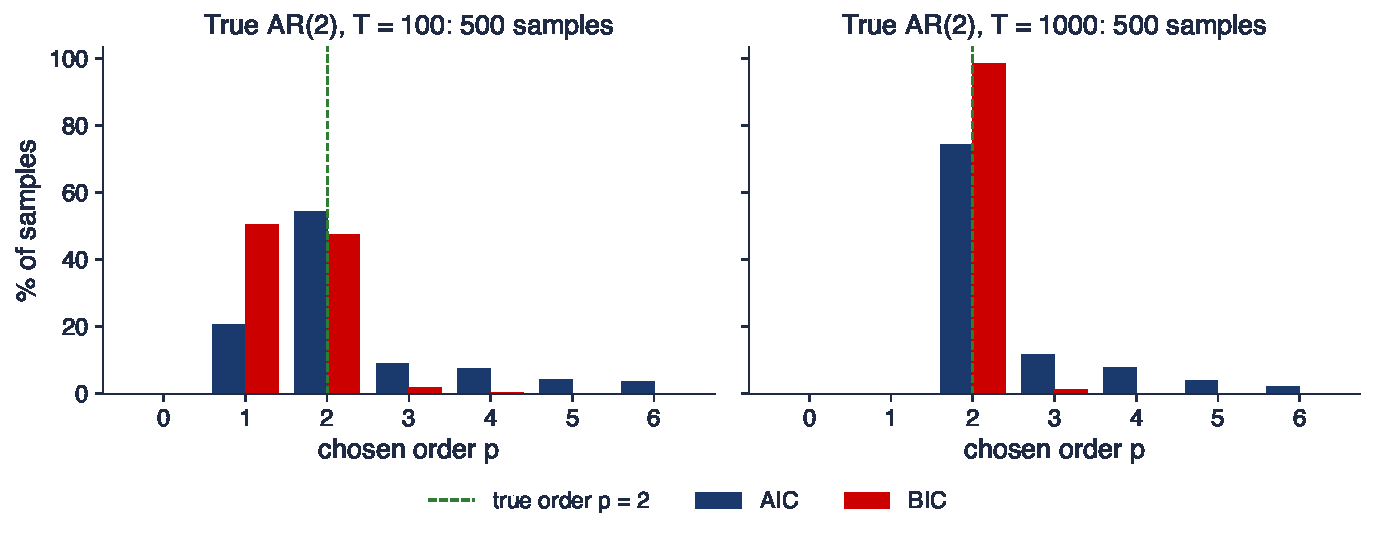
\includegraphics[width=0.97\textwidth,height=0.72\textheight,keepaspectratio]{tsa_ch2_ic.pdf}
\end{center}
\vspace{-0.25cm}
\begin{itemize}
    \item Modelul adevărat AR(2), $\phi = (0{,}5; 0{,}25)$; AR($p$), $p = 0, \dots, 6$, estimate prin OLS pe același eșantion; 500 de eșantioane pe panou
\end{itemize}
\quantlet{TSA\_ch2\_selection}{\qlurl{TSA_ch2_selection}}
\end{frame}

\begin{frame}{Interpretarea experimentului de selecție}
\itemsize{\small}
\begin{itemize}
    \item $T = 100$: AIC găsește $p = 2$ în 54{,}4\% din eșantioane, BIC în 47{,}4\%
    \begin{itemize}
        \item BIC alege un model prea mic în 50{,}4\% din cazuri (valoarea mică $\phi_2 = 0{,}25$ este greu de detectat); AIC alege unul prea mare în 24{,}8\%
    \end{itemize}
    \item $T = 1000$: BIC 98{,}6\%, AIC 74{,}4\%
    \begin{itemize}
        \item BIC este consistent; AIC încă supraparametrizează în 25{,}6\% din eșantioane
    \end{itemize}
    \item Niciun criteriu nu este o dovadă: cu date macroeconomice trimestriale ($T \approx 100$), ordinul este incert
    \item Supraparametrizarea costă puțin în prognoză; un model prea mic lasă corelație în reziduuri, pe care o detectează diagnosticarea
\end{itemize}
\end{frame}

\begin{frame}{Diagnosticarea reziduurilor}
\itemsize{\small}
\begin{itemize}
    \item Dacă modelul este corect, reziduurile $\hat\varepsilon_t$ se comportă ca un zgomot alb
    \begin{itemize}
        \item le reprezentăm grafic: fără tipare, fără schimbări de varianță, fără valori izolate foarte mari
        \item ACF a reziduurilor în banda $\pm 1{,}96/\sqrt{T}$, cu excepția a aproximativ 1 decalaj din 20
    \end{itemize}
    \item \textbf{Ljung--Box} pentru reziduuri (\refLB): $Q^*(m) = T(T + 2)\sum_{h=1}^{m}\hat\rho_{\hat\varepsilon}(h)^2/(T - h)$
    \begin{itemize}
        \item în ipoteza $H_0$ (model corect), $Q^*(m) \approx \chi^2(m - p - q)$ (\refBP): estimarea a $p + q$ coeficienți consumă $p + q$ grade de libertate
        \item alegem $m$ mult peste $p + q$: $m = 10$ pentru date anuale sau trimestriale, $m = 2s$ pentru date sezoniere (\refFPP)
    \end{itemize}
    \item \textbf{Normalitatea}: Jarque--Bera (\refJB) $\mathrm{JB} = \frac{T}{6}\big(S^2 + (K - 3)^2/4\big) \approx \chi^2(2)$; graficul QQ
    \begin{itemize}
        \item $S$ = asimetria, $K$ = boltirea; reziduurile ne-normale nu deplasează $\hat\phi$, dar fac greșite intervalele construite cu distribuția Normală
    \end{itemize}
    \item \textbf{Pătratele reziduurilor}: testul Ljung--Box pentru $\hat\varepsilon_t^2$ detectează volatility clustering (\tsachlink{https://danpele.github.io/Time-Series-Analysis/RO/Cursuri/capitol5_volatilitate_conditionata_garch.pdf}{Capitolul 5})
\end{itemize}
\end{frame}

\begin{frame}{Justificarea celor $m - p - q$ grade de libertate}
\itemsize{\footnotesize}
\begin{center}
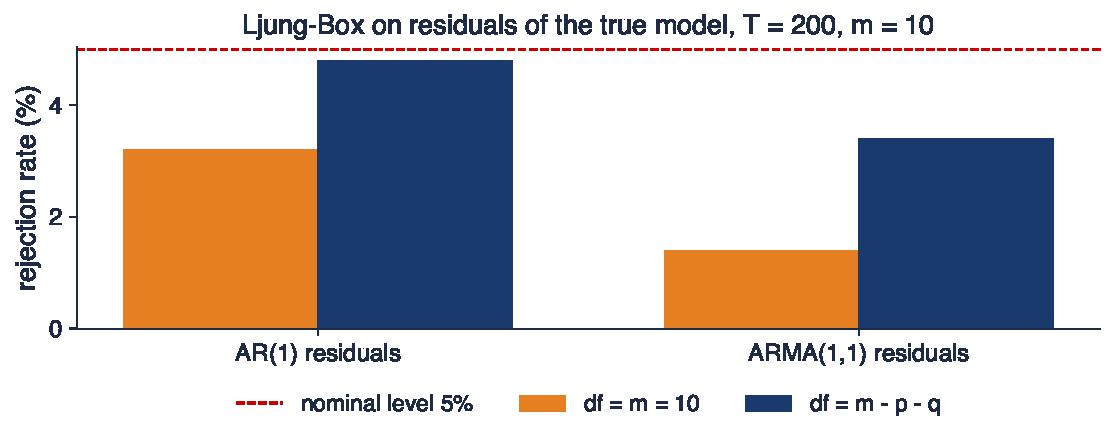
\includegraphics[width=0.97\textwidth,height=0.72\textheight,keepaspectratio]{tsa_ch2_lb_df.pdf}
\end{center}
\vspace{-0.25cm}
\begin{itemize}
    \item Testul Ljung--Box la 5\% pentru reziduurile modelului \textbf{adevărat}; 1\,000 de eșantioane AR(1), jumătate pentru ARMA(1,1)
\end{itemize}
\quantlet{TSA\_ch2\_selection}{\qlurl{TSA_ch2_selection}}
\end{frame}

\begin{frame}{Interpretarea experimentului cu gradele de libertate}
\itemsize{\small}
\begin{itemize}
    \item Cu $m = 10$ grade de libertate testul respinge prea rar: 3{,}2\% (AR(1)) și 1{,}4\% (ARMA(1,1)) în loc de 5\%
    \begin{itemize}
        \item reziduurile sînt ajustate astfel încît să pară necorelate la primele decalaje: ACF lor este mai mică decît a unui zgomot alb adevărat
    \end{itemize}
    \item Cu $m - p - q$: 4{,}8\% și 3{,}4\%, aproape de nivelul nominal de 5\%
    \begin{itemize}
        \item corecția contează cel mai mult cînd $p + q$ este mare în raport cu $m$
    \end{itemize}
    \item Programele (\texttt{acorr\_ljungbox}) folosesc implicit $m$: transmiteți \texttt{model\_df = p + q}
    \item Gradele de libertate greșite fac ca un model prost să pară acceptabil
\end{itemize}
\end{frame}

\begin{frame}{Recapitulare: selecția modelului și diagnosticarea}
\itemsize{\small}
\begin{itemize}
    \item AIC $= -2\ln L + 2k$, BIC $= -2\ln L + k\ln T$; cîștigă valoarea cea mai mică; BIC alege modele mai mici
    \item BIC este consistent, AIC țintește prognoza și uneori supraparametrizează
    \item Reziduurile: grafic, ACF, Ljung--Box cu $m - p - q$ grade de libertate, Jarque--Bera, Ljung--Box pe pătrate
    \item Un model este acceptat cînd reziduurile lui sînt zgomot alb; normalitatea contează pentru intervale
\end{itemize}
\end{frame}


%=============================================================================
\section{Prognoza cu modele ARMA}
%=============================================================================

\begin{frame}{Prognoza optimă}
\itemsize{\small}
\begin{itemize}
    \item Prognoza lui $X_{T+h}$ făcută la momentul $T$: $\hat X_{T+h|T} = E[X_{T+h} \mid X_T, X_{T-1}, \dots]$
    \begin{itemize}
        \item minimizează eroarea pătratică medie (MSE) între toate funcțiile de trecut
    \end{itemize}
    \item Rețeta: scriem modelul la $T + h$ și înlocuim
    \begin{itemize}
        \item șocurile viitoare $\varepsilon_{T+j}$, $j \ge 1$, cu 0
        \item valorile viitoare $X_{T+j}$ cu prognozele lor; valorile trecute și reziduurile trecute rămîn neschimbate
    \end{itemize}
    \item AR(1): $\hat X_{T+h|T} = \mu + \phi^h(X_T - \mu)$: \textbf{revenirea la medie} cu viteza $\phi$
    \begin{itemize}
        \item MA($q$): $\hat X_{T+h|T} = \mu$ pentru $h > q$: după $q$ pași modelul nu mai știe nimic în afară de medie
    \end{itemize}
\end{itemize}
\end{frame}

\begin{frame}{Erorile de prognoză și intervalele}
\itemsize{\small}
\begin{itemize}
    \item Din forma cauzală $X_{T+h} = \mu + \sum_j\psi_j\varepsilon_{T+h-j}$:
    \begin{itemize}
        \item eroarea $e_{T+h} = X_{T+h} - \hat X_{T+h|T} = \varepsilon_{T+h} + \psi_1\varepsilon_{T+h-1} + \dots + \psi_{h-1}\varepsilon_{T+1}$
        \item varianța $\sigma_h^2 = \sigma^2(1 + \psi_1^2 + \dots + \psi_{h-1}^2)$, crescătoare în $h$
    \end{itemize}
    \item \textbf{Intervalul de 95\%}: $\hat X_{T+h|T} \pm 1{,}96\,\sigma_h$ (șocuri gaussiene)
    \begin{itemize}
        \item $h = 1$: $\pm 1{,}96\,\sigma$; $h \to \infty$: $\sigma_h^2 \to \gamma(0)$, varianța necondiționată
    \end{itemize}
    \item Ce nu include intervalul
    \begin{itemize}
        \item incertitudinea parametrilor ($\hat\phi$ în loc de $\phi$), incertitudinea modelului, cozile groase: acoperirea reală este de obicei sub 95\%
    \end{itemize}
    \item Erorile prognozelor făcute în același moment pentru orizonturile $h$ și $h + 1$ sînt corelate: au șocuri comune
\end{itemize}
\end{frame}

\begin{frame}{Exemplu rezolvat: prognoza unui AR(1)}
\itemsize{\small}
\begin{itemize}
    \item $X_t = 2 + 0{,}8X_{t-1} + \varepsilon_t$, $\sigma^2 = 1$, $\mu = 10$; ultima valoare $X_T = 12$
    \item Prognozele punctuale
    \begin{itemize}
        \item $\hat X_{T+1} = 10 + 0{,}8 \cdot 2 = 11{,}60$; $\hat X_{T+2} = 10 + 0{,}64 \cdot 2 = 11{,}28$; $\hat X_{T+10} = 10{,}21$
    \end{itemize}
    \item Varianțele erorilor: $\sigma_1^2 = 1$, $\sigma_2^2 = 1 + 0{,}8^2 = 1{,}64$
    \begin{itemize}
        \item intervalele de 95\%: $h = 1$: $[9{,}64; 13{,}56]$; $h = 2$: $[8{,}77; 13{,}79]$
    \end{itemize}
    \item Pe termen lung: prognoza $\to 10$, abaterea standard $\to \sqrt{\gamma(0)} = 1{,}67$
\end{itemize}
\end{frame}

\begin{frame}{Revenirea la medie în prognoze}
\itemsize{\footnotesize}
\begin{center}
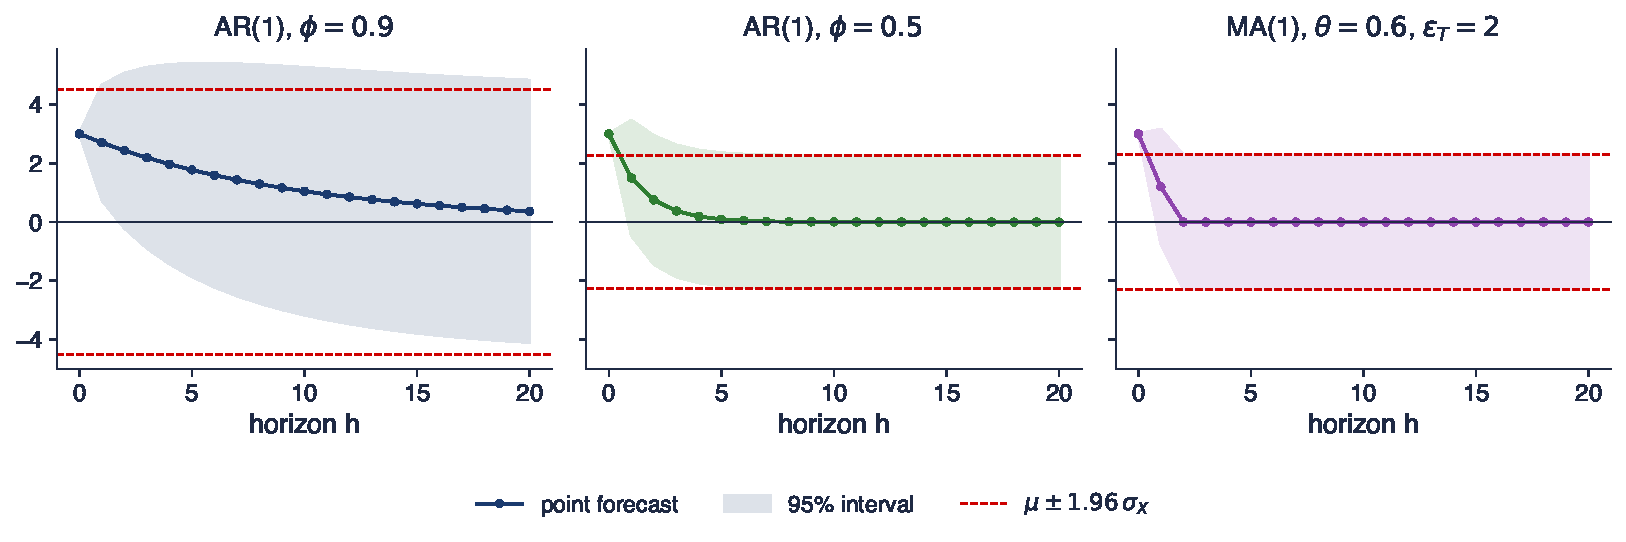
\includegraphics[width=0.97\textwidth,height=0.72\textheight,keepaspectratio]{tsa_ch2_forecast_theory.pdf}
\end{center}
\vspace{-0.25cm}
\begin{itemize}
    \item Pornire din $X_T = 3$, $\mu = 0$, $\sigma = 1$; linie întreruptă: banda necondiționată $\mu \pm 1{,}96\,\sigma_X$
\end{itemize}
\quantlet{TSA\_ch2\_forecasting}{\qlurl{TSA_ch2_forecasting}}
\end{frame}

\begin{frame}{Interpretarea traiectoriilor de prognoză}
\itemsize{\small}
\begin{itemize}
    \item $\phi = 0{,}9$: revenire lentă; după 5 perioade prognoza este încă 1{,}77, eroarea standard 1{,}85
    \begin{itemize}
        \item intervalul se apropie de $\pm 1{,}96 \times 2{,}29$ abia după multe perioade
    \end{itemize}
    \item $\phi = 0{,}5$: după 5 perioade prognoza este 0{,}094, practic media
    \item MA(1): un singur pas informativ ($\theta\varepsilon_T = 1{,}2$), apoi media; intervalul atinge lățimea de lungă durată la $h = 2$
    \item Un model staționar prognozează întotdeauna revenirea la medie: util pentru spread-uri și rate de creștere, înșelător dacă media se schimbă
\end{itemize}
\end{frame}

\begin{frame}{Recapitulare: prognoza}
\itemsize{\small}
\begin{itemize}
    \item $\hat X_{T+h|T}$: înlocuim șocurile viitoare cu 0 și valorile viitoare cu prognoze
    \item Varianța erorii $\sigma^2\sum_{j<h}\psi_j^2$; intervalele se lărgesc pînă la $\pm 1{,}96\sqrt{\gamma(0)}$
    \item Prognozele revin la $\mu$; prognozele MA($q$) sînt egale cu $\mu$ după $q$ pași
    \item Intervalele ignoră incertitudinea parametrilor și a modelului
\end{itemize}
\end{frame}


%=============================================================================
\section{Metoda Box--Jenkins}
%=============================================================================

\begin{frame}{George Box și Gwilym Jenkins}
\itemsize{\footnotesize}
\begin{columns}[T]
\begin{column}{0.62\textwidth}
\begin{itemize}
    \item \textbf{George E. P. Box} (1919--2013), statistician, Universitatea Wisconsin--Madison
    \begin{itemize}
        \item „Toate modelele sînt greșite, dar unele sînt utile”
    \end{itemize}
    \item \textbf{Gwilym M. Jenkins} (1932--1982), statistician, Universitatea Lancaster
    \begin{itemize}
        \item \textit{Time Series Analysis: Forecasting and Control}, 1970; a patra ediție, cu Reinsel: \refBJ
    \end{itemize}
    \item Contribuția lor: nu modele noi, ci o \textbf{metodă}
    \begin{itemize}
        \item o buclă de identificare, estimare și verificare pe care o poate aplica oricine
        \item testele Box--Pierce (1970) și Ljung--Box (1978) provin din acest program
    \end{itemize}
\end{itemize}
\end{column}
\begin{column}{0.34\textwidth}
\centering
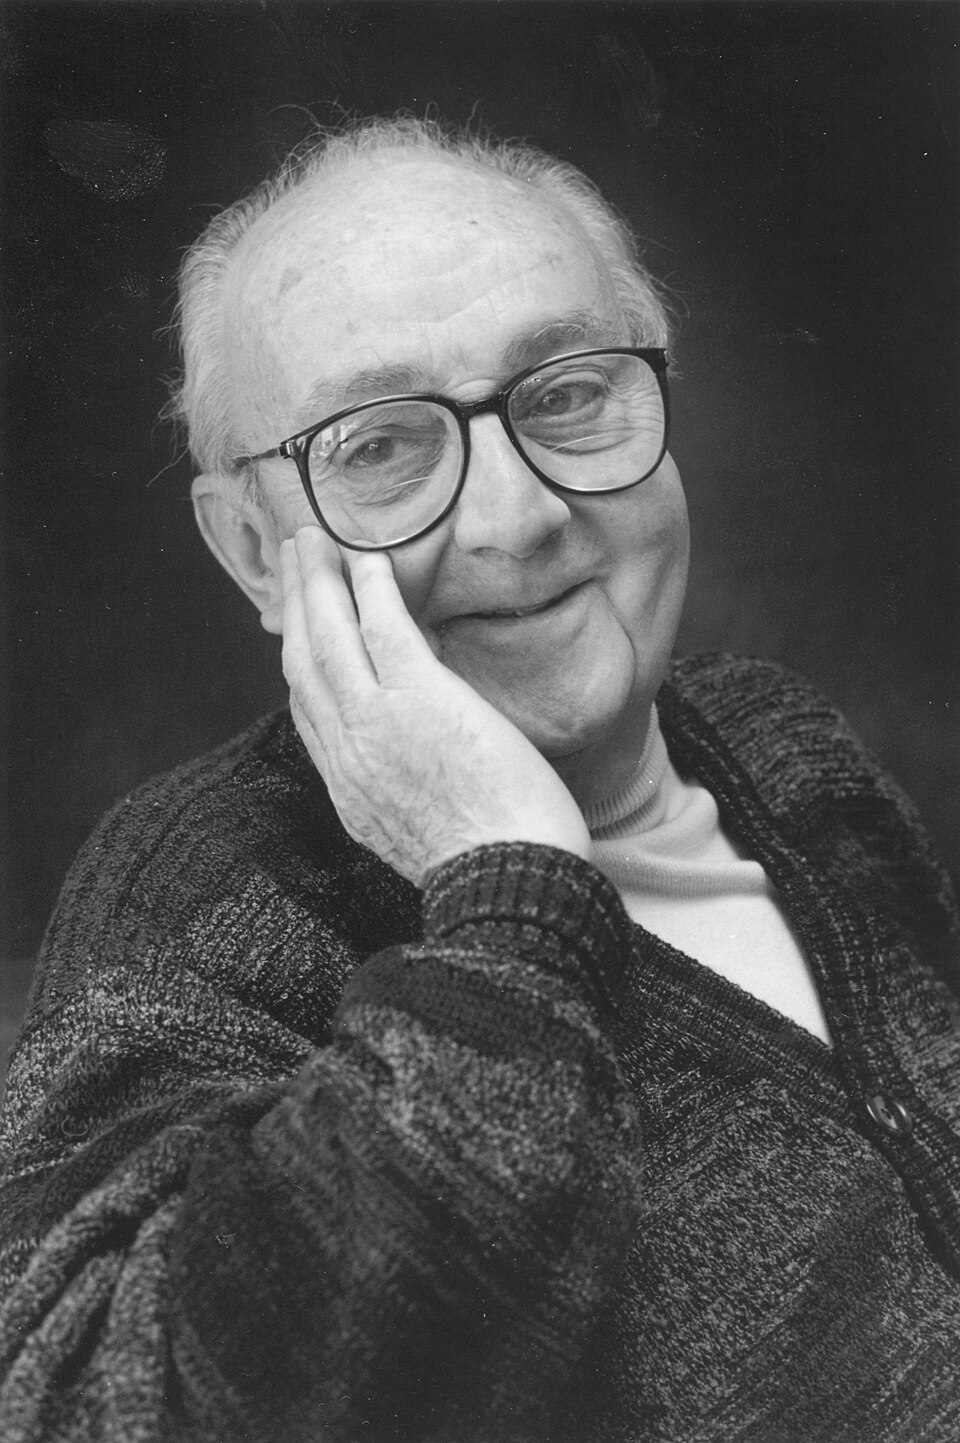
\includegraphics[height=0.50\textheight]{ch2_george_box.jpg}\\[1mm]
\imgcap{George E. P. Box}
\imgcredit{https://commons.wikimedia.org/wiki/File:GeorgeEPBox.jpg}{Foto: DavidMCEddy; CC BY-SA 3.0; Wikimedia Commons}
\end{column}
\end{columns}
\end{frame}

\begin{frame}{Bucla Box--Jenkins}
\itemsize{\footnotesize}
\begin{center}
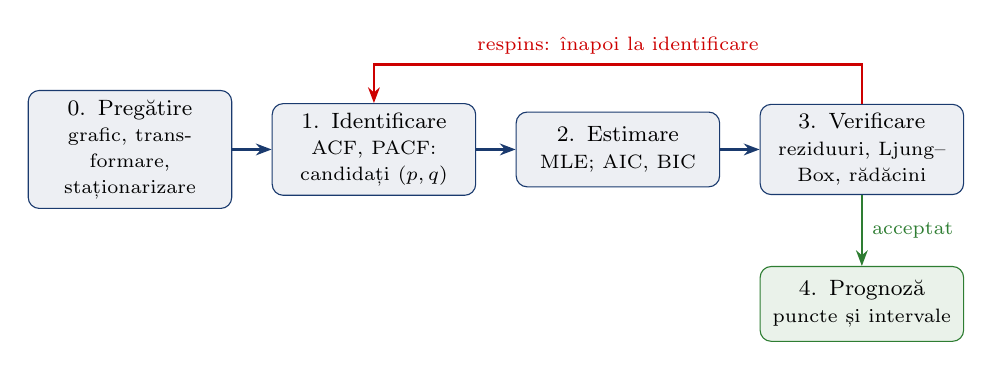
\begin{tikzpicture}[node distance=0.55cm and 0.5cm, font=\footnotesize,
  bx/.style={draw=MainBlue, rounded corners, fill=MainBlue!8, align=center, minimum height=0.95cm, text width=2.35cm},
  ar/.style={-{Stealth[length=2mm]}, thick, MainBlue}]
\node[bx] (a) {0. Pregătire\\{\scriptsize grafic, transformare, staționarizare}};
\node[bx, right=of a] (b) {1. Identificare\\{\scriptsize ACF, PACF: candidați $(p,q)$}};
\node[bx, right=of b] (c) {2. Estimare\\{\scriptsize MLE; AIC, BIC}};
\node[bx, right=of c] (d) {3. Verificare\\{\scriptsize reziduuri, Ljung--Box, rădăcini}};
\node[bx, below=0.9cm of d, fill=Forest!10, draw=Forest] (e) {4. Prognoză\\{\scriptsize puncte și intervale}};
\draw[ar] (a) -- (b); \draw[ar] (b) -- (c); \draw[ar] (c) -- (d);
\draw[ar, Forest] (d) -- node[right, font=\scriptsize, text=Forest] {acceptat} (e);
\draw[ar, IDAred] (d.north) -- ++(0, 0.5) -| node[pos=0.25, above, font=\scriptsize, text=IDAred] {respins: înapoi la identificare} (b.north);
\end{tikzpicture}
\end{center}
\begin{itemize}
    \item Pasul 0 ține de \tsachlink{https://danpele.github.io/Time-Series-Analysis/RO/Cursuri/capitol1_procese_stochastice_stationaritate.pdf}{Capitolele 1} și \tsachlink{https://danpele.github.io/Time-Series-Analysis/RO/Cursuri/capitol3_radacini_unitare_modele_arima.pdf}{3}: logaritmi, diferențe, teste de rădăcină unitară; ARMA cere o serie staționară
    \item Bucla se încheie cu cel mai mic model ale cărui reziduuri sînt zgomot alb și ale cărui rădăcini sînt bine în interiorul regiunii admise
    \item Verificările în afara eșantionului (\tsachlink{https://danpele.github.io/Time-Series-Analysis/RO/Cursuri/capitol0_introducere.pdf}{Capitolul 0}: eșantioane de antrenare și de test) completează metoda
\end{itemize}
\end{frame}

\begin{frame}{Recapitulare: metoda Box--Jenkins}
\itemsize{\small}
\begin{itemize}
    \item Pregătire, identificare, estimare, verificare, prognoză; revenim dacă verificarea eșuează
    \item Parcimonie: cel mai mic model adecvat
    \item Urmează: metoda aplicată PIB-ului României
\end{itemize}
\end{frame}


%=============================================================================
\section{Studiu de caz: creșterea PIB-ului României}
%=============================================================================

\begin{frame}{Datele}
\itemsize{\footnotesize}
\begin{columns}[T]
\begin{column}{0.60\textwidth}
\begin{itemize}
    \item PIB-ul real al României, volume înlănțuite (prețurile din 2010), trimestrial, neajustat sezonier; Eurostat, \texttt{namq\_10\_gdp}
    \begin{itemize}
        \item sursa națională: Institutul Național de Statistică (INS)
    \end{itemize}
    \item Creșterea anuală $y_t = 100\,(\ln Y_t - \ln Y_{t-4})$, în \%: elimină sezonalitatea (\tsachlink{https://danpele.github.io/Time-Series-Analysis/RO/Cursuri/capitol1_procese_stochastice_stationaritate.pdf}{Capitolul 1})
    \begin{itemize}
        \item T1 2000--T2 2026: $T = 106$ trimestre, media 3{,}29\%, abaterea standard 4{,}35\%
        \item extremele: $-9{,}9\%$ în T2 2020, $+12{,}5\%$ în T4 2004; ultima valoare $-2{,}0\%$
    \end{itemize}
    \item Este staționară? Rata de creștere nu are trend; testul formal este în \tsachlink{https://danpele.github.io/Time-Series-Analysis/RO/Cursuri/capitol3_radacini_unitare_modele_arima.pdf}{Capitolul 3}
\end{itemize}
\end{column}
\begin{column}{0.36\textwidth}
\centering
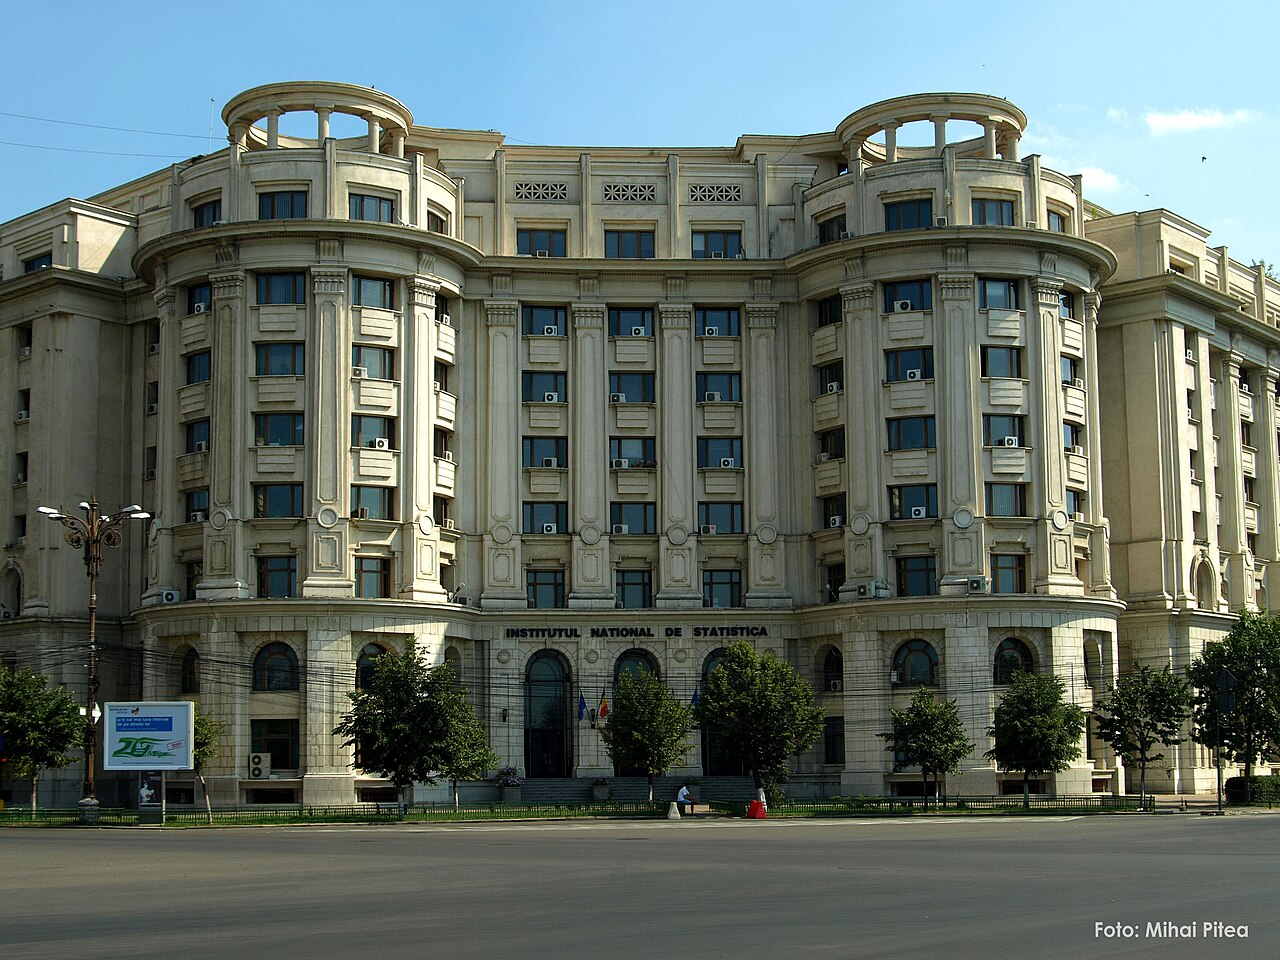
\includegraphics[height=0.42\textheight]{ch2_ins_bucharest_2009.jpg}\\[1mm]
\imgcap{Institutul Național de Statistică, București}
\imgcredit{https://commons.wikimedia.org/wiki/File:Institutul_Na\%C8\%9Bional_de_Statistic\%C4\%83.jpg}{Foto: Dan Mihai Pitea (2009); CC BY-SA 3.0; Wikimedia Commons}
\end{column}
\end{columns}
\end{frame}

\begin{frame}{Pasul 1: identificarea}
\itemsize{\footnotesize}
\begin{center}
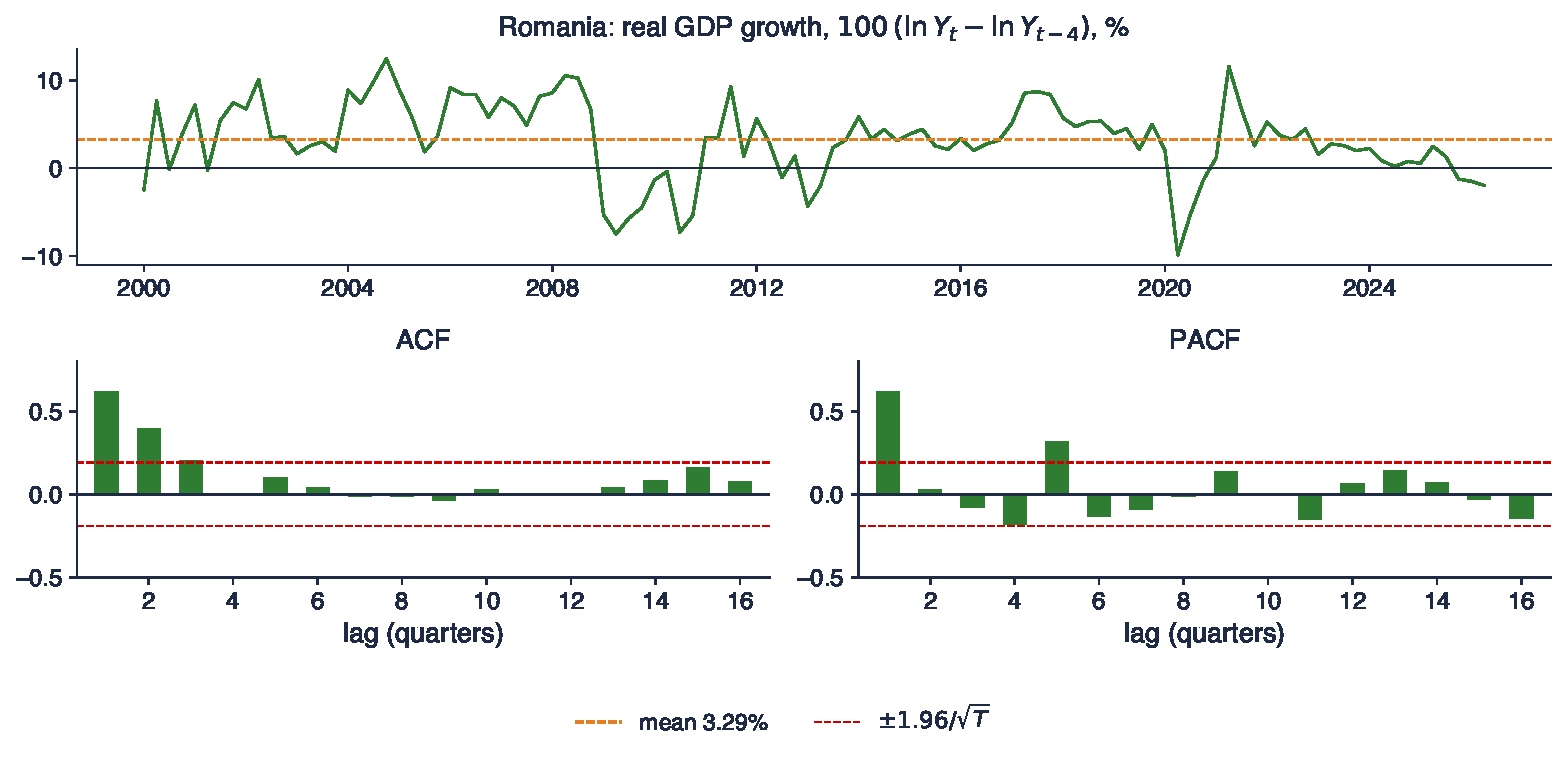
\includegraphics[width=0.97\textwidth,height=0.72\textheight,keepaspectratio]{tsa_ch2_gdp_ident.pdf}
\end{center}
\vspace{-0.25cm}
\begin{itemize}
    \item Creșterea anuală a PIB-ului real al României, ACF și PACF cu $\pm 1{,}96/\sqrt{T} = \pm 0{,}19$
\end{itemize}
\quantlet{TSA\_ch2\_gdp\_case}{\qlurl{TSA_ch2_gdp_case}}
\end{frame}

\begin{frame}{Interpretarea corelogramelor creșterii PIB}
\itemsize{\small}
\begin{itemize}
    \item ACF: $0{,}62$; $0{,}40$; $0{,}21$, apoi $-0{,}01$ la decalajul 4: \textbf{se anulează după decalajul 3}
    \begin{itemize}
        \item candidat: MA(3)
    \end{itemize}
    \item PACF: $0{,}62$ la decalajul 1, apoi valori mici, cu excepția lui $0{,}32$ la decalajul 5
    \begin{itemize}
        \item candidat: AR(1); decalajul 5 poate fi întîmplător sau o urmă a sezonalității
    \end{itemize}
    \item De ce MA(3)? $y_t$ este suma a patru rate trimestriale de creștere, $y_t \approx g_t + g_{t-1} + g_{t-2} + g_{t-3}$
    \begin{itemize}
        \item dacă $g_t$ este aproape de un zgomot alb (Seminarul 2, B2), ratele anuale consecutive au trei trimestre comune: un MA(3) prin construcție
    \end{itemize}
    \item Ljung--Box $Q^*(8) = 64{,}9$ pentru seria însăși: puternic autocorelată, deci este nevoie de un model
\end{itemize}
\end{frame}

\begin{frame}{Pasul 2: estimarea și criteriile informaționale}
\itemsize{\footnotesize}
\begin{center}
\footnotesize
\begin{tabular}{lrrrrrr}
\toprule
\textbf{Modelul} & $k$ & $\ln L$ & \textbf{AIC} & \textbf{BIC} & $\hat\sigma$ & \textbf{LB, valoarea p} \\
\midrule
ARMA(0,0) & 2 & $-305{,}83$ & 615{,}66 & 620{,}99 & 4{,}33 & $<$\,0{,}001 \\
ARMA(1,0) & 3 & $-279{,}67$ & 565{,}33 & 573{,}32 & 3{,}38 & 0{,}023 \\
ARMA(2,0) & 4 & $-279{,}66$ & 567{,}32 & 577{,}98 & 3{,}38 & 0{,}037 \\
ARMA(1,1) & 4 & $-279{,}66$ & 567{,}32 & 577{,}98 & 3{,}38 & 0{,}013 \\
ARMA(0,3) & 5 & $-270{,}02$ & 550{,}04 & 563{,}36 & 3{,}07 & 0{,}375 \\
ARMA(1,3) & 6 & $-268{,}48$ & 548{,}97 & 564{,}95 & 3{,}02 & 0{,}648 \\
ARMA(2,3) & 7 & $-267{,}94$ & 549{,}89 & 568{,}53 & 3{,}00 & 0{,}543 \\
\bottomrule
\end{tabular}
\end{center}
\begin{itemize}
    \item MLE exactă gaussiană pe aceleași 106 trimestre; LB = Ljung--Box $Q^*(8)$ pentru reziduuri, cu $8 - p - q$ grade de libertate; grila completă $p, q \le 3$ în Quantlet
    \item \textbf{BIC} alege MA(3); \textbf{AIC} alege ARMA(1,3), mai mic cu doar 1{,}07
    \item AR(1), candidatul sugerat de PACF, lasă autocorelație: valoarea p a testului LB este 0{,}023
\end{itemize}
\end{frame}

\begin{frame}{Interpretarea modelului MA(3) estimat}
\itemsize{\small}
\begin{itemize}
    \item $\hat y_t = 3{,}17 + \hat\varepsilon_t + 0{,}834\,\hat\varepsilon_{t-1} + 0{,}675\,\hat\varepsilon_{t-2} + 0{,}591\,\hat\varepsilon_{t-3}$, $\hat\sigma = 3{,}07$
    \begin{itemize}
        \item erorile standard: 1{,}03 (media), 0{,}083; 0{,}102; 0{,}082: toți cei trei termeni MA sînt semnificativi
    \end{itemize}
    \item Coeficienții $\hat\theta_j$ scad de la 0{,}834 la 0{,}591: aproape de tiparul suprapunerii $(1, 1, 1)$, dar sub el
    \begin{itemize}
        \item $(1, 1, 1)$ ar pune rădăcini pe cercul unitate; cel mai mic modul al rădăcinilor este aici 1{,}17 $> 1$: invertibil
    \end{itemize}
    \item ARMA(1,3): $\hat\theta_1 = 1{,}019 > 1$, dar rădăcinile au modulul cel puțin 1{,}10: tot invertibil
    \begin{itemize}
        \item pentru $q > 1$, invertibilitatea se citește din rădăcini, nu din coeficienți luați separat
        \item $\hat\phi = -0{,}284$ (eroarea standard 0{,}143): un parametru în plus pentru un cîștig mic; BIC renunță la el
    \end{itemize}
    \item Creșterea medie este de 3{,}17\% pe an, dar cu o eroare standard de 1{,}03: datele care se suprapun conțin mai puțină informație decît sugerează $T$
\end{itemize}
\end{frame}

\begin{frame}{Pasul 3: diagnosticarea modelului MA(3)}
\itemsize{\footnotesize}
\begin{center}
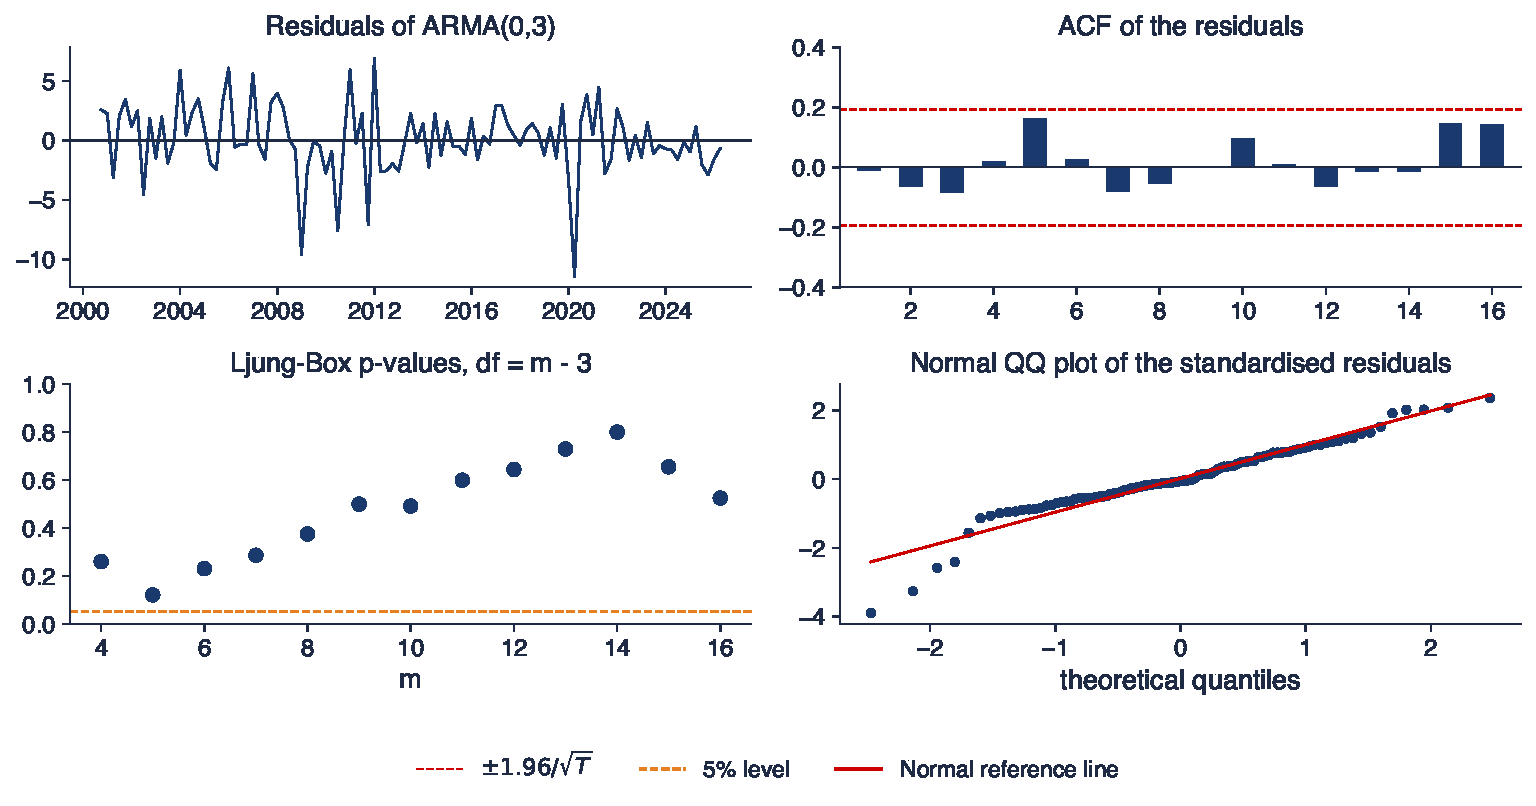
\includegraphics[width=0.97\textwidth,height=0.72\textheight,keepaspectratio]{tsa_ch2_gdp_diag.pdf}
\end{center}
\vspace{-0.25cm}
\begin{itemize}
    \item Reziduurile, ACF lor, valorile p ale testului Ljung--Box pentru $m = 4, \dots, 16$, cu $m - 3$ grade de libertate, graficul QQ față de distribuția Normală
\end{itemize}
\quantlet{TSA\_ch2\_gdp\_case}{\qlurl{TSA_ch2_gdp_case}}
\end{frame}

\begin{frame}{Interpretarea diagnosticării MA(3)}
\itemsize{\small}
\begin{itemize}
    \item Fără autocorelație în reziduuri: $Q^*(8) = 5{,}35$ cu 5 grade de libertate, p = 0{,}375; $Q^*(16)$: p = 0{,}525
    \begin{itemize}
        \item toate valorile p din grafic sînt peste 0{,}12; cu 8 în loc de 5 grade de libertate, p ar fi 0{,}720, prea liniștitor
    \end{itemize}
    \item Nu este Normal: Jarque--Bera 39{,}0, p $<$\,0{,}001; asimetria -0{,}75, boltirea 5{,}61
    \begin{itemize}
        \item cel mai mare reziduu: $-11{,}4$ în T2 2020, -3{,}89 abateri standard: perioada de lockdown din pandemie
    \end{itemize}
    \item Pătratele reziduurilor: testul Ljung--Box dă p = 0{,}779, fără volatility clustering la această frecvență
    \item Verdictul: MA(3) surprinde dependența; intervalele construite cu distribuția Normală subestimează riscul recesiunilor
\end{itemize}
\end{frame}

\begin{frame}{Pasul 4: prognozele}
\itemsize{\footnotesize}
\begin{center}
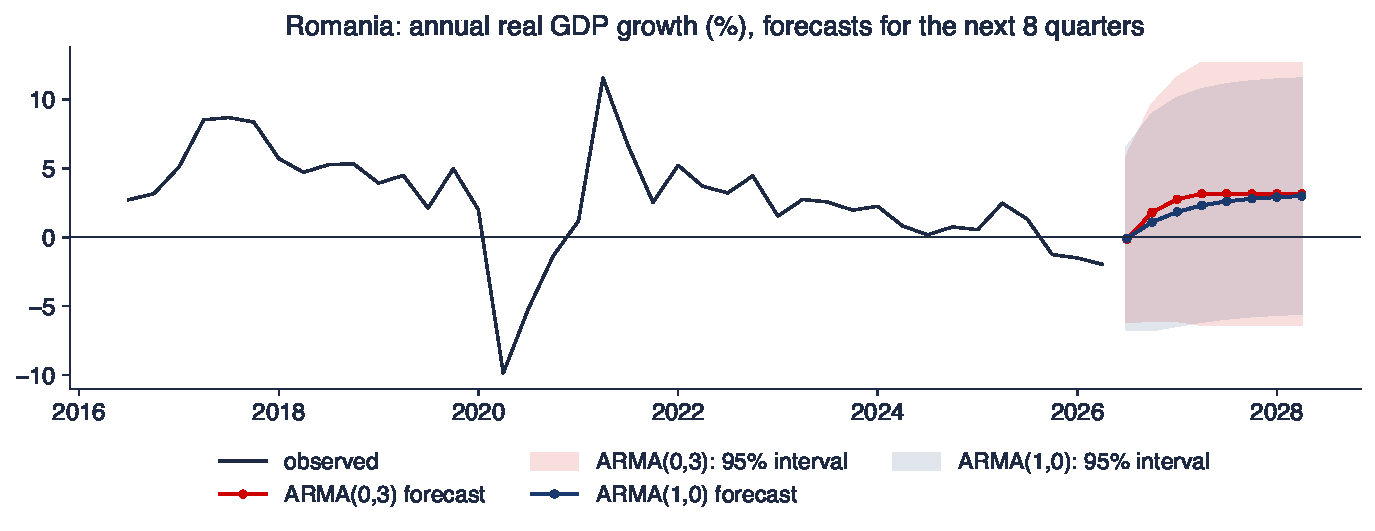
\includegraphics[width=0.97\textwidth,height=0.72\textheight,keepaspectratio]{tsa_ch2_gdp_forecast.pdf}
\end{center}
\vspace{-0.25cm}
\begin{itemize}
    \item Prognozele MA(3) (BIC) și AR(1) pentru T3 2026--T2 2028, cu intervale de 95\%
\end{itemize}
\quantlet{TSA\_ch2\_gdp\_case}{\qlurl{TSA_ch2_gdp_case}}
\end{frame}

\begin{frame}{Interpretarea prognozelor PIB}
\itemsize{\small}
\begin{itemize}
    \item MA(3): $-0{,}14$; $1{,}81$; $2{,}77$, apoi media de $3{,}17\%$ începînd cu al patrulea trimestru
    \begin{itemize}
        \item exact regula MA($q$): după $q = 3$ pași modelul cunoaște doar media
    \end{itemize}
    \item AR(1): o revenire netedă la medie, 2{,}99\% după 8 trimestre (media 3{,}12\%)
    \begin{itemize}
        \item cele două modele coincid pe termen scurt și diferă prin viteza cu care uită încetinirea recentă
    \end{itemize}
    \item Intervalele: $[-6{,}1; 5{,}9]$ pentru un trimestru, $[-6{,}3; 12{,}7]$ începînd cu patru trimestre: $\pm 6{,}0$ și $\pm 9{,}5$ puncte procentuale
    \item Un model univariat nu poate anticipa un punct de inflexiune; ne spune cît de neobișnuită ar fi următoarea valoare
\end{itemize}
\end{frame}

\begin{frame}{Recapitulare: creșterea PIB-ului României}
\itemsize{\small}
\begin{itemize}
    \item Creșterea anuală a PIB-ului trimestrial: ACF se anulează după decalajul 3, MA(3) după BIC, ARMA(1,3) după AIC
    \item MA(3) reflectă suprapunerea a patru trimestre: structura datelor explică modelul
    \item Reziduuri de tip zgomot alb, dar cozi groase (2020): intervalele sînt prea înguste în crize
    \item Prognozele ajung la medie după trei trimestre
\end{itemize}
\end{frame}


%=============================================================================
\section{Alte serii reale}
%=============================================================================

\begin{frame}{Inflația în România: o prognoză AR(2)}
\itemsize{\footnotesize}
\begin{center}
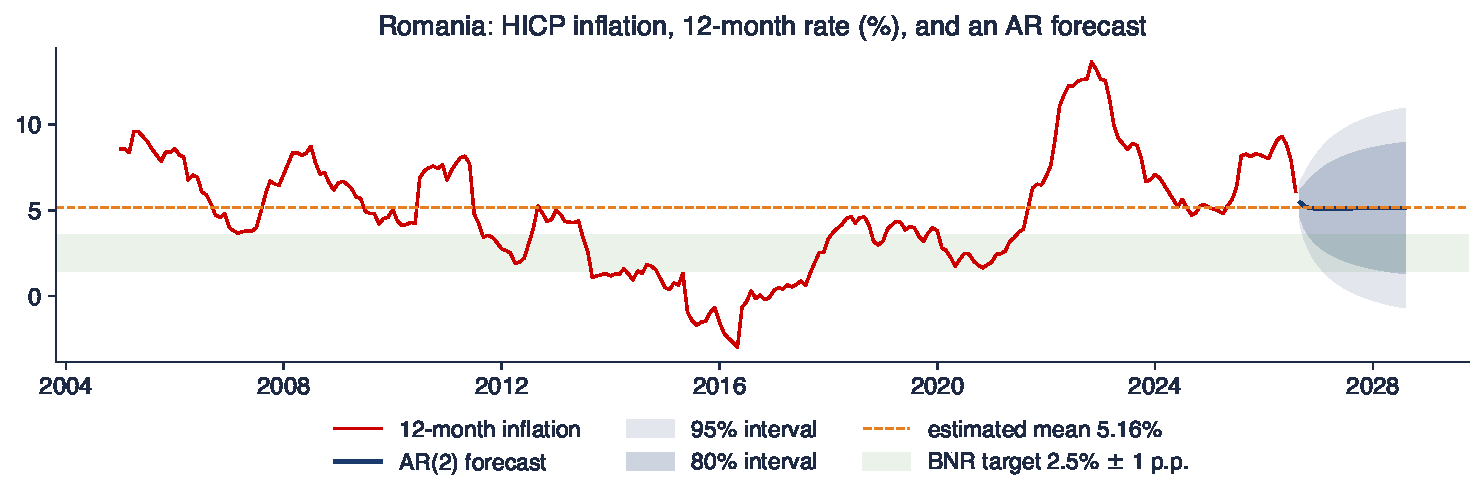
\includegraphics[width=0.97\textwidth,height=0.72\textheight,keepaspectratio]{tsa_ch2_inflation.pdf}
\end{center}
\vspace{-0.25cm}
\begin{itemize}
    \item IAPC (indicele armonizat al prețurilor de consum, Eurostat), rata pe 12 luni în \%, 260 de luni pînă în august 2026; ordinul AR ales prin BIC dintre $p \le 6$
\end{itemize}
\quantlet{TSA\_ch2\_real\_series}{\qlurl{TSA_ch2_real_series}}
\end{frame}

\begin{frame}{Interpretarea modelului pentru inflație}
\itemsize{\footnotesize}
\begin{itemize}
    \item BIC: 495{,}7 pentru AR(1), 469{,}7 pentru AR(2), 473{,}4 pentru AR(3): AR(2)
    \begin{itemize}
        \item $\hat\phi_1 = 1{,}320$ (0{,}057), $\hat\phi_2 = -0{,}344$ (0{,}055); $\hat\phi_1 + \hat\phi_2 = 0{,}976$, cea mai mare rădăcină inversă 0{,}963
    \end{itemize}
    \item Foarte aproape de o rădăcină unitară: este inflația staționară? Testul este în \tsachlink{https://danpele.github.io/Time-Series-Analysis/RO/Cursuri/capitol3_radacini_unitare_modele_arima.pdf}{Capitolul 3}
    \begin{itemize}
        \item media estimată, $5{,}16\%$ (eroarea standard 1{,}35), este media perioadei 2005--2026, peste ținta BNR de 2,5\% $\pm$ 1 p.p.
    \end{itemize}
    \item Prognoza: de la 6{,}09\% la 5{,}44\% luna viitoare și 5{,}13\% în august 2028; intervalul de 95\%: $[-0{,}6; 10{,}9]$
    \begin{itemize}
        \item modelul revine la media istorică, nu la țintă: nu știe nimic despre politica monetară
    \end{itemize}
    \item Diagnosticarea eșuează: Ljung--Box $Q^*(12) = 71{,}6$, p $<$\,0{,}001: corelație la decalajul 12 (efectele de bază ale ratei pe 12 luni), o temă pentru \tsachlink{https://danpele.github.io/Time-Series-Analysis/RO/Cursuri/capitol4_sezonalitate_prognoza.pdf}{Capitolul 4}
\end{itemize}
\end{frame}

\begin{frame}{Randamente zilnice: BET și EUR/RON}
\itemsize{\footnotesize}
\begin{center}
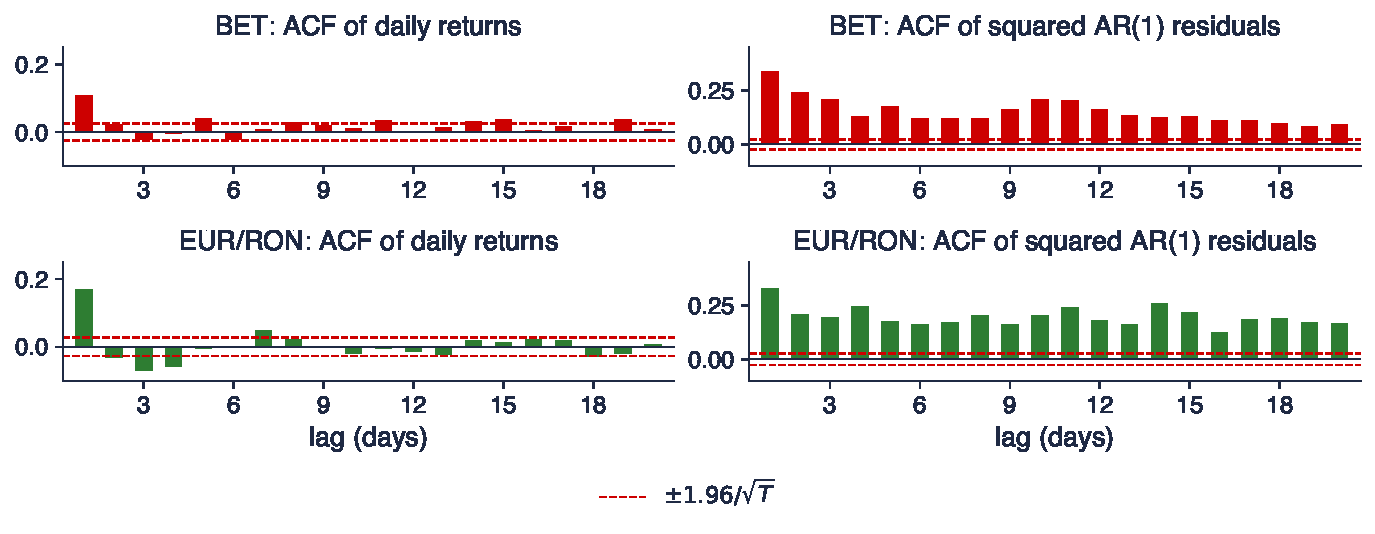
\includegraphics[width=0.97\textwidth,height=0.72\textheight,keepaspectratio]{tsa_ch2_returns.pdf}
\end{center}
\vspace{-0.25cm}
\begin{itemize}
    \item Stînga: ACF a randamentelor logaritmice zilnice; dreapta: ACF a pătratelor reziduurilor unui AR(1)
\end{itemize}
\quantlet{TSA\_ch2\_real\_series}{\qlurl{TSA_ch2_real_series}}
\end{frame}

\begin{frame}{Interpretarea modelului AR(1) pentru randamentele zilnice}
\itemsize{\footnotesize}
\begin{center}
\footnotesize
\begin{tabular}{lrr}
\toprule
 & \textbf{BET} & \textbf{EUR/RON} \\
\midrule
Observații & 6\,670 & 5\,352 \\
$\hat\phi$ (se) & $0{,}109$ (0{,}005) & $0{,}170$ (0{,}006) \\
Raportul $t$ & 20{,}9 & 30{,}6 \\
$R^2$ (\%) & 1{,}2 & 2{,}9 \\
LB $Q^*(10)$ reziduuri, 9 g.l. (p) & 29{,}7 ($<$\,0{,}001) & 61{,}5 ($<$\,0{,}001) \\
LB $Q^*(10)$ pătratele reziduurilor & 2496 & 2351 \\
Boltirea reziduurilor & 14{,}0 & 17{,}0 \\
Alegerea BIC, $p, q \le 2$ & ARMA(1,0) & ARMA(2,1) \\
\bottomrule
\end{tabular}
\end{center}
\begin{itemize}
    \item $\hat\phi$ foarte semnificativ, dar un $R^2$ de 1--3\%: real din punct de vedere \textbf{statistic}, mic din punct de vedere \textbf{economic} după costurile de tranzacționare
    \item $\hat\phi$ pozitiv: ajustarea lentă a prețurilor (BET), un curs de schimb administrat (EUR/RON)
    \item Pătratele reziduurilor și boltirea: media este modelată, varianța nu; ARMA + GARCH în \tsachlink{https://danpele.github.io/Time-Series-Analysis/RO/Cursuri/capitol5_volatilitate_conditionata_garch.pdf}{Capitolul 5}
\end{itemize}
\end{frame}

\begin{frame}{Studiu de caz: Yule (1927) și petele solare}
\itemsize{\footnotesize}
\begin{itemize}
    \item \refYule{} a estimat prima autoregresie: numerele anuale ale petelor solare ale lui Wolfer, 1749--1924
    \begin{itemize}
        \item pînă atunci, ciclurile erau modelate ca sume de sinusoide (periodograma)
        \item Yule: un „pendul bombardat cu mazăre”: un oscilator amortizat lovit de șocuri aleatoare
    \end{itemize}
    \item AR(2)-ul nostru, estimat prin cele mai mici pătrate pe aceiași ani (176 de observații, datele din statsmodels):
    \begin{itemize}
        \item $\hat\phi_1 = 1{,}336$, $\hat\phi_2 = -0{,}650$: rădăcini complexe, modulul rădăcinilor inverse 0{,}806
        \item perioada implicită $2\pi/\arccos(\hat\phi_1/(2\sqrt{-\hat\phi_2})) = 10{,}57$ ani: ciclul solar, din doar doi coeficienți
    \end{itemize}
    \item \refWalker{} a generalizat ecuațiile la AR($p$): ecuațiile Yule--Walker
    \begin{itemize}
        \item începutul analizei parametrice a seriilor de timp
    \end{itemize}
\end{itemize}
\end{frame}

\begin{frame}{Petele solare: AR(2) și criteriile informaționale}
\itemsize{\footnotesize}
\begin{center}
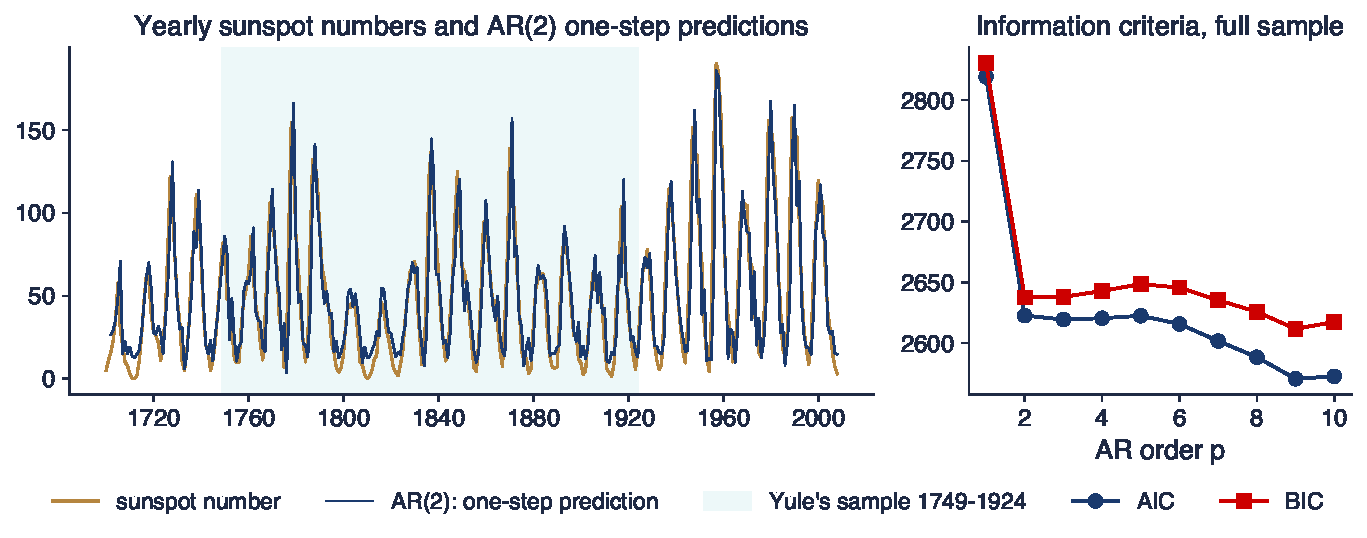
\includegraphics[width=0.97\textwidth,height=0.72\textheight,keepaspectratio]{tsa_ch2_sunspots.pdf}
\end{center}
\vspace{-0.25cm}
\begin{itemize}
    \item Numerele anuale ale petelor solare, 1700--2008 (309 ani); AR($p$) prin MLE pe întregul eșantion
\end{itemize}
\quantlet{TSA\_ch2\_real\_series}{\qlurl{TSA_ch2_real_series}}
\end{frame}

\begin{frame}{Interpretarea modelelor pentru petele solare}
\itemsize{\small}
\begin{itemize}
    \item AR(2) pe întregul eșantion: $\hat\phi = (1{,}391; -0{,}689)$, apropiat de cel al lui Yule; explică 83\% din varianță cu un an înainte
    \begin{itemize}
        \item predicțiile cu un pas urmează ciclul, dar întîrzie la vîrfuri
    \end{itemize}
    \item AIC și BIC aleg amîndouă $p = 9$ dintre $p \le 10$
    \begin{itemize}
        \item ciclul este asimetric (creștere rapidă, scădere lentă), ceea ce un AR(2) liniar nu poate reproduce
    \end{itemize}
    \item Lecția: doi parametri surprind esențialul; mai multe decalaje surprind detaliile; neliniaritatea depășește cadrul ARMA
\end{itemize}
\end{frame}

\begin{frame}{Studiu de caz: competițiile de prognoză}
\itemsize{\small}
\begin{itemize}
    \item \refMH: competiția M3, 3003 serii (anuale, trimestriale, lunare, altele), 24 de metode
    \begin{itemize}
        \item prognoze comparate în afara eșantionului, după mai multe măsuri de acuratețe și orizonturi
    \end{itemize}
    \item Concluzii confirmate față de competițiile M anterioare
    \begin{itemize}
        \item metodele sofisticate statistic nu prognozează neapărat mai bine decît cele simple
        \item clasamentul depinde de măsura de acuratețe și de orizont; combinațiile de metode se descurcă bine
    \end{itemize}
    \item Consecințe pentru ARMA
    \begin{itemize}
        \item bucla Box--Jenkins trebuie să se încheie cu o comparație în afara eșantionului cu repere simple (media, ultima valoare, netezirea exponențială din \tsachlink{https://danpele.github.io/Time-Series-Analysis/RO/Cursuri/capitol0_introducere.pdf}{Capitolul 0})
        \item Seminarul 2, C1 face această comparație pentru inflația din România
    \end{itemize}
\end{itemize}
\end{frame}

\begin{frame}{Recapitulare: alte serii reale}
\itemsize{\small}
\begin{itemize}
    \item Inflația: AR(2) aproape de o rădăcină unitară; revine la media istorică; corelație reziduală la decalajul 12
    \item Randamentele zilnice: efecte AR semnificative, dar foarte mici; varianța cere GARCH
    \item Petele solare: AR(2)-ul lui Yule dă ciclul de 11 ani din rădăcini complexe
    \item Competițiile de prognoză: comparați întotdeauna cu repere simple
\end{itemize}
\end{frame}


%=============================================================================
\section{Contribuția posibilă a AI}
%=============================================================================

\begin{frame}{Contribuția posibilă a AI}
\itemsize{\small}
\begin{itemize}
    \item \textbf{Cod}: o primă versiune a unei bucle care estimează ARMA($p,q$) pe o grilă, tabelează AIC și BIC și aplică testele pe reziduuri
    \item \textbf{Explicații}: o a doua deducere a ACF pentru un ARMA(1,1) sau a motivului pentru care PACF a unui MA descrește
    \item \textbf{Explorare}: aceeași buclă Box--Jenkins pe multe serii (creșterea PIB a tuturor țărilor UE), pentru a compara persistența
    \item Exemplu de prompt
    \begin{itemize}
        \item \aiprompt{Write Python code with statsmodels that fits ARMA(p,q), p,q <= 3, to Romanian annual GDP growth from Eurostat, reports AIC, BIC and the Ljung-Box p-value with model\_df = p + q, and forecasts 8 quarters from the BIC model.}
    \end{itemize}
\end{itemize}
\end{frame}

\begin{frame}{Verificări necesare}
\itemsize{\small}
\begin{itemize}
    \item Convenția de semn pentru $\theta$ și $\phi$ în program ($\theta(L) = 1 + \theta L$ în statsmodels, $1 - \theta L$ în unele manuale)
    \item Termenul liber sau media: \texttt{const} din \texttt{ARIMA} este media $\mu$, nu $c$
    \item Gradele de libertate ale testului Ljung--Box pentru reziduuri ($m - p - q$) și faptul că toate modelele sînt comparate pe același eșantion
    \item Rădăcinile ambelor polinoame, nu mărimea coeficienților luați separat
    \item Că seria este staționară înainte de estimarea unui ARMA (\tsachlink{https://danpele.github.io/Time-Series-Analysis/RO/Cursuri/capitol3_radacini_unitare_modele_arima.pdf}{Capitolul 3}) și că prognozele sînt comparate cu repere simple
    \item Fiecare referință citată: trebuie să existe; verificați DOI-ul
\end{itemize}
\end{frame}


%=============================================================================
\section{Rezumat}
%=============================================================================

\begin{frame}{Idei de reținut}
\itemsize{\small}
\begin{itemize}
    \item ARMA($p,q$) înlocuiește suma Wold infinită cu raportul a două polinoame scurte, $\theta(L)/\phi(L)$
    \item Staționaritatea: rădăcinile lui $\phi(z)$ în afara cercului unitate; invertibilitatea: rădăcinile lui $\theta(z)$ în afara lui; fără factori comuni
    \item ACF se anulează: MA; PACF se anulează: AR; ambele descresc: ARMA
    \item Estimați prin MLE, alegeți cu AIC/BIC, verificați reziduurile cu Ljung--Box pe $m - p - q$ grade de libertate
    \item Prognozele revin la medie; intervalele se lărgesc pînă la $\pm 1{,}96\sqrt{\gamma(0)}$ și ignoră incertitudinea parametrilor
    \item Datele reale: creșterea PIB este un MA(3) prin construcție; inflația este aproape de o rădăcină unitară; randamentele cer GARCH
\end{itemize}
\end{frame}

\begin{frame}{Formule de reținut}
\itemsize{\small}
{\renewcommand{\arraystretch}{1.35}\begin{center}
\scriptsize
\begin{tabular}{ll}
\toprule
\textbf{Mărimea} & \textbf{Formula} \\
\midrule
ARMA($p,q$) & $\phi(L)(X_t - \mu) = \theta(L)\varepsilon_t$, \quad $\psi(L) = \theta(L)/\phi(L)$ \\
AR(1) & $\mu = c/(1 - \phi)$, \quad $\gamma(0) = \sigma^2/(1 - \phi^2)$, \quad $\rho(h) = \phi^h$ \\
AR(2) & $\rho(1) = \phi_1/(1 - \phi_2)$, \quad $\rho(h) = \phi_1\rho(h - 1) + \phi_2\rho(h - 2)$ \\
MA(1) & $\rho(1) = \theta/(1 + \theta^2)$, \quad $\rho(h) = 0$, $h \ge 2$; invertibil $|\theta| < 1$ \\
ARMA(1,1) & $\psi_j = \phi^{j-1}(\phi + \theta)$, \quad $\rho(h) = \phi\rho(h - 1)$, $h \ge 2$ \\
Yule--Walker & $\hat\phi = \hat R^{-1}\hat\rho$, \quad $\hat\sigma^2 = \hat\gamma(0)(1 - \hat\phi^\top\hat\rho)$ \\
Criterii & $\mathrm{AIC} = -2\ln L + 2k$, \quad $\mathrm{BIC} = -2\ln L + k\ln T$ \\
Reziduuri & $Q^*(m) \sim \chi^2(m - p - q)$ \\
Prognoză & $\hat X_{T+h|T} \pm 1{,}96\,\sigma\sqrt{\textstyle\sum_{j=0}^{h-1}\psi_j^2}$ \\
\bottomrule
\end{tabular}
\end{center}
}
\end{frame}

\begin{frame}{Autoevaluare}
\itemsize{\small}
\begin{itemize}
    \item \textbf{Întrebare}: este $X_t = 1{,}2X_{t-1} - 0{,}32X_{t-2} + \varepsilon_t$ staționar?
    \begin{itemize}
        \item \textbf{Răspuns}: $1 - 1{,}2z + 0{,}32z^2 = (1 - 0{,}8z)(1 - 0{,}4z)$, rădăcinile 1,25 și 2,5, ambele în afara cercului: da
    \end{itemize}
    \item \textbf{Întrebare}: ACF a unei serii are o singură valoare semnificativă, $\hat\rho(1) = -0{,}45$, iar PACF descrește. Ce model?
    \begin{itemize}
        \item \textbf{Răspuns}: MA(1) cu $\theta < 0$; rezolvăm $\theta/(1 + \theta^2) = -0{,}45$ și păstrăm rădăcina invertibilă
    \end{itemize}
    \item \textbf{Întrebare}: un ARMA(2,1) lasă în reziduuri $Q^*(10) = 15{,}2$. Respingem la 5\%?
    \begin{itemize}
        \item \textbf{Răspuns}: gradele de libertate $10 - 3 = 7$, $\chi^2_{0{,}95}(7) = 14{,}07 < 15{,}2$: respingem; cu 10 grade de libertate (valoarea critică 18,31) am accepta greșit
    \end{itemize}
    \item Urmează: \tsachlink{https://danpele.github.io/Time-Series-Analysis/RO/Cursuri/capitol3_radacini_unitare_modele_arima.pdf}{Capitolul 3}, rădăcini unitare și modele ARIMA: ce facem cînd o rădăcină se află pe cercul unitate
\end{itemize}
\end{frame}


%=============================================================================
\section{Bibliografie}
%=============================================================================

\begin{frame}{Bibliografie (1/2)}
\itemsize{\tiny}
\begin{itemize}
    \item Akaike, H. (1974). A new look at the statistical model identification. \textit{IEEE Transactions on Automatic Control}, 19(6), 716--723. \href{https://doi.org/10.1109/TAC.1974.1100705}{doi:10.1109/TAC.1974.1100705}
    \item Box, G. E. P., Jenkins, G. M., \& Reinsel, G. C. (2008). \textit{Time Series Analysis: Forecasting and Control} (4th ed.). Wiley. \href{https://doi.org/10.1002/9781118619193}{doi:10.1002/9781118619193}
    \item Box, G. E. P., \& Pierce, D. A. (1970). Distribution of residual autocorrelations in autoregressive-integrated moving average time series models. \textit{Journal of the American Statistical Association}, 65(332), 1509--1526. \href{https://doi.org/10.1080/01621459.1970.10481180}{doi:10.1080/01621459.1970.10481180}
    \item Brockwell, P. J., \& Davis, R. A. (1991). \textit{Time Series: Theory and Methods} (2nd ed.). Springer. \href{https://doi.org/10.1007/978-1-4419-0320-4}{doi:10.1007/978-1-4419-0320-4}
    \item Brockwell, P. J., \& Davis, R. A. (2016). \textit{Introduction to Time Series and Forecasting} (3rd ed.). Springer. \href{https://doi.org/10.1007/978-3-319-29854-2}{doi:10.1007/978-3-319-29854-2}
    \item Durbin, J. (1960). The fitting of time-series models. \textit{Revue de l\'Institut International de Statistique}, 28(3), 233--244. \href{https://doi.org/10.2307/1401322}{doi:10.2307/1401322}
    \item Hamilton, J. D. (1994). \textit{Time Series Analysis}. Princeton University Press. \href{https://doi.org/10.2307/j.ctv14jx6sm}{doi:10.2307/j.ctv14jx6sm}
    \item Huang, C., \& Petukhina, A. (2022). \textit{Applied Time Series Analysis and Forecasting with Python}. Springer. \href{https://doi.org/10.1007/978-3-031-13584-2}{doi:10.1007/978-3-031-13584-2}
    \item Hurvich, C. M., \& Tsai, C.-L. (1989). Regression and time series model selection in small samples. \textit{Biometrika}, 76(2), 297--307. \href{https://doi.org/10.1093/biomet/76.2.297}{doi:10.1093/biomet/76.2.297}
    \item Hyndman, R. J., \& Athanasopoulos, G. (2021). \textit{Forecasting: Principles and Practice} (3rd ed.). OTexts. \href{https://otexts.com/fpp3/}{otexts.com/fpp3}
    \item Hyndman, R. J., \& Khandakar, Y. (2008). Automatic time series forecasting: The forecast package for R. \textit{Journal of Statistical Software}, 27(3), 1--22. \href{https://doi.org/10.18637/jss.v027.i03}{doi:10.18637/jss.v027.i03}
    \item Jarque, C. M., \& Bera, A. K. (1987). A test for normality of observations and regression residuals. \textit{International Statistical Review}, 55(2), 163--172. \href{https://doi.org/10.2307/1403192}{doi:10.2307/1403192}
    \item Ljung, G. M., \& Box, G. E. P. (1978). On a measure of lack of fit in time series models. \textit{Biometrika}, 65(2), 297--303. \href{https://doi.org/10.1093/biomet/65.2.297}{doi:10.1093/biomet/65.2.297}
    \item Makridakis, S., \& Hibon, M. (2000). The M3-Competition: Results, conclusions and implications. \textit{International Journal of Forecasting}, 16(4), 451--476. \href{https://doi.org/10.1016/S0169-2070(00)00057-1}{doi:10.1016/S0169-2070(00)00057-1}
    \item Schwarz, G. (1978). Estimating the dimension of a model. \textit{The Annals of Statistics}, 6(2), 461--464. \href{https://doi.org/10.1214/aos/1176344136}{doi:10.1214/aos/1176344136}
    \item Slutzky, E. (1937). The summation of random causes as the source of cyclic processes. \textit{Econometrica}, 5(2), 105--146. \href{https://doi.org/10.2307/1907241}{doi:10.2307/1907241}
\end{itemize}
\end{frame}

\begin{frame}{Bibliografie (2/2)}
\itemsize{\tiny}
\begin{itemize}
    \item Walker, G. (1931). On periodicity in series of related terms. \textit{Proceedings of the Royal Society of London, Series A}, 131(818), 518--532. \href{https://doi.org/10.1098/rspa.1931.0069}{doi:10.1098/rspa.1931.0069}
    \item Wold, H. (1938). \textit{A Study in the Analysis of Stationary Time Series}. Almqvist \& Wiksell. \href{https://archive.org/details/in.ernet.dli.2015.262214}{archive.org}
    \item Yule, G. U. (1927). On a method of investigating periodicities in disturbed series, with special reference to Wolfer's sunspot numbers. \textit{Philosophical Transactions of the Royal Society A}, 226, 267--298. \href{https://doi.org/10.1098/rsta.1927.0007}{doi:10.1098/rsta.1927.0007}
\end{itemize}
\end{frame}

\end{document}
